% Created 2016-04-06 Wed 15:41
\documentclass[9pt]{beamer}
\usepackage[utf8]{inputenc}
\usepackage[T1]{fontenc}
\usepackage{fixltx2e}
\usepackage{graphicx}
\usepackage{longtable}
\usepackage{float}
\usepackage{wrapfig}
\usepackage{soul}
\usepackage{textcomp}
\usepackage{marvosym}
\usepackage{wasysym}
\usepackage{latexsym}
\usepackage{amssymb}
\usepackage{hyperref}
\tolerance=1000
\mode<beamer>{\usetheme{Warsaw}}
\mode<beamer>{\setbeamertemplate{blocks}[rounded][shadow=false]}
\mode<beamer>{\addtobeamertemplate{block begin}{\pgfsetfillopacity{0.8}}{\pgfsetfillopacity{1}}}
\mode<beamer>{\setbeamercolor{structure}{fg=orange}}
\mode<beamer>{\setbeamercovered{transparent}}
\AtBeginSection[]{\begin{frame}<beamer>\frametitle{Topic}\tableofcontents[currentsection]\end{frame}}
\usepackage{subcaption}
\usepackage{multimedia}
\usepackage{tikz}
\usepackage{subfigure,subfigmat}
\usepackage{threeparttable}
\usetikzlibrary{shapes,arrows,shadows}
\usepackage{bm, amssymb, amsmath, array, pdfpages}
\newcommand{\bv}[1]{\mathbf{#1}}
\newcommand{\diff}[2]{\frac{\partial #1}{\partial #2}}
\newcommand{\beq}[0]{\begin{equation}}
\newcommand{\eeq}[0]{\end{equation}}
\newcommand{\beqa}[0]{\begin{eqnarray}}
\newcommand{\eeqa}[0]{\end{eqnarray}}
\newcommand{\beqq}[0]{\begin{equation*}}
\newcommand{\eeqq}[0]{\end{equation*}}
\newcommand{\bs}[1]{\boldsymbol{#1}}
\newcommand{\ip}[2]{\langle #1, #2\rangle}
\providecommand{\alert}[1]{\textbf{#1}}

\title{Modeling and Uncertainty Quantification for Airfoil Icing}
\author{Anthony DeGennaro \newline Clarence W. Rowley III \newline Luigi Martinelli \newline Princeton University}
\date{Group Presentation \\ Princeton, NJ \\ March 2016}
\hypersetup{
  pdfkeywords={},
  pdfsubject={},
  pdfcreator={Emacs Org-mode version 7.9.3f}}

\begin{document}

\maketitle

\begin{frame}
\frametitle{Outline}
\setcounter{tocdepth}{3}
\tableofcontents
\end{frame}



% Define my settings

\graphicspath{{Figures/}}
% Add Princeton shield logo
\addtobeamertemplate{frametitle}{}{%
\begin{tikzpicture}[remember picture,overlay]
\node[anchor=north east,yshift=2pt] at (current page.north east) {
\includegraphics[height=0.7cm]{Shield}};
\end{tikzpicture}}
%


\institute{Princeton University}

\section{Motivation/Background}
\label{sec-1}
\begin{frame}
\frametitle{Introduction}
\label{sec-1-1}

\textbf{Wing icing deteriorates airfoil aerodynamics}
\begin{itemize}
\item Leading edge flow separation bubble
\item Lower lift, higher drag
\item Unpredictable stall
\end{itemize}

\vspace*{-0.0cm}\begin{figure}
    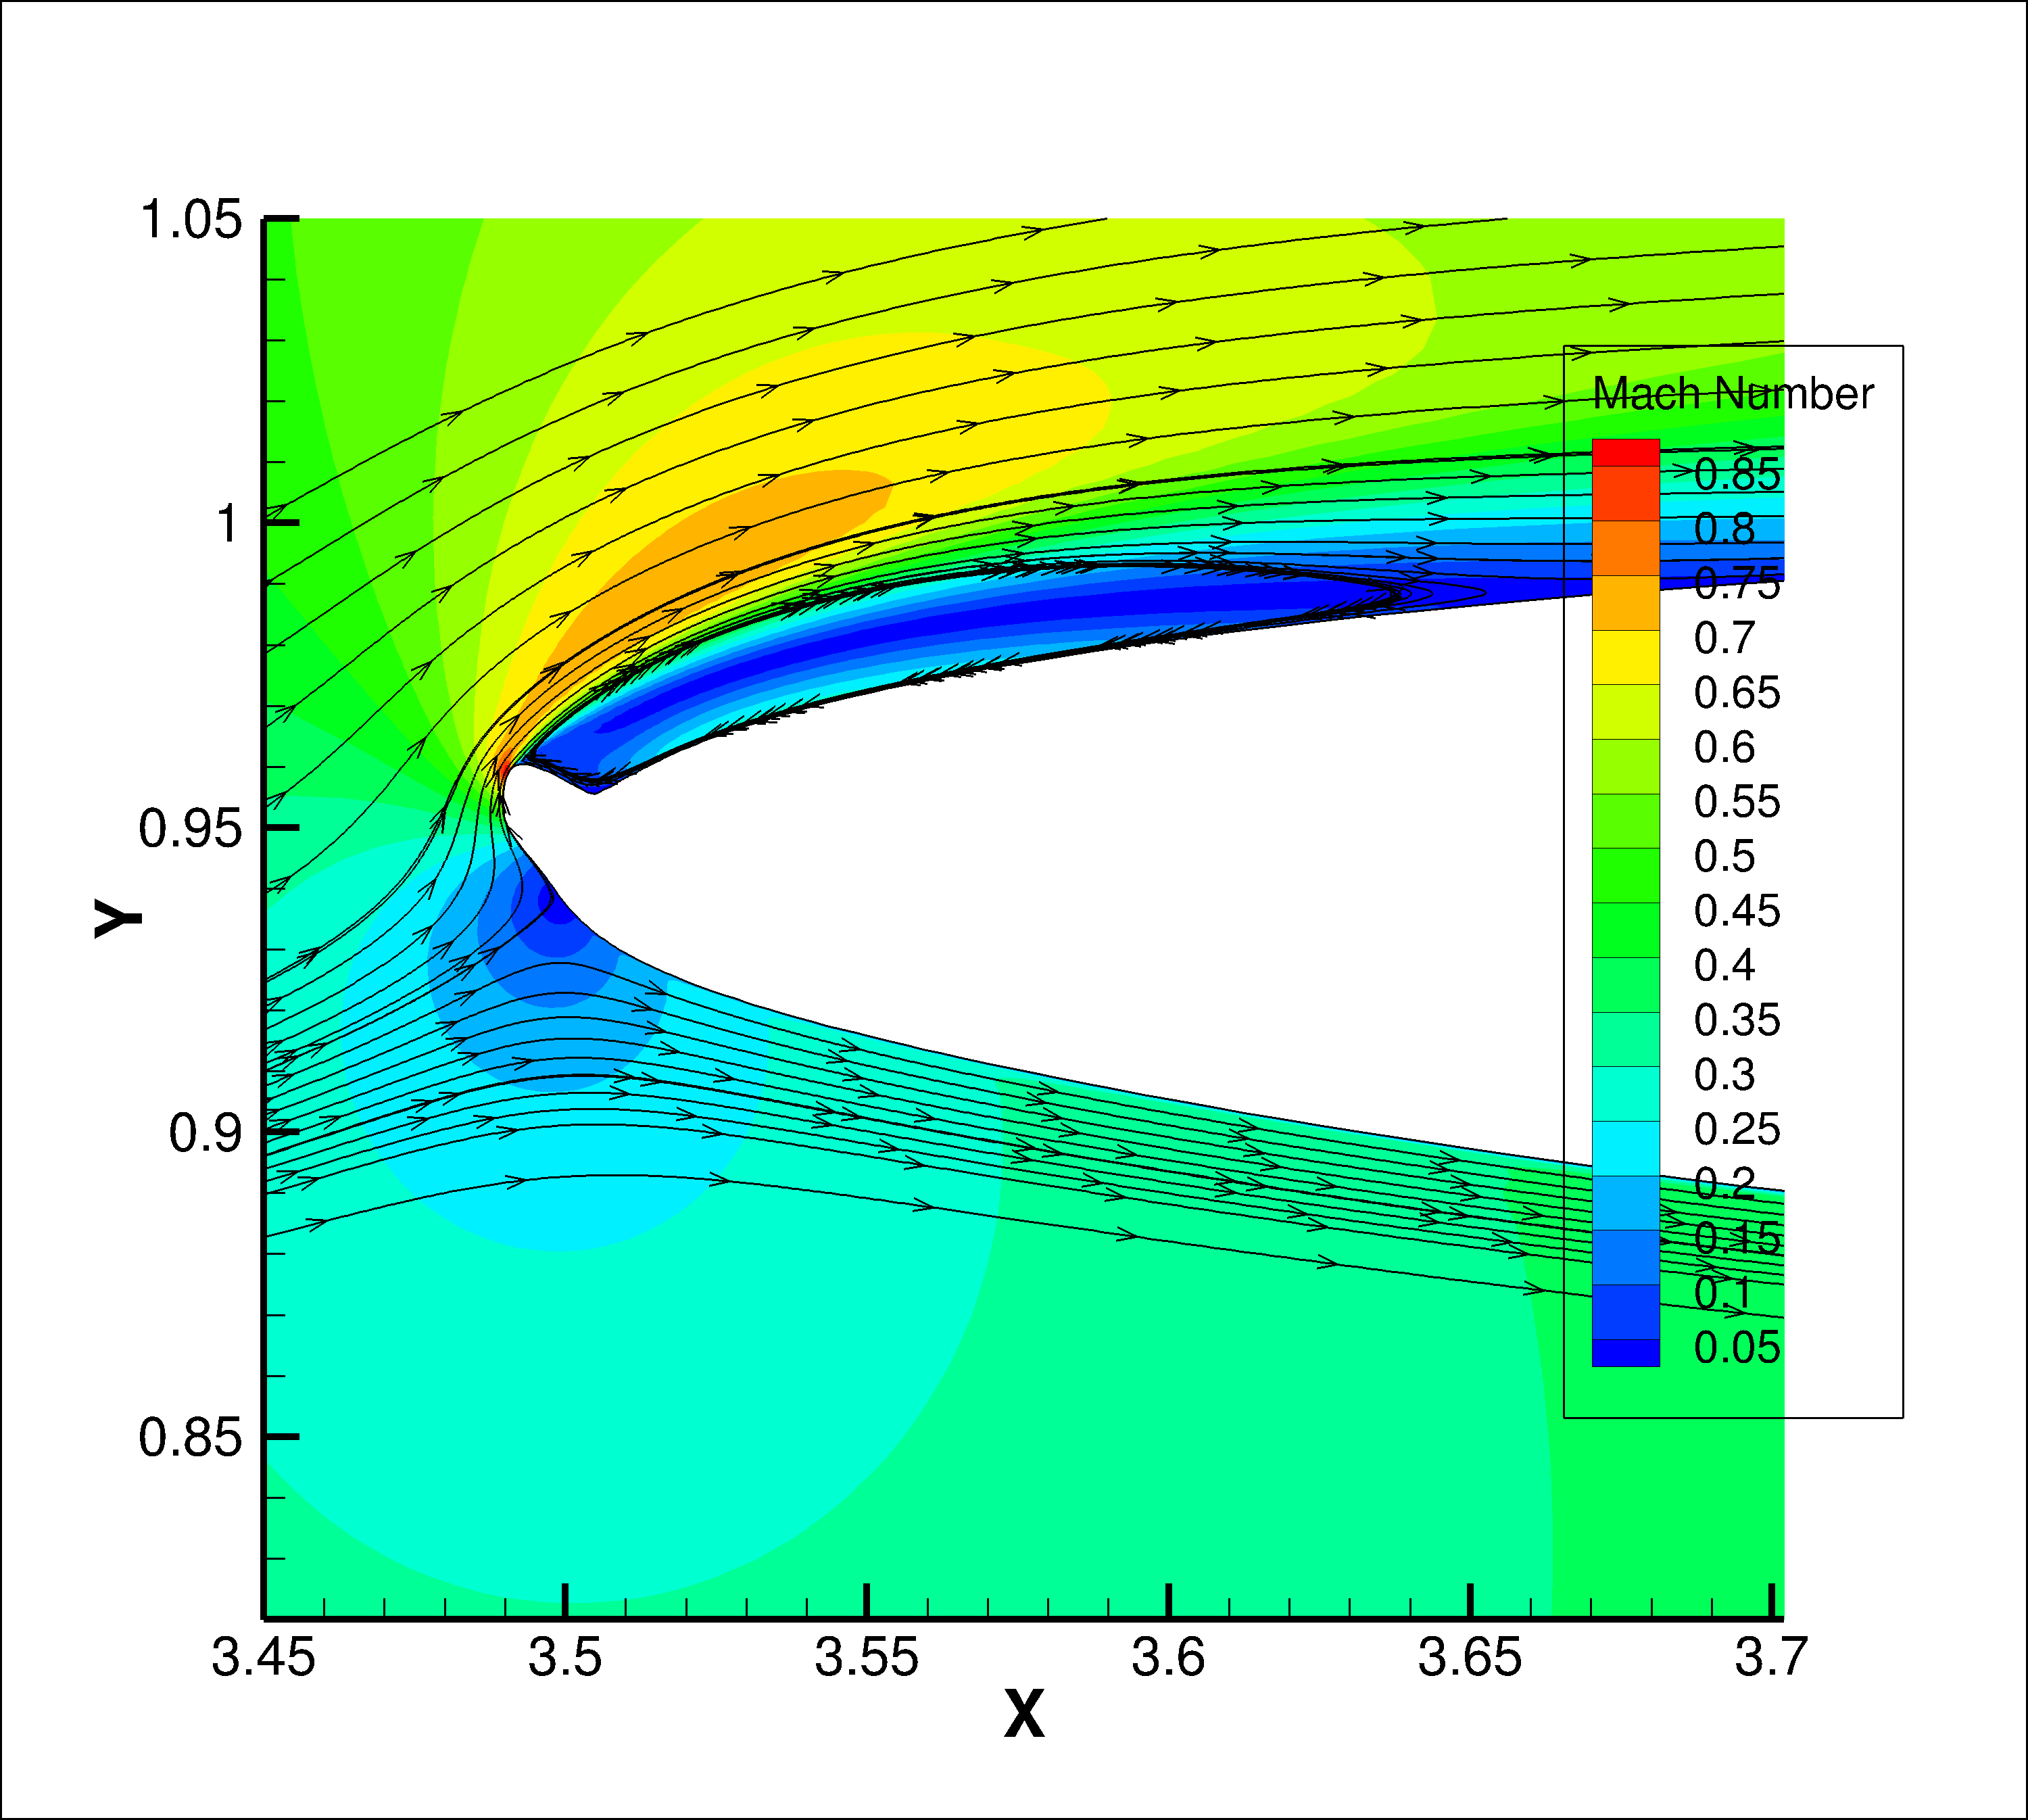
\includegraphics[width=0.4\textwidth]{BadHorn.png}
    \caption{Leading edge horn separation}
\end{figure}
\end{frame}
\begin{frame}
\frametitle{Introduction}
\label{sec-1-2}

\textbf{Significant ice shape variation, sensitivity to physical parameters}\footnote{Addy, H.E. \emph{Ice Accretions and Icing Effects for Modern Airfoils}. NASA TR 2000-210031.
 }
\begin{itemize}
\item Complex physics (aero-thermodynamics, macro/micro scale physics)
\item Uncertainty in physical parameters
\end{itemize}

\vspace*{-0.0cm}\begin{figure}
      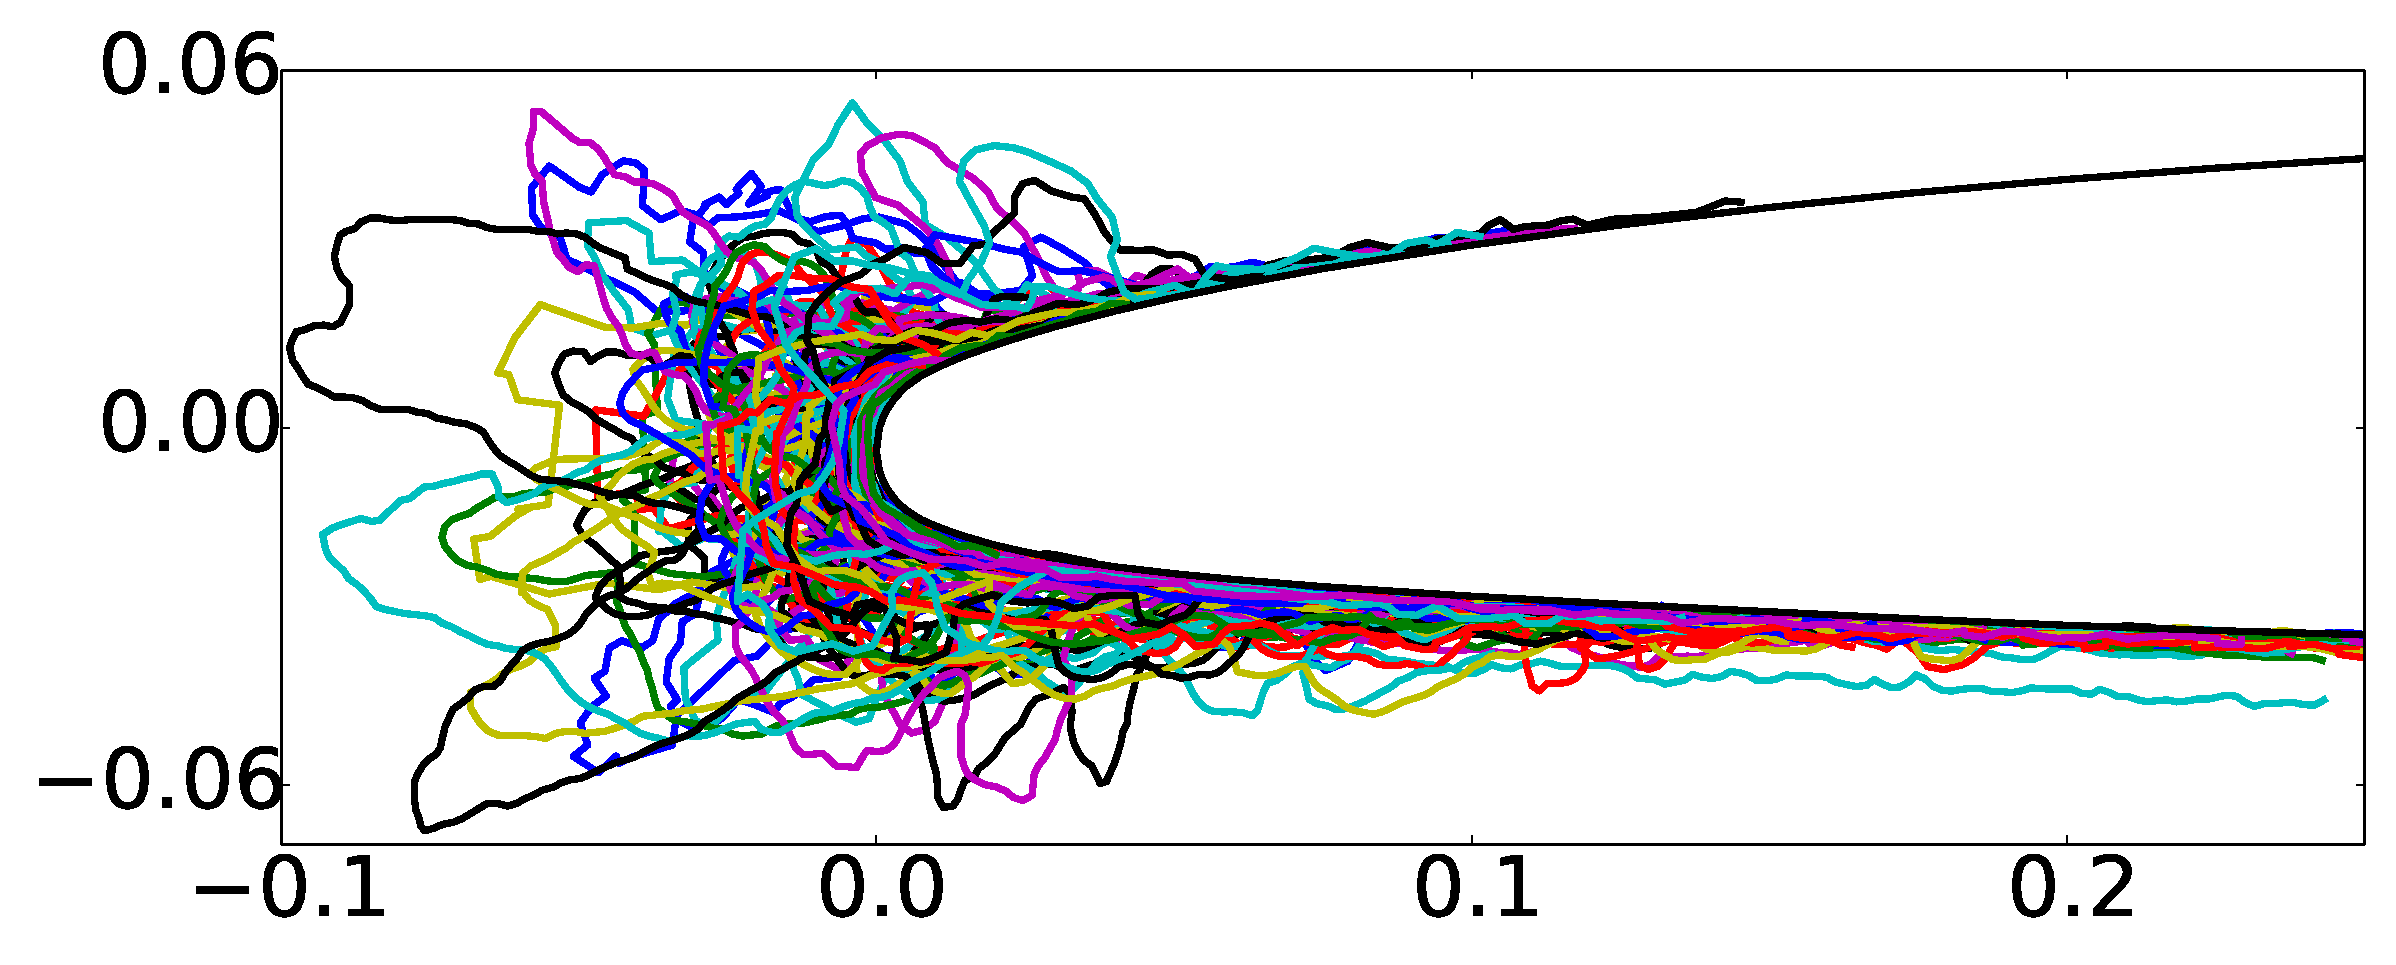
\includegraphics[width=0.75\textwidth]{GlobalDataSet}
      \caption{Wind tunnel experimental ice shapes}
\end{figure}
\end{frame}
\begin{frame}
\frametitle{Introduction}
\label{sec-1-3}

\textbf{Different types of ice accretion}\footnote{Beaugendre et. al. \emph{Development of a Second Generation In-Flight Simulation Code}. J. Fluids Engineering, 2006.
 }
\begin{itemize}
\item ``Horns'', ``ridges'', ``lobster tails'' refer to shape
\item ``Glaze'', ``rime'' refer to icing thermodynamics
\end{itemize}

\vspace*{-0.0cm}\begin{figure}
      \subfigure[Rime Ice]{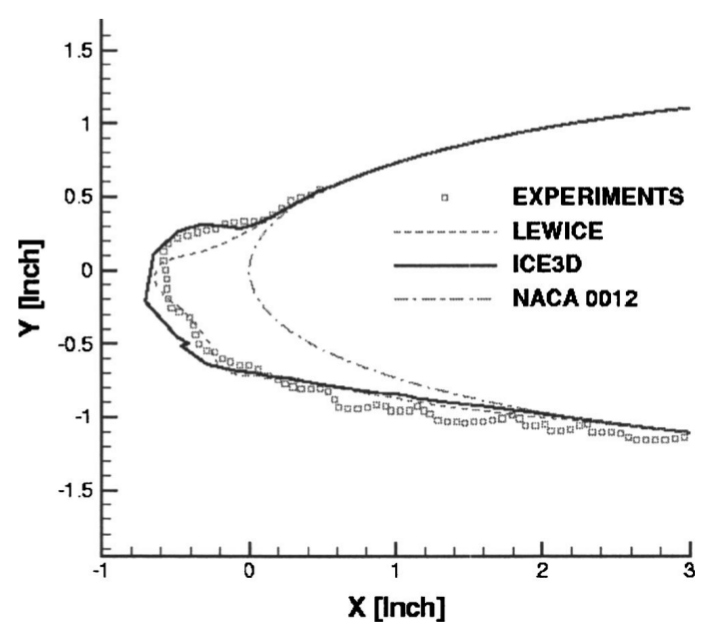
\includegraphics[width=0.4\textwidth]{Habashi2006Rime.png}}
      \subfigure[Horn Ice]{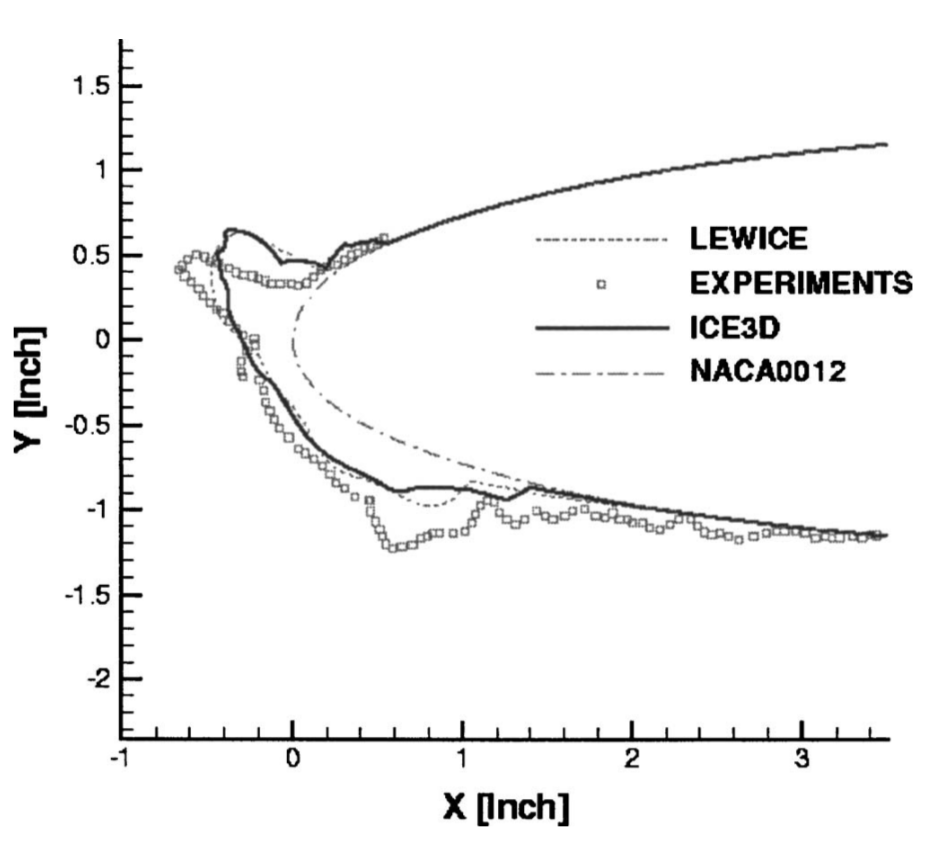
\includegraphics[width=0.4\textwidth]{Habashi2006Horn.png}}
 
\end{figure}
\end{frame}
\begin{frame}
\frametitle{Introduction}
\label{sec-1-4}

\textbf{Research Goals}
\begin{itemize}
\item Apply uncertainty quantification techniques to explore statistical
  efffects of uncertain icing parameters on ice shape and aerodynamics
\begin{itemize}
\item Polynomial chaos expansions (PCE)
\item Tensor/sparse grid collocation sampling
\item 2D steady-state RANS solver for aerodynamic assessment
\end{itemize}
\item Build ice shape model from data
\begin{itemize}
\item Aggregate ice shape database
\item Cluster shapes using spectral graph partitioning
\item Model shape variation using Proper Orthogonal Decomposition (POD)
\end{itemize}
\item Quantify effects of physical uncertainties in aero-thermodynamics
\begin{itemize}
\item Build a computational ice-accretion code
\item UQ on governing parameters (LWC, temperature, accretion time, etc.)
\end{itemize}
\end{itemize}
\end{frame}
\begin{frame}
\frametitle{Introduction}
\label{sec-1-5}

\textbf{Thesis Structure}
\begin{itemize}
\item Heuristic UQ
\begin{itemize}
\item Ice shape scaling parameters
\item Verify PCE techniques against Monte Carlo simulations
\end{itemize}
\item Data-based UQ
\begin{itemize}
\item Build ice shape model from data
\item Clustering + POD
\end{itemize}
\item Computational UQ
\begin{itemize}
\item Build computational ice accretion code
\item Droplet impingement + thermodynamic PDE solvers
\end{itemize}
\end{itemize}
\end{frame}
\section{Heuristic UQ}
\label{sec-2}
\begin{frame}
\frametitle{Canonical Ice Shapes}
\label{sec-2-1}

\begin{itemize}
\item \textbf{Basic ice shapes}\footnote{Papadakis et. al. \emph{Aerodynamic Scaling Experiments with Simulated Ice Accretions}. AIAA 2001-0833.
 }
\end{itemize}
\centering
\vspace{-0.5cm}
\begin{minipage}[t]{0.4\linewidth}
\begin{figure}[t]
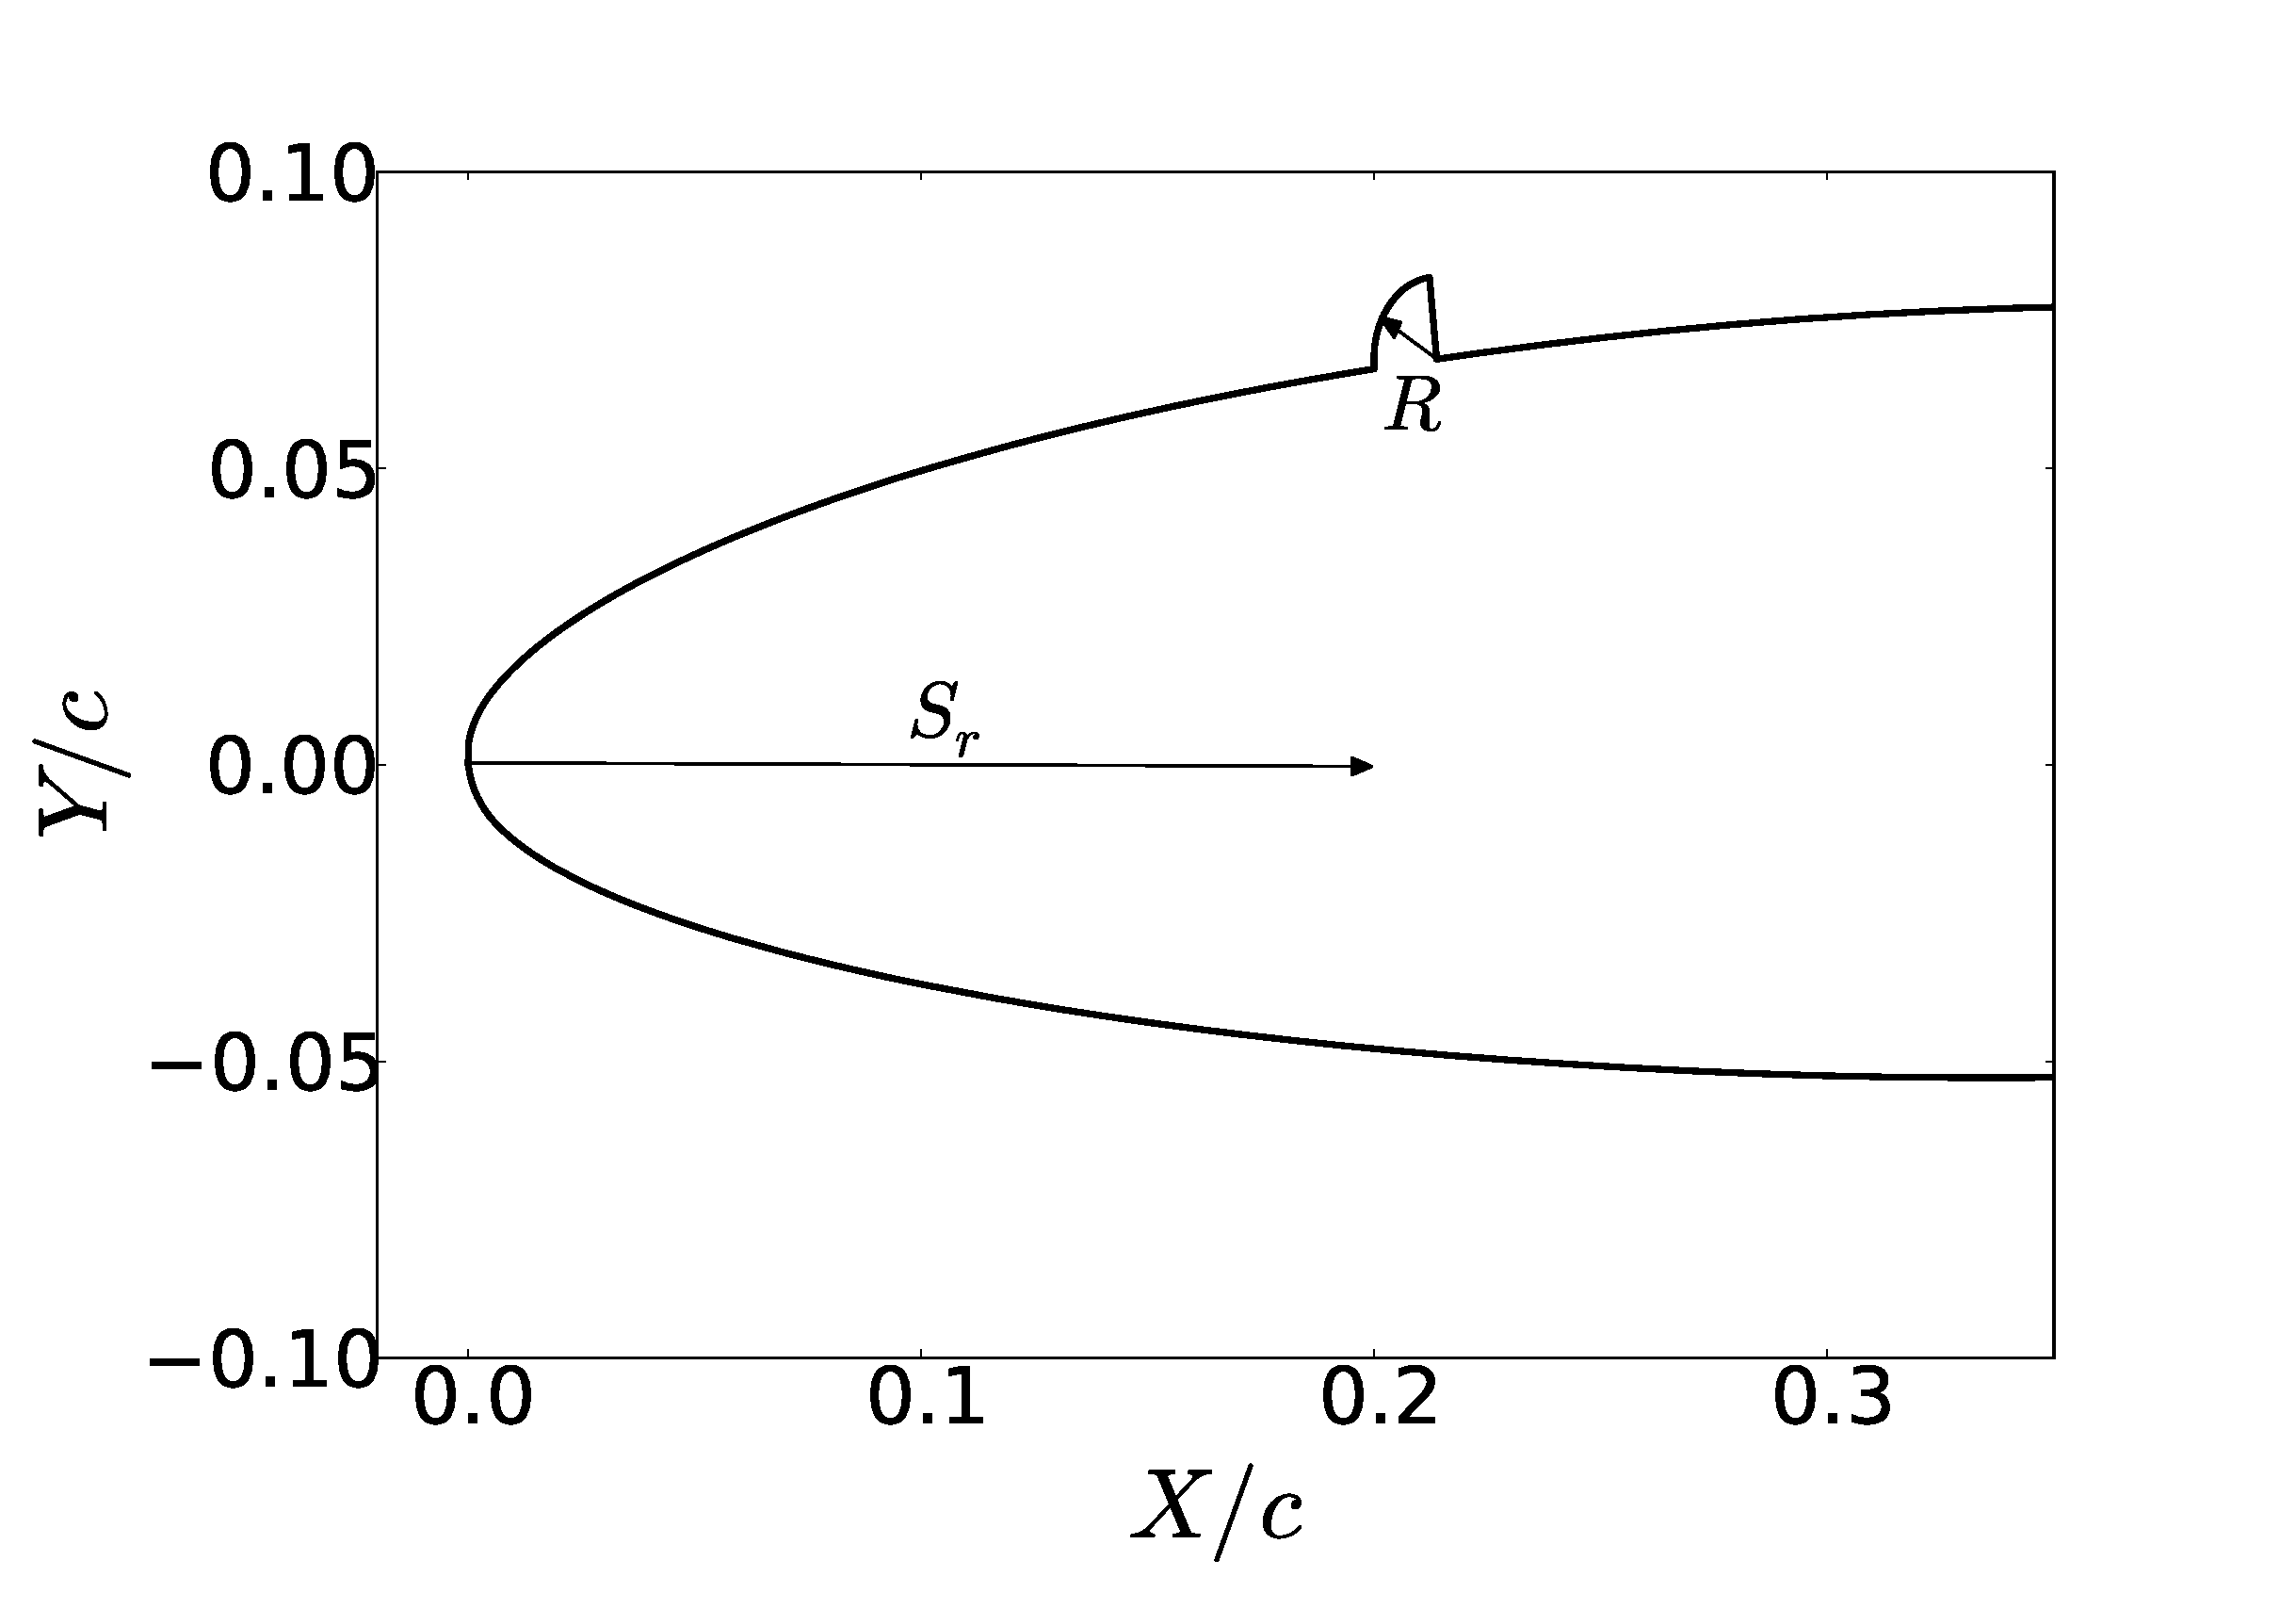
\includegraphics[width=0.95\textwidth]{RidgeParameters}
\caption{Ridge Ice}
\end{figure}
\vspace{-0.5cm}
\begin{itemize}
\item Forms aft of deicing mechanism
\item Runback water refreezes to form step
\end{itemize}
\end{minipage}
\begin{minipage}[t]{0.4\linewidth}
\begin{figure}[t]
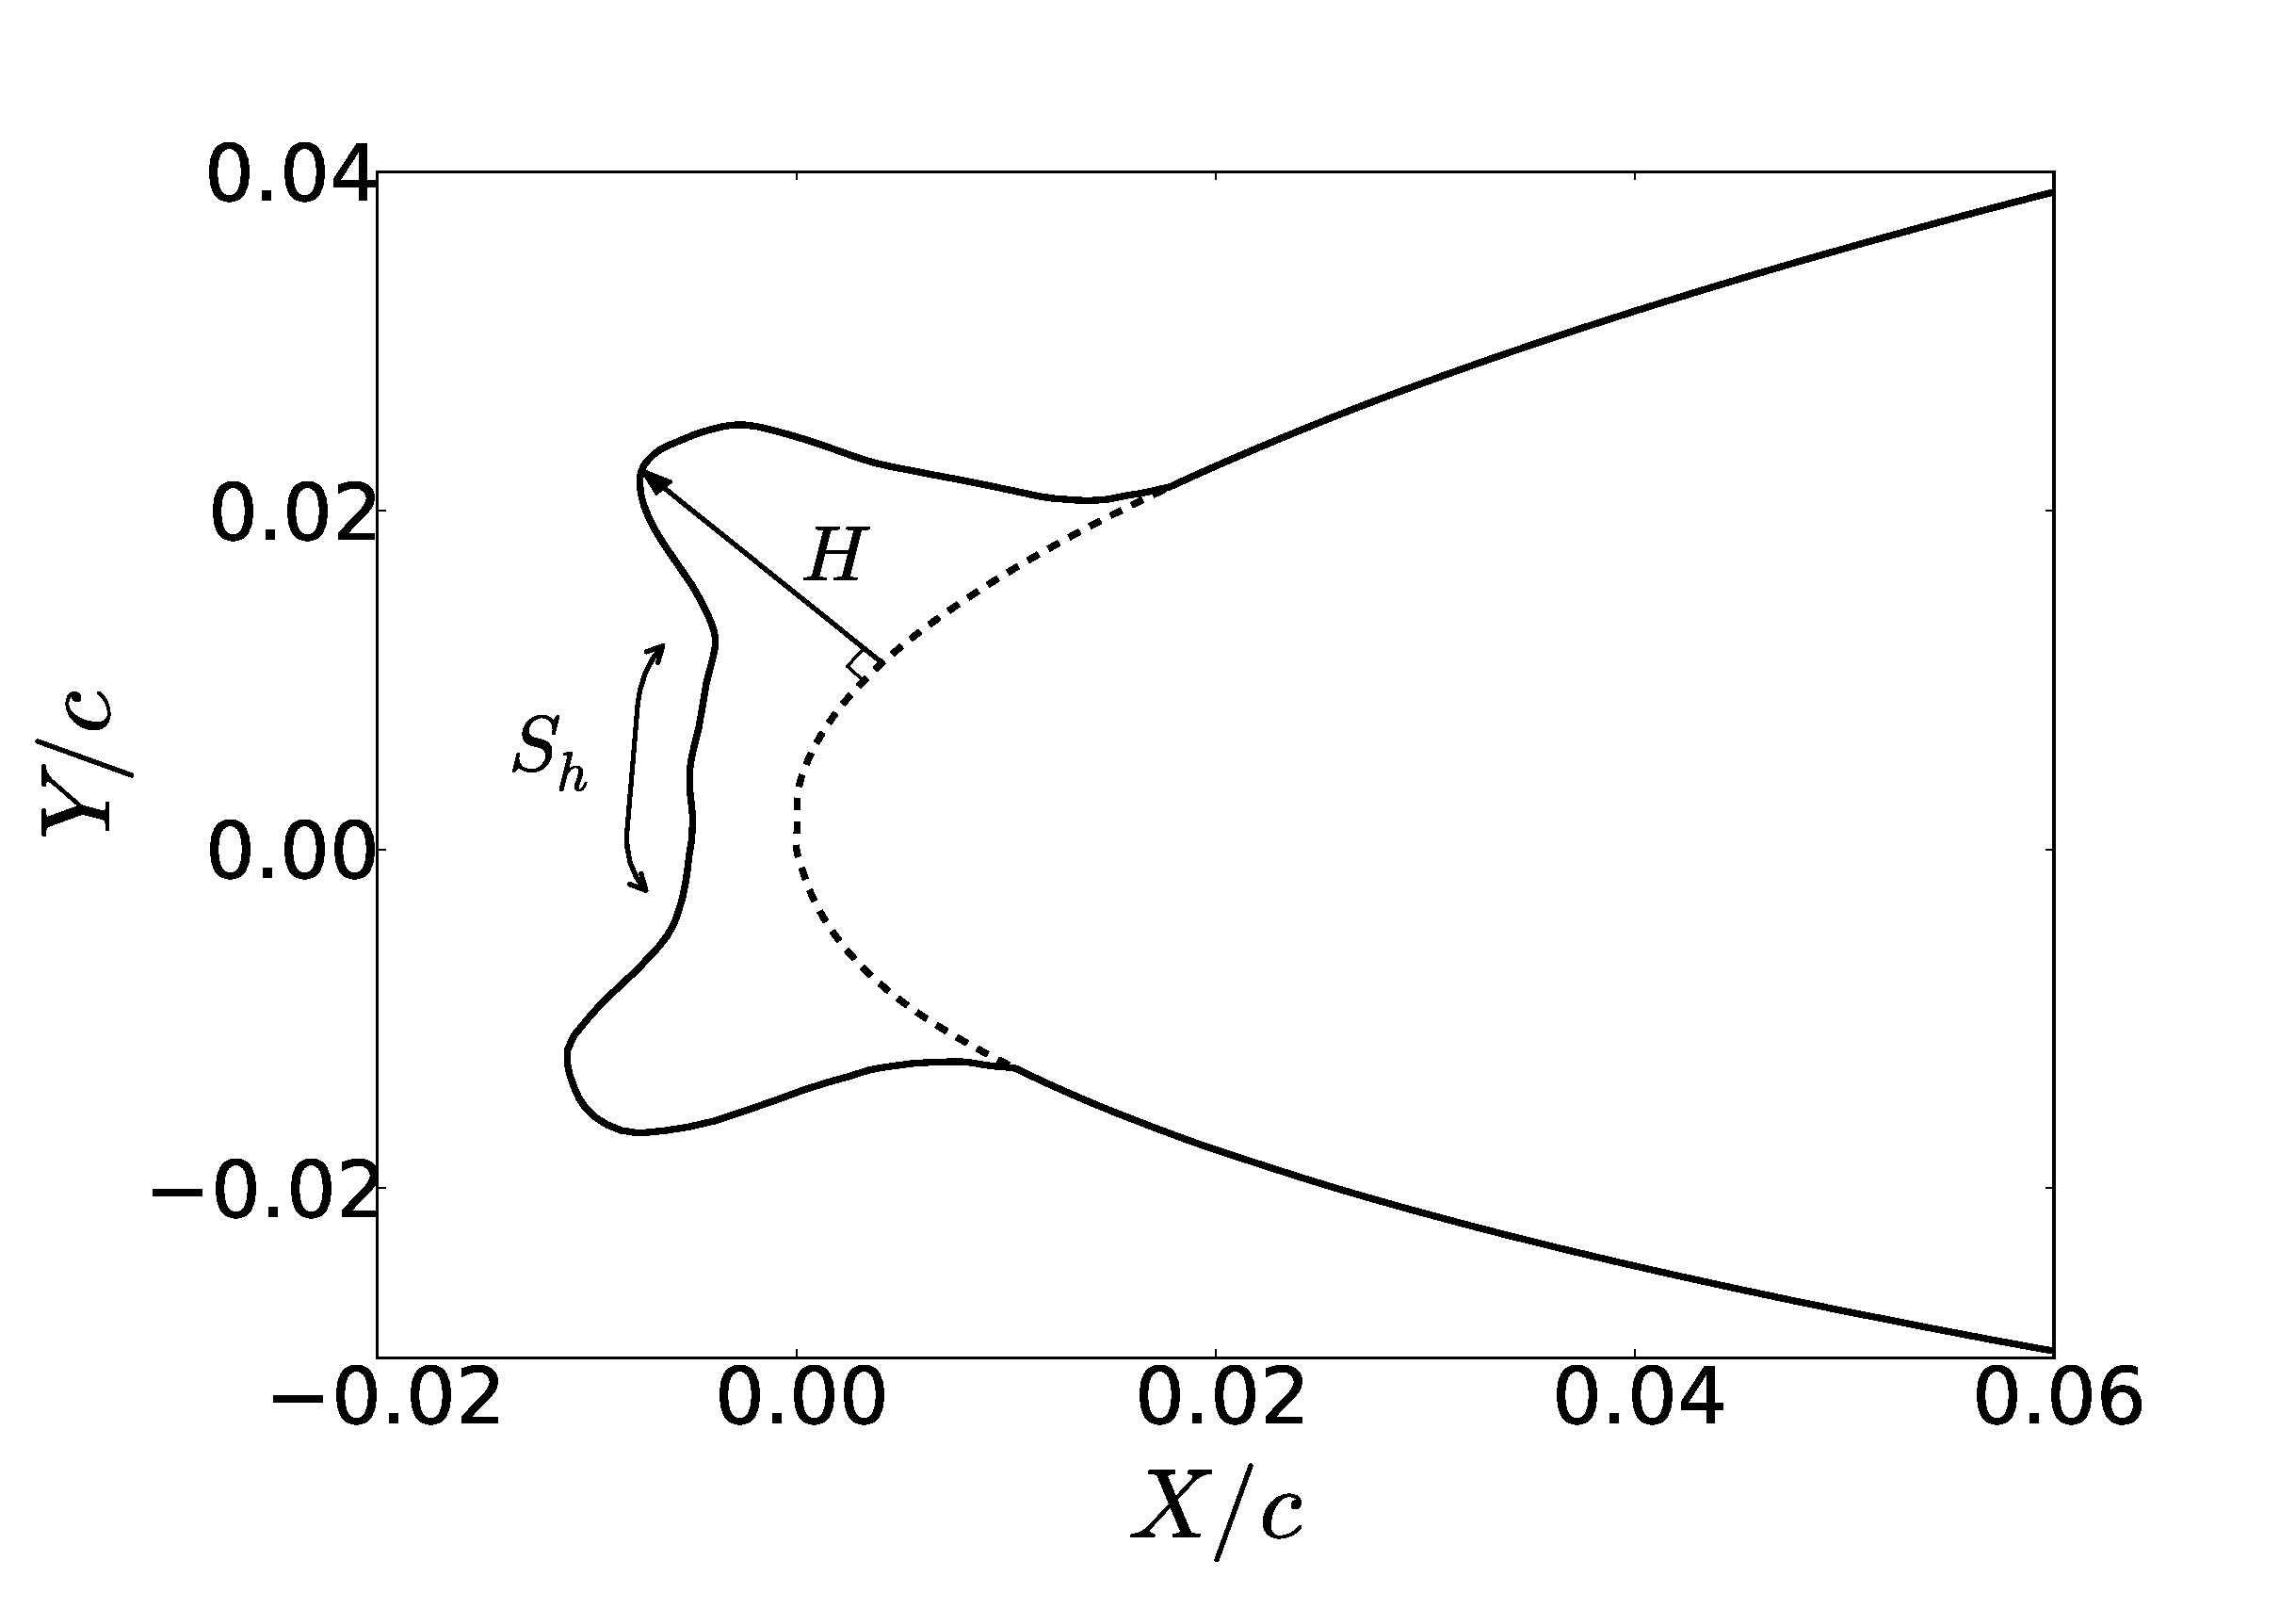
\includegraphics[width=0.95\textwidth]{NominalHorn}
\caption{Horn Ice}
\end{figure}
\vspace{-0.5cm}
\begin{itemize}
\item Forms in relatively warm conditions
\item Differential heat transfer rate
\end{itemize}
\end{minipage}
\end{frame}
\begin{frame}
\frametitle{Canonical Ice Shapes}
\label{sec-2-2}

\begin{itemize}
\item \textbf{Basic scalings/translations}\footnote{DeGennaro A., Rowley C.W., and Martinelli,
L. \emph{Uncertainty Quantification for Airfoil Icing using Polynomial Chaos Expansions}. Journal of Aircraft, 2015.
 }
\end{itemize}
\centering
\vspace{-0.5cm}
\begin{minipage}[t]{0.45\linewidth}
\begin{figure}[t]
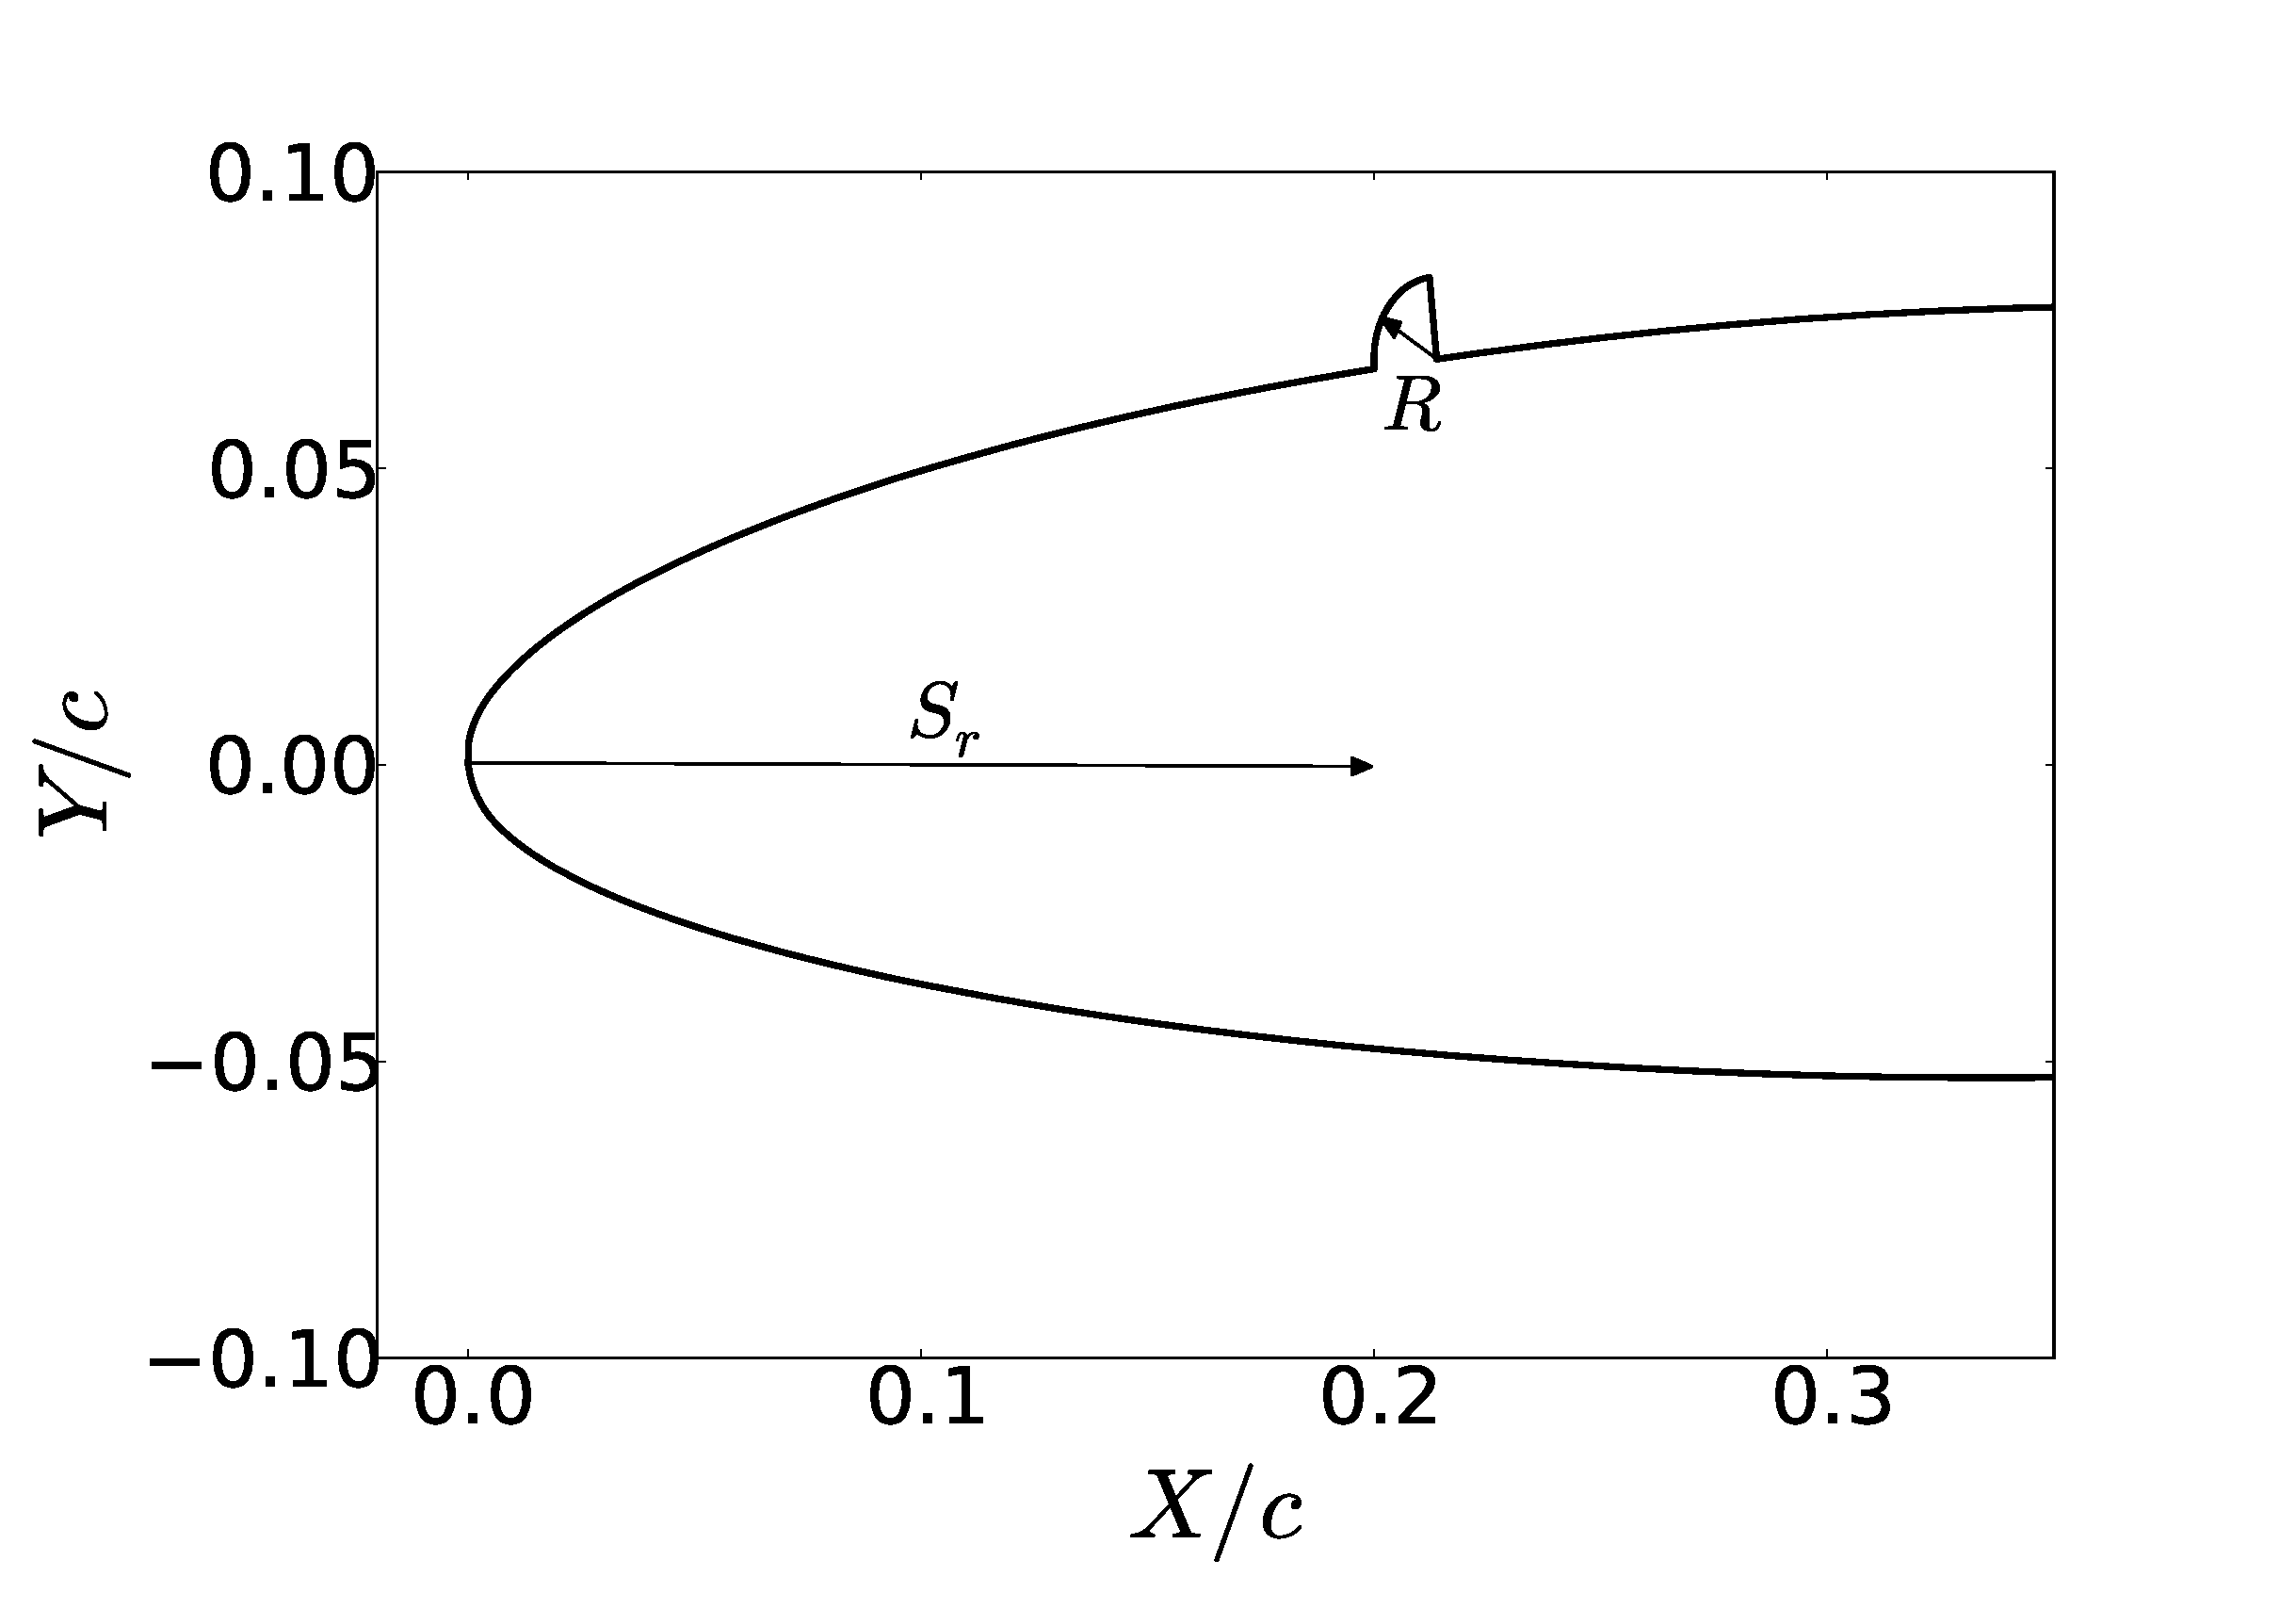
\includegraphics[width=0.95\textwidth]{RidgeParameters}
\caption{Ridge Parameterization}
\end{figure}
\vspace{-0.5cm}
\begin{itemize}
\item Ridge radius
\item Ridge position
\end{itemize}
\end{minipage}
\begin{minipage}[t]{0.45\linewidth}
\begin{figure}[t]
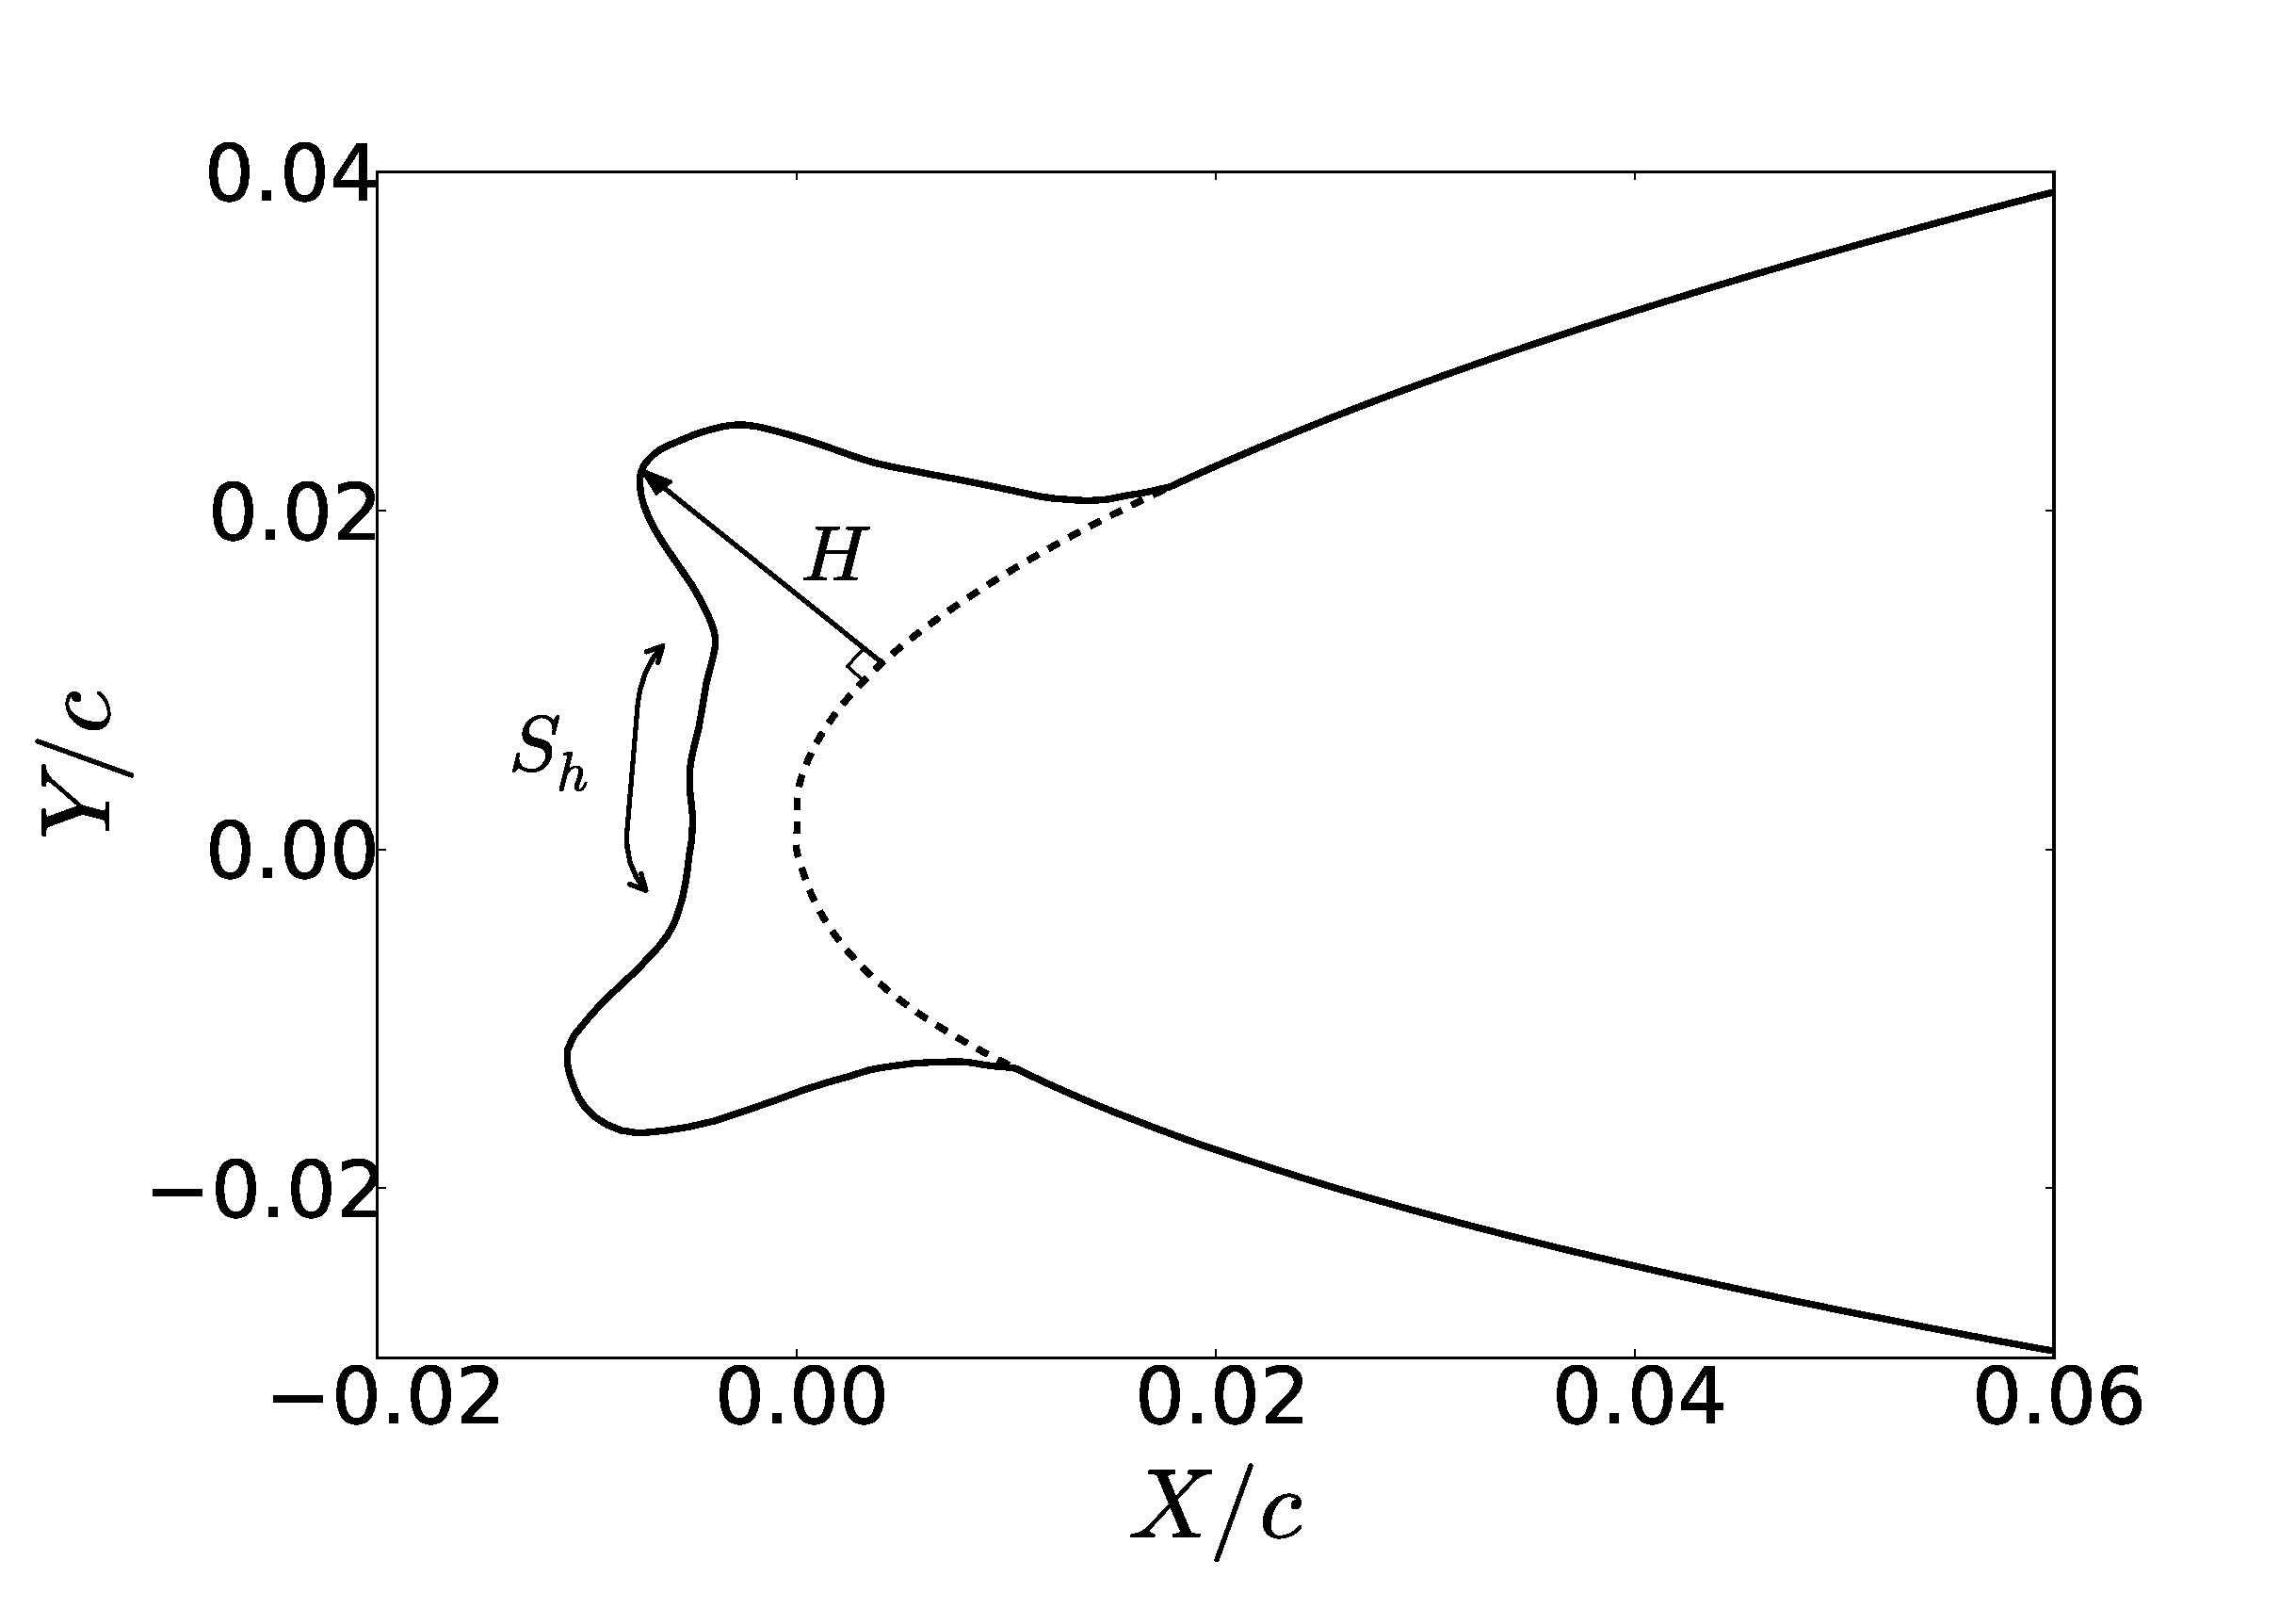
\includegraphics[width=0.95\textwidth]{NominalHorn}
\caption{Horn Parameterization}
\end{figure}
\vspace{-0.5cm}
\begin{itemize}
\item Horn height
\item Horn separation
\end{itemize}
\end{minipage}
\end{frame}
\begin{frame}
\frametitle{Application to Icing UQ}
\label{sec-2-3}

\begin{itemize}
\item We wish to apply a fast and accurate method for quantifying
  uncertainty in the aerodynamics of these ice shapes
\item Choose to use polynomial chaos expansions (PCE)
\begin{itemize}
\item Fast compared to Monte Carlo
\item Explicit surrogate
\item Easy statistical sampling
\item Can compute sensitivities, analysis of variance
\end{itemize}
\item We will compute UQ results for horn and ridge problems using PCE,
  and verify them against high-resolution Monte Carlo simulations
\end{itemize}
\end{frame}
\begin{frame}
\frametitle{Polynomial Chaos Expansions (PCE)}
\label{sec-2-4}


\begin{itemize}
\item \textbf{Polynomial Chaos Framework} \footnote{Xiu D. \emph{Numerical Methods for Stochastic Computations: A Spectral Method Approach}. Princeton University Press, 2010.
 }
\begin{itemize}
\item Let $\bv{Z} = (Z_1 \ldots Z_d)$ be $d$ random variables with PDF
    $\rho(\bv{Z})$ that parameterize ice
\item Let $\lbrace \Phi_k \rbrace$ denote the set of polynomials
    which are orthogonal w.r.t. $\rho(\bv{Z})$
\item Let $y(\bv{Z})$ denote the mapping from $\bv{Z}$ to an aerodynamic
    performance metric
\end{itemize}
\item \textbf{Probabilistic Collocation Method:}
\begin{itemize}
\item \emph{Representation} 
    \begin{equation*}
      y(\bv{Z}) \approx \sum_{|i|=0}^N y_i \Phi_i(\bv{Z})
    \end{equation*}
\item \emph{Orthonormality} 
    \begin{equation*}
    \begin{aligned}
      \ip{f}{g} &= \int_{\Gamma} f(\bv{z})g(\bv{z}) \rho(\bv{z}) d\bv{z} \\
      \ip{\Phi_i}{\Phi_j} &= \delta_{ij}
    \end{aligned}
    \end{equation*}
\item \emph{Quadrature} 
    \begin{equation*}
      y_k = \ip{y}{\Phi_k} \approx \sum_{i=0}^{Q}
    y(\bv{Z}^{(k)}) \Phi_k(\bv{Z}^{(k)}) w_k
    \end{equation*}
\end{itemize}
\end{itemize}
\end{frame}
\begin{frame}
\frametitle{PCE Collocation}
\label{sec-2-5}

\begin{columns}[c]
  \column{0.7\textwidth}
    \centering
    \begin{figure}
    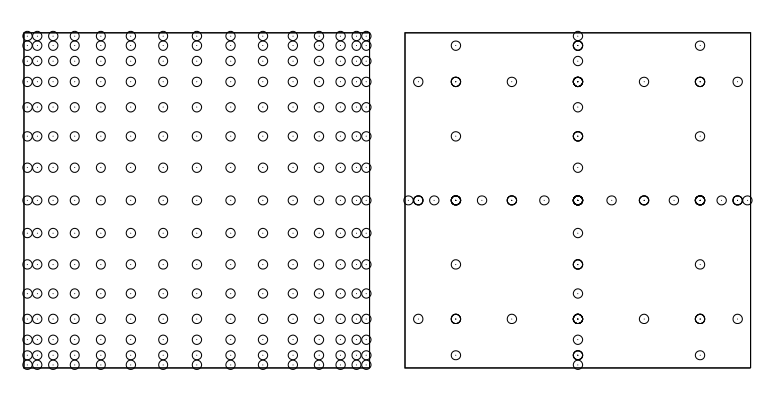
\includegraphics[width=0.95\textwidth]{SparseGrid1}
    \caption{Full Tensor Product vs. Sparse Grid}
    \end{figure}
  \column{0.3\textwidth}
    \centering
    \begin{figure}
    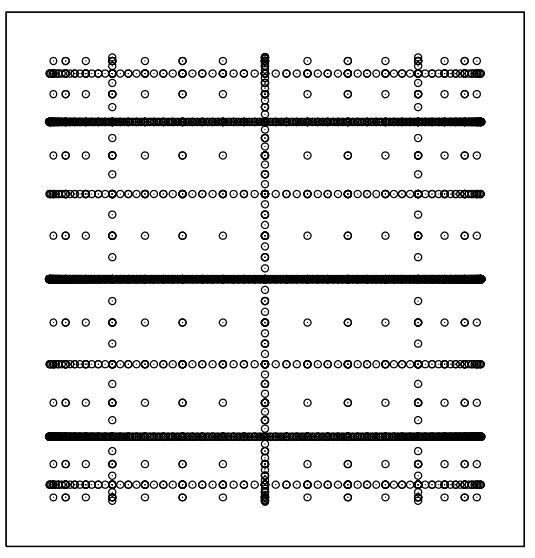
\includegraphics[width=0.95\textwidth]{SparseGrid2} \\
    \caption{Anisotropic Grid}
    \end{figure}
\end{columns}

\begin{itemize}
\item Full tensor grids can be used when probability space is low-dimensional
\item Sparse grids can be used otherwise\footnote{LeMaitre O. \emph{Spectral Methods for Uncertainty Quantification}. Springer, 2010.
 }
\end{itemize}
\end{frame}
\begin{frame}
\frametitle{Application to Icing UQ}
\label{sec-2-6}

\begin{itemize}
\item Parameterize shape variation for ridge/horn
\begin{itemize}
\item 2 parameters, equip with a distribution
\end{itemize}
\item Apply polynomial chaos methodology
\begin{itemize}
\item Full tensor grid sampling
\item 4$^{th}$-order polynomials --> $5\times5$ collocation mesh
\end{itemize}
\item Compute aerodynamics of resulting shapes
\begin{itemize}
\item In-house 2D steady-state RANS solver + hyperbolic mesh generator
\end{itemize}
\item Compare results against 500 Quasi-Monte Carlo samples
\end{itemize}
\end{frame}
\begin{frame}
\frametitle{Ridge Study}
\label{sec-2-7}

\centering
\vspace{-0.5cm}
\begin{minipage}[t]{0.45\linewidth}
\begin{figure}[t]
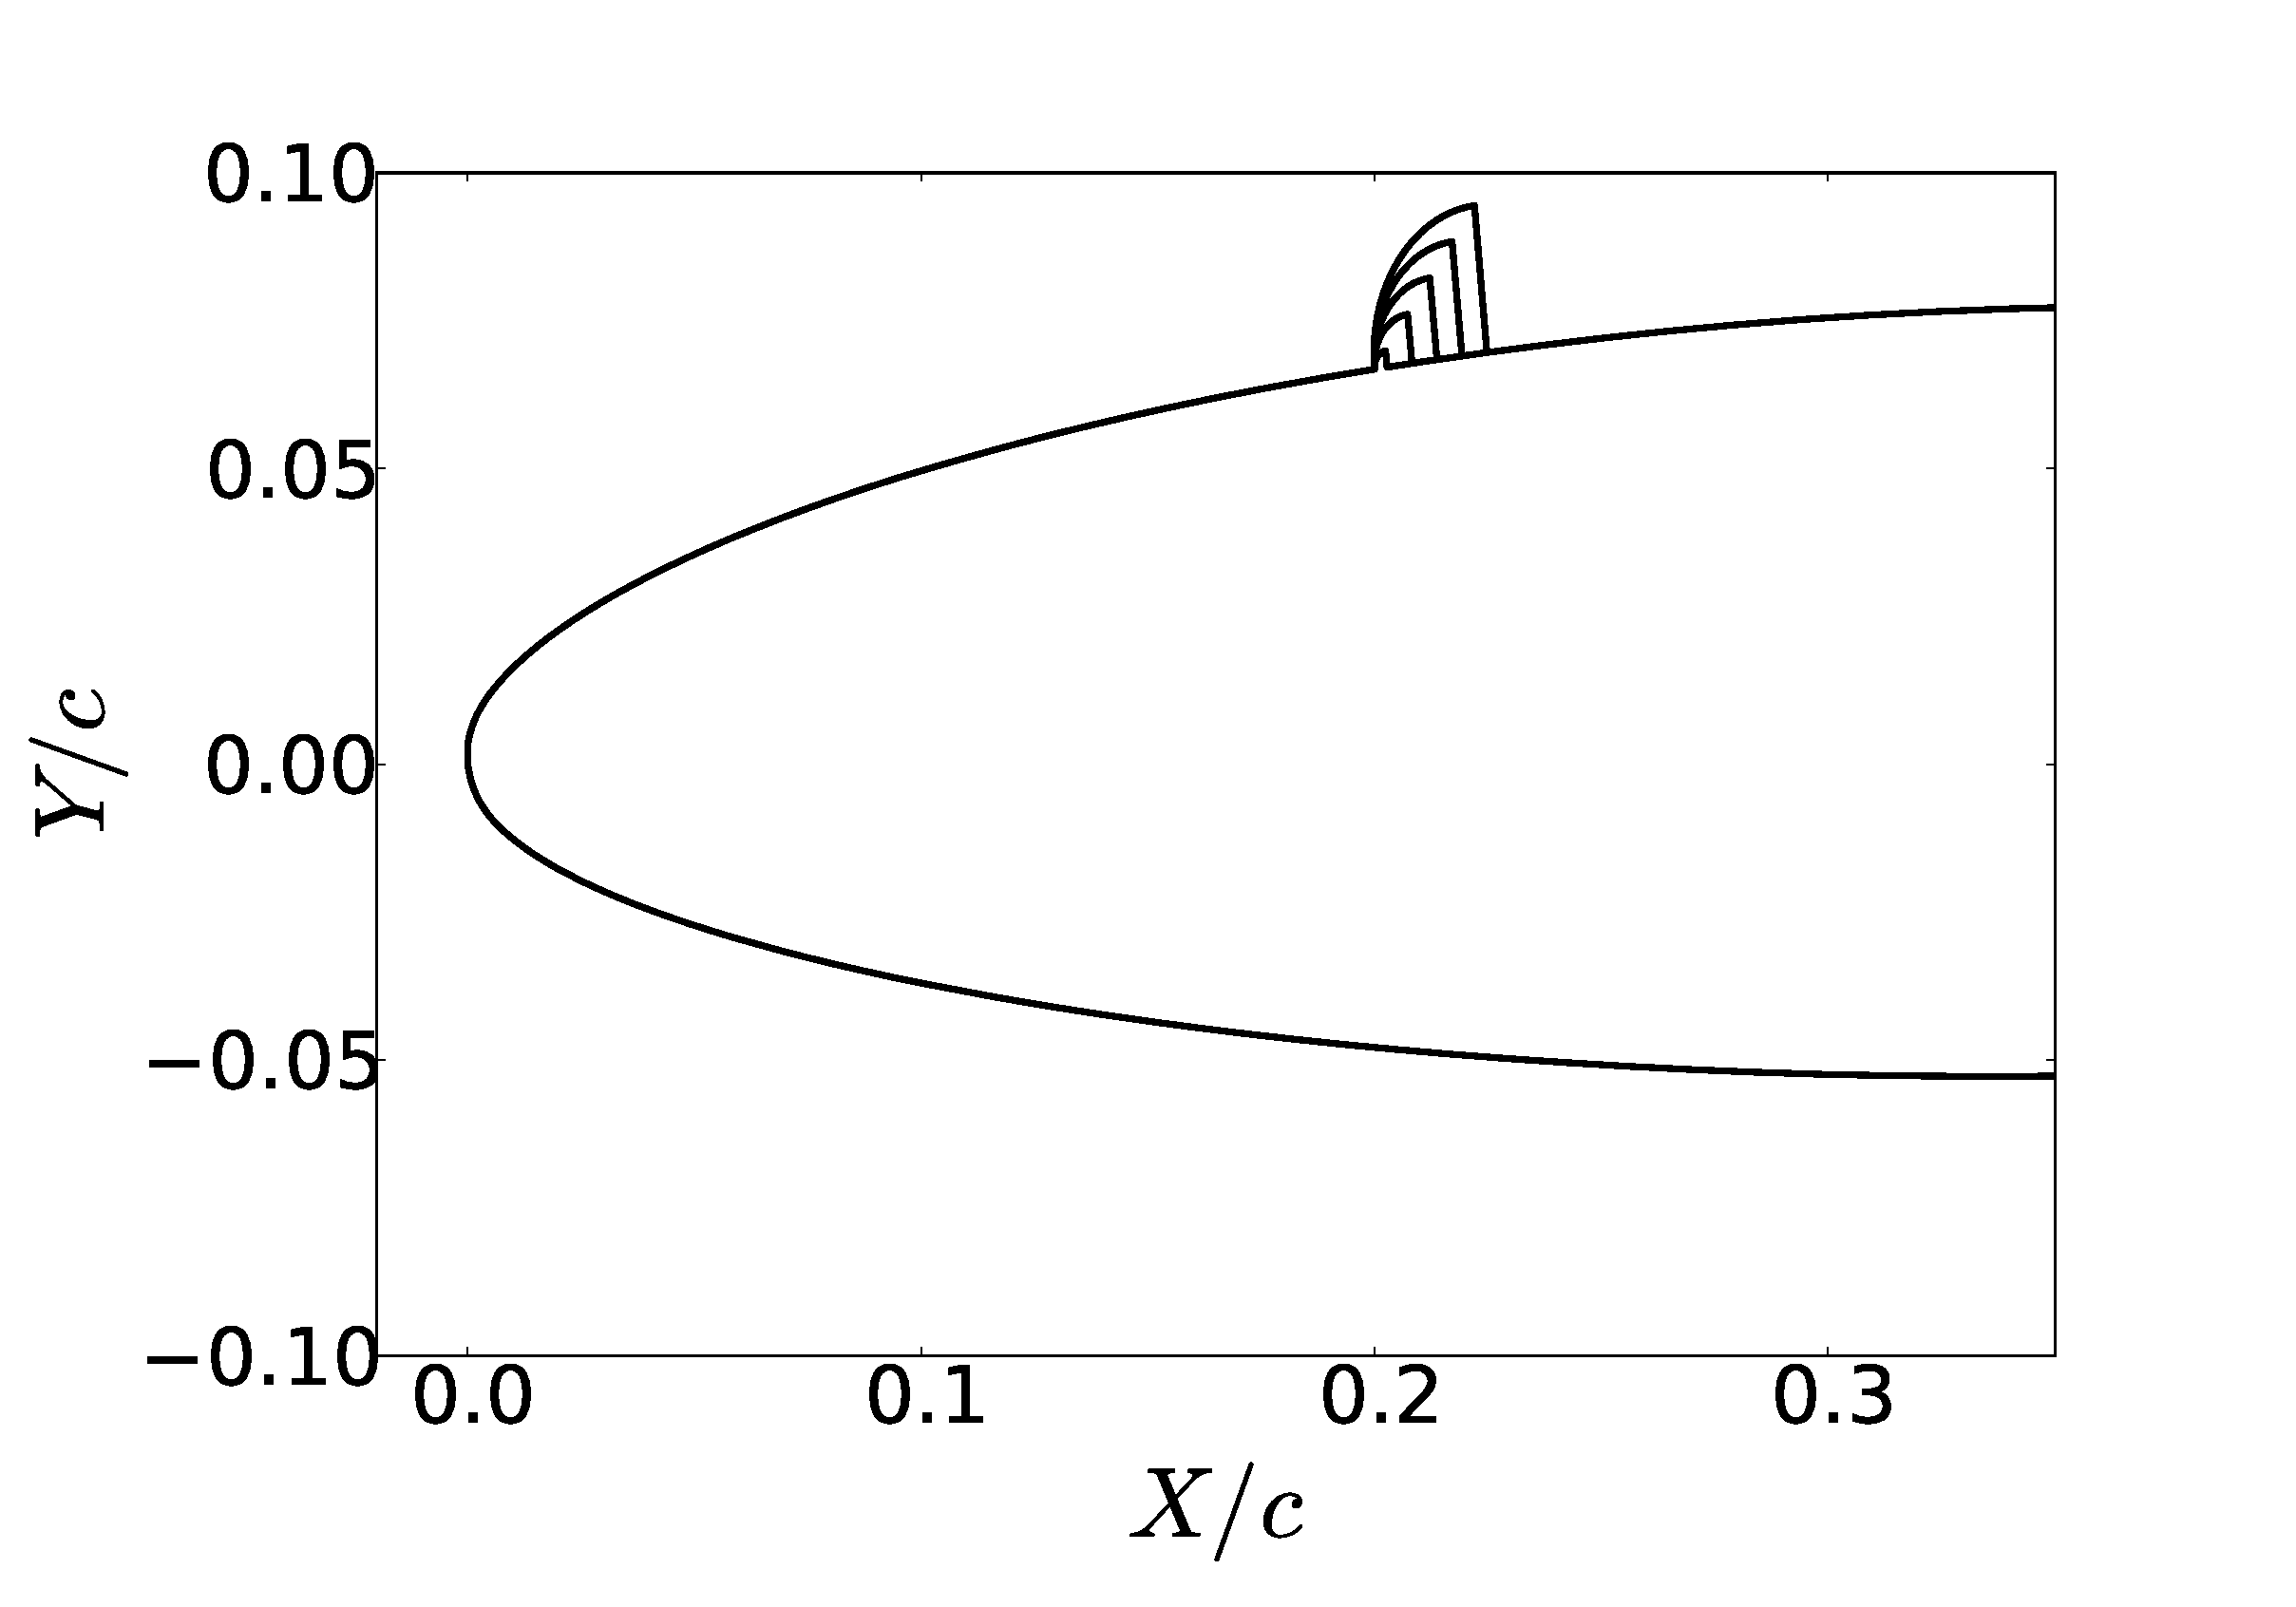
\includegraphics[width=0.75\textwidth]{RidgeRVariation}
\end{figure}
\vspace{-0.5cm}
\begin{figure}[t]
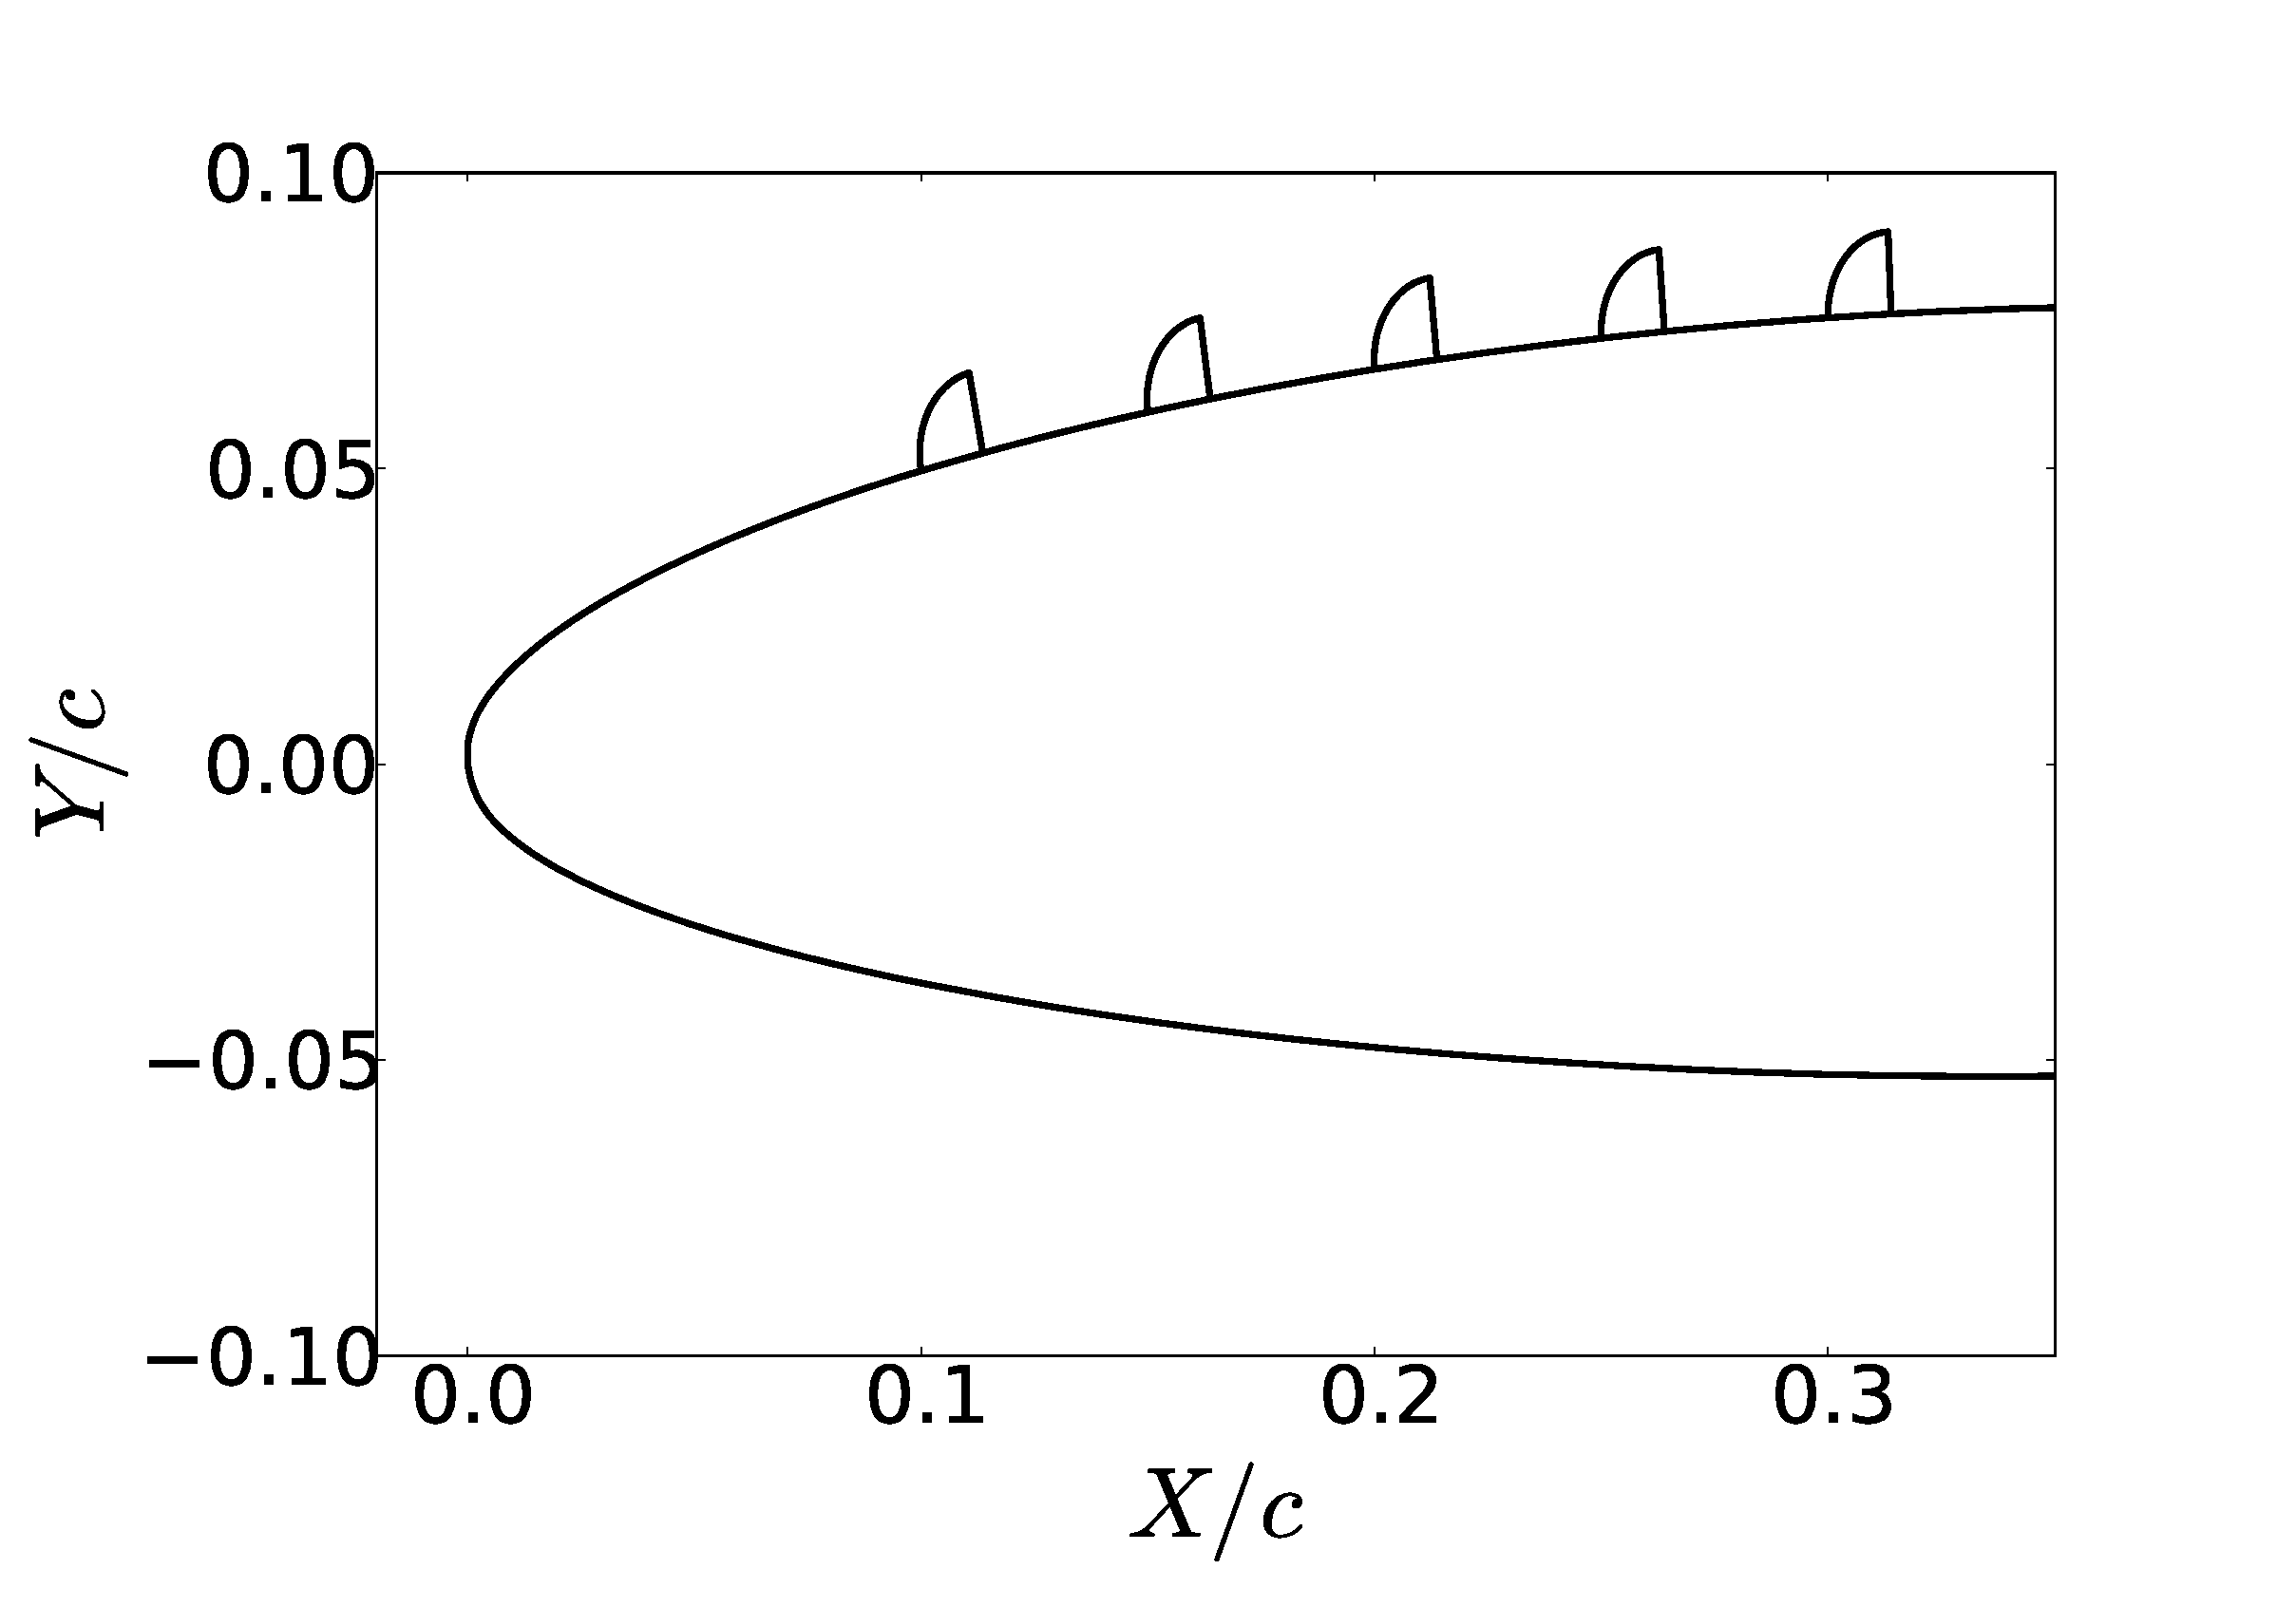
\includegraphics[width=0.75\textwidth]{RidgeSVariation}
\caption{Ridge Variations}
\end{figure}
\vspace{-0.5cm}
\end{minipage}
\begin{minipage}[t]{0.45\linewidth}
\begin{figure}[t]
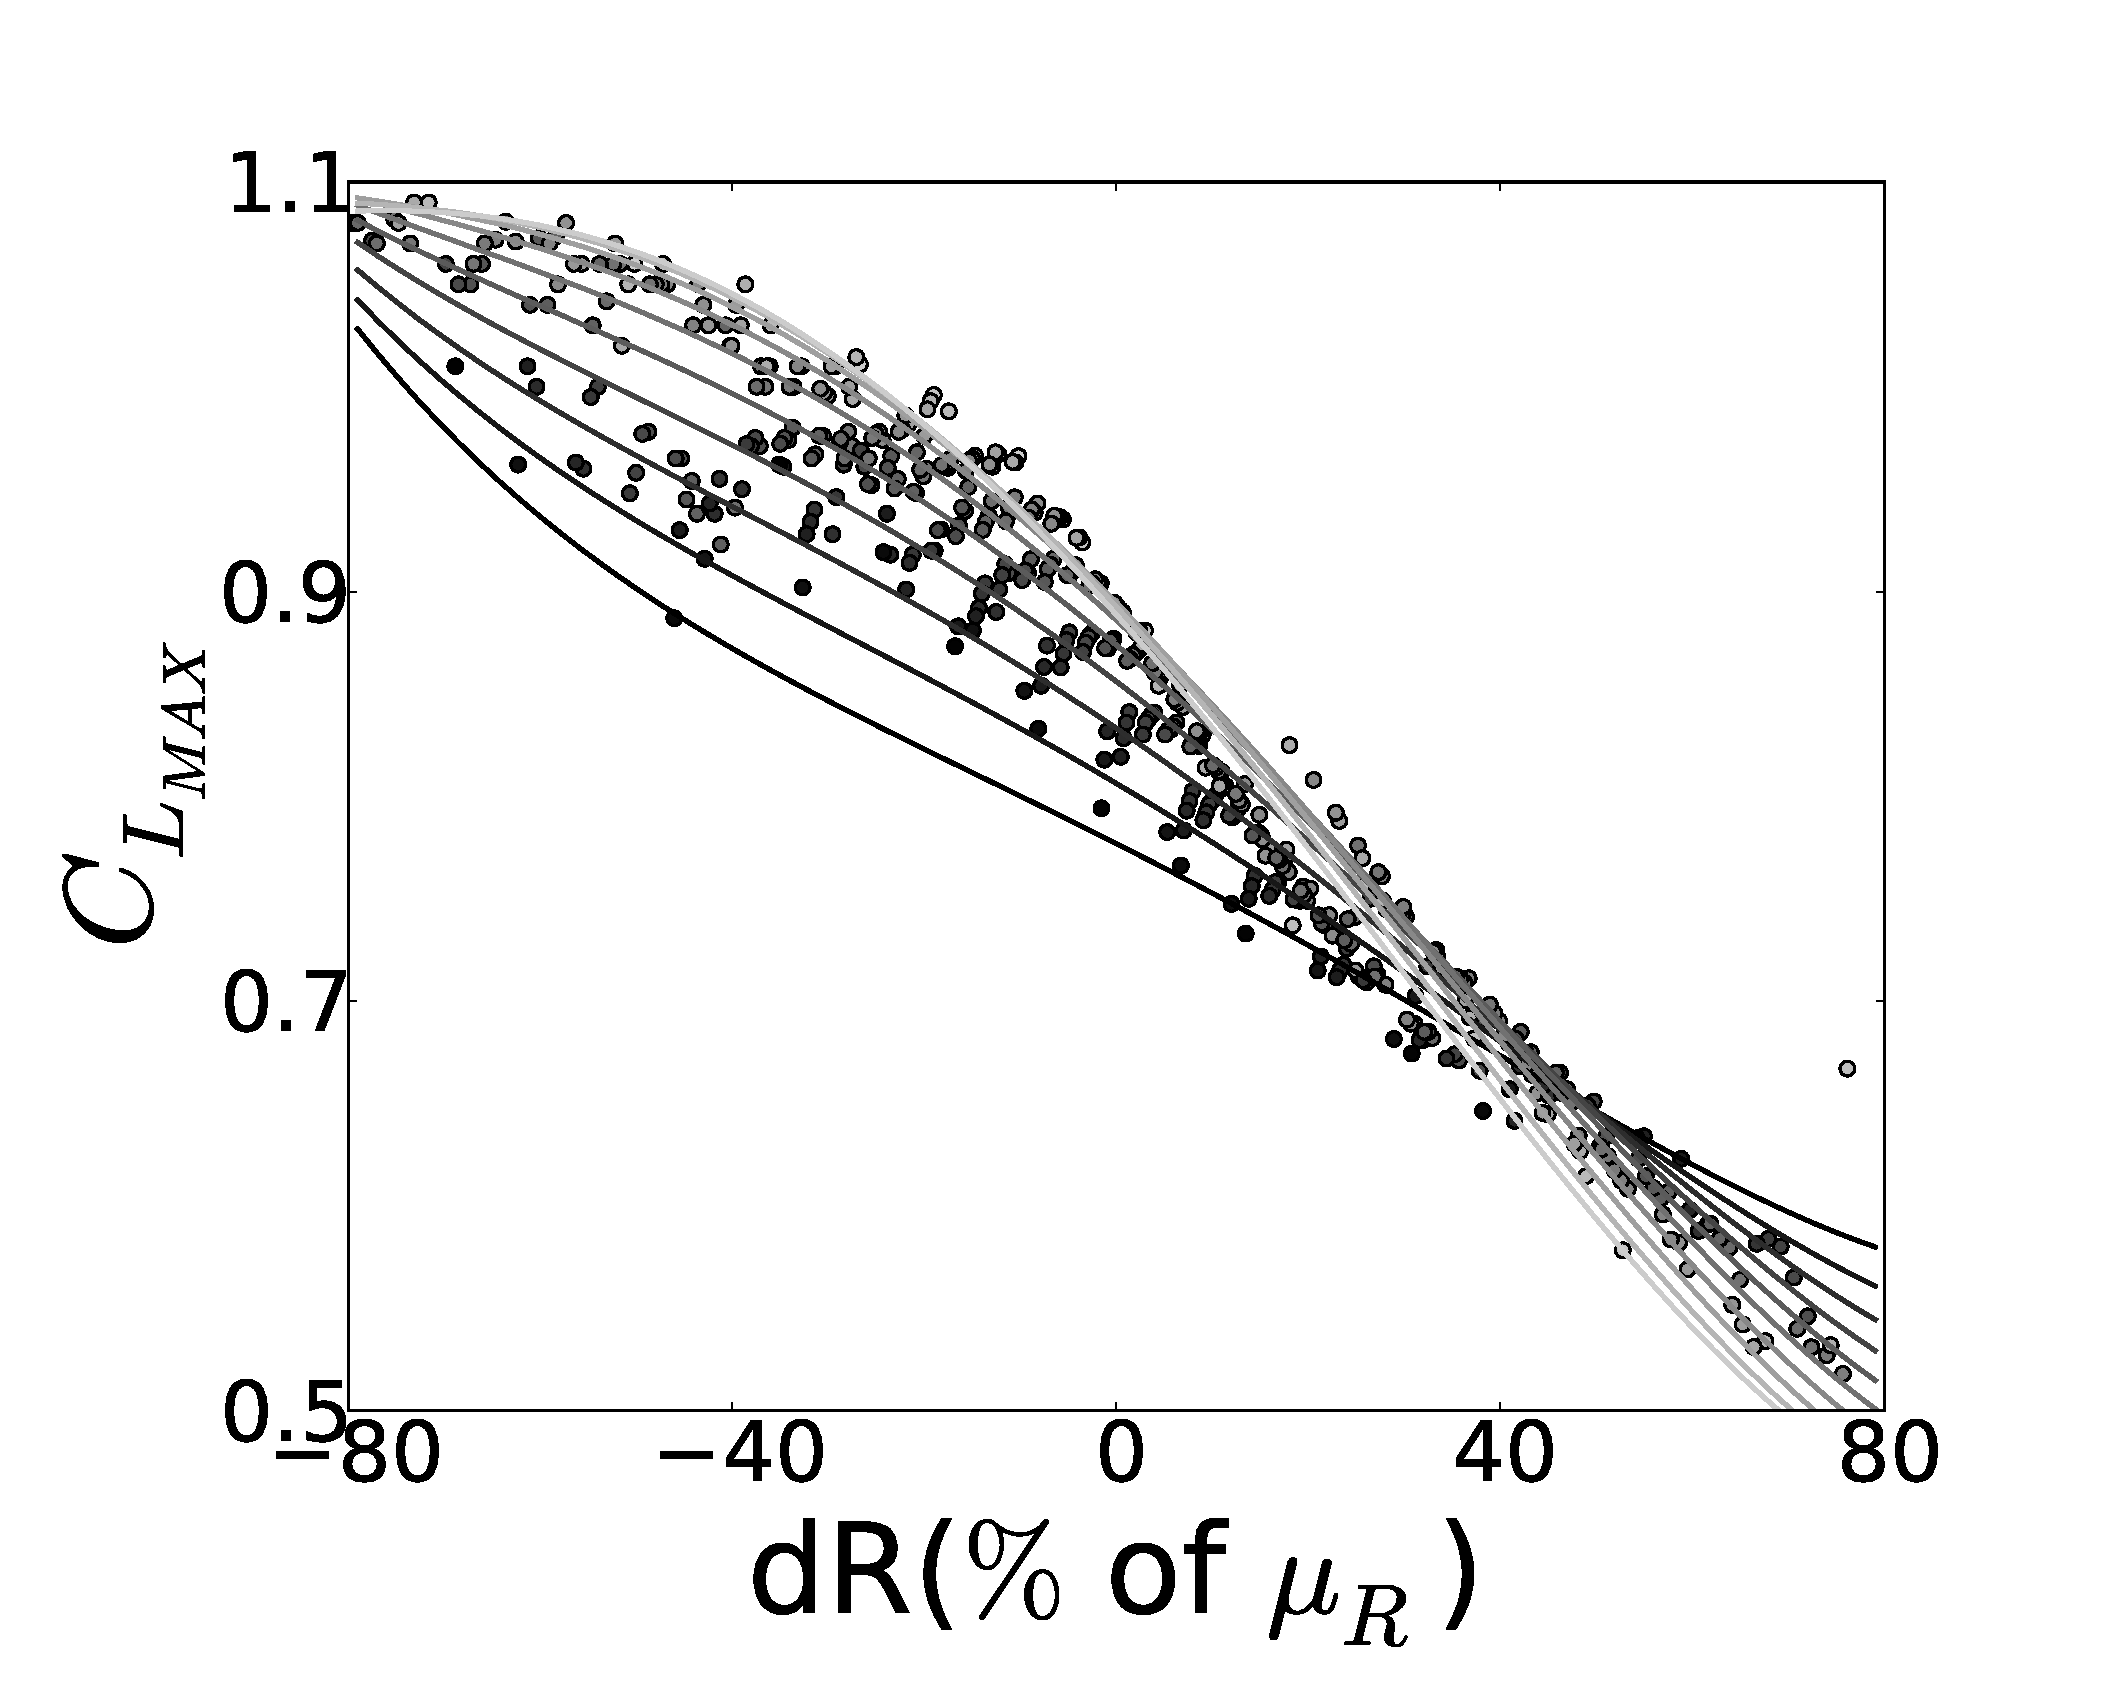
\includegraphics[width=0.65\textwidth]{MC_surrogate_LargeUnc_CL}
\end{figure}
\vspace{-0.6cm}
\begin{figure}[t]
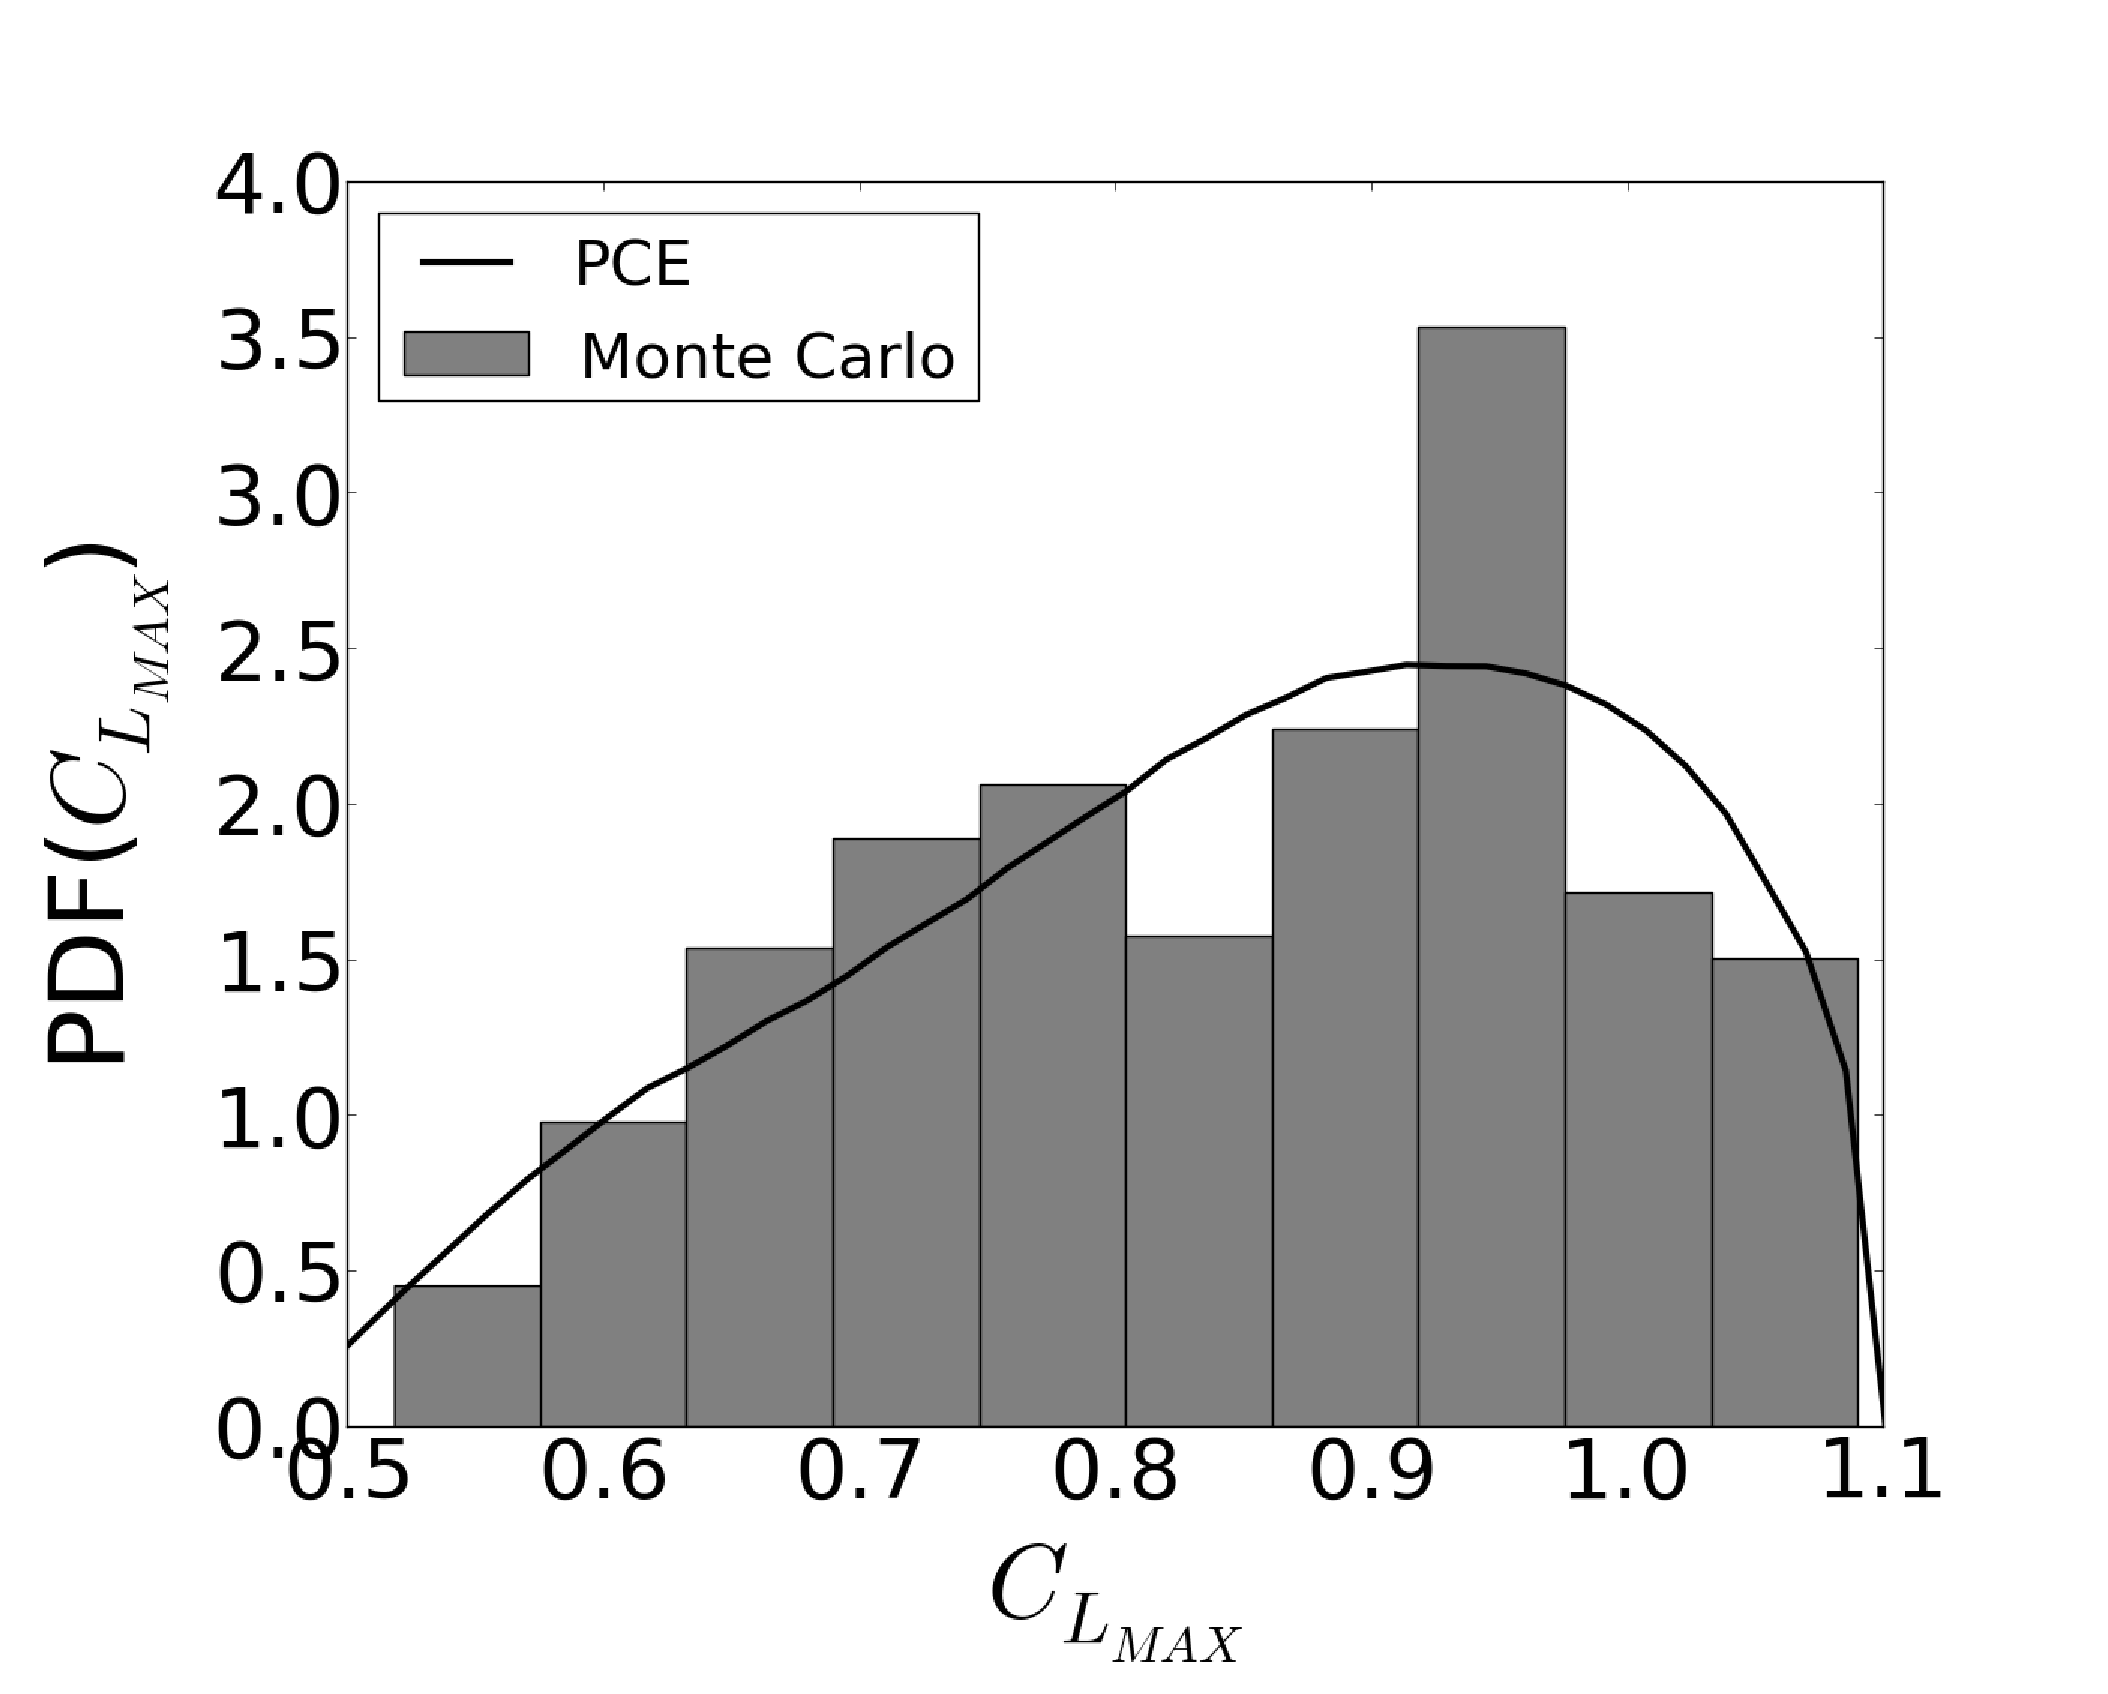
\includegraphics[width=0.65\textwidth]{MCgpcPDFLargeUnc_CL}
\caption{Lift Statistics}
\end{figure}
\end{minipage}
\begin{itemize}
\item Ridge parameters normally distributed about mean
\item Performance degrades with larger size, closer to L.E.
\end{itemize}
\end{frame}
\begin{frame}
\frametitle{Horn Study}
\label{sec-2-8}

\centering
\vspace{-0.5cm}
\begin{minipage}[t]{0.45\linewidth}
\begin{figure}[t]
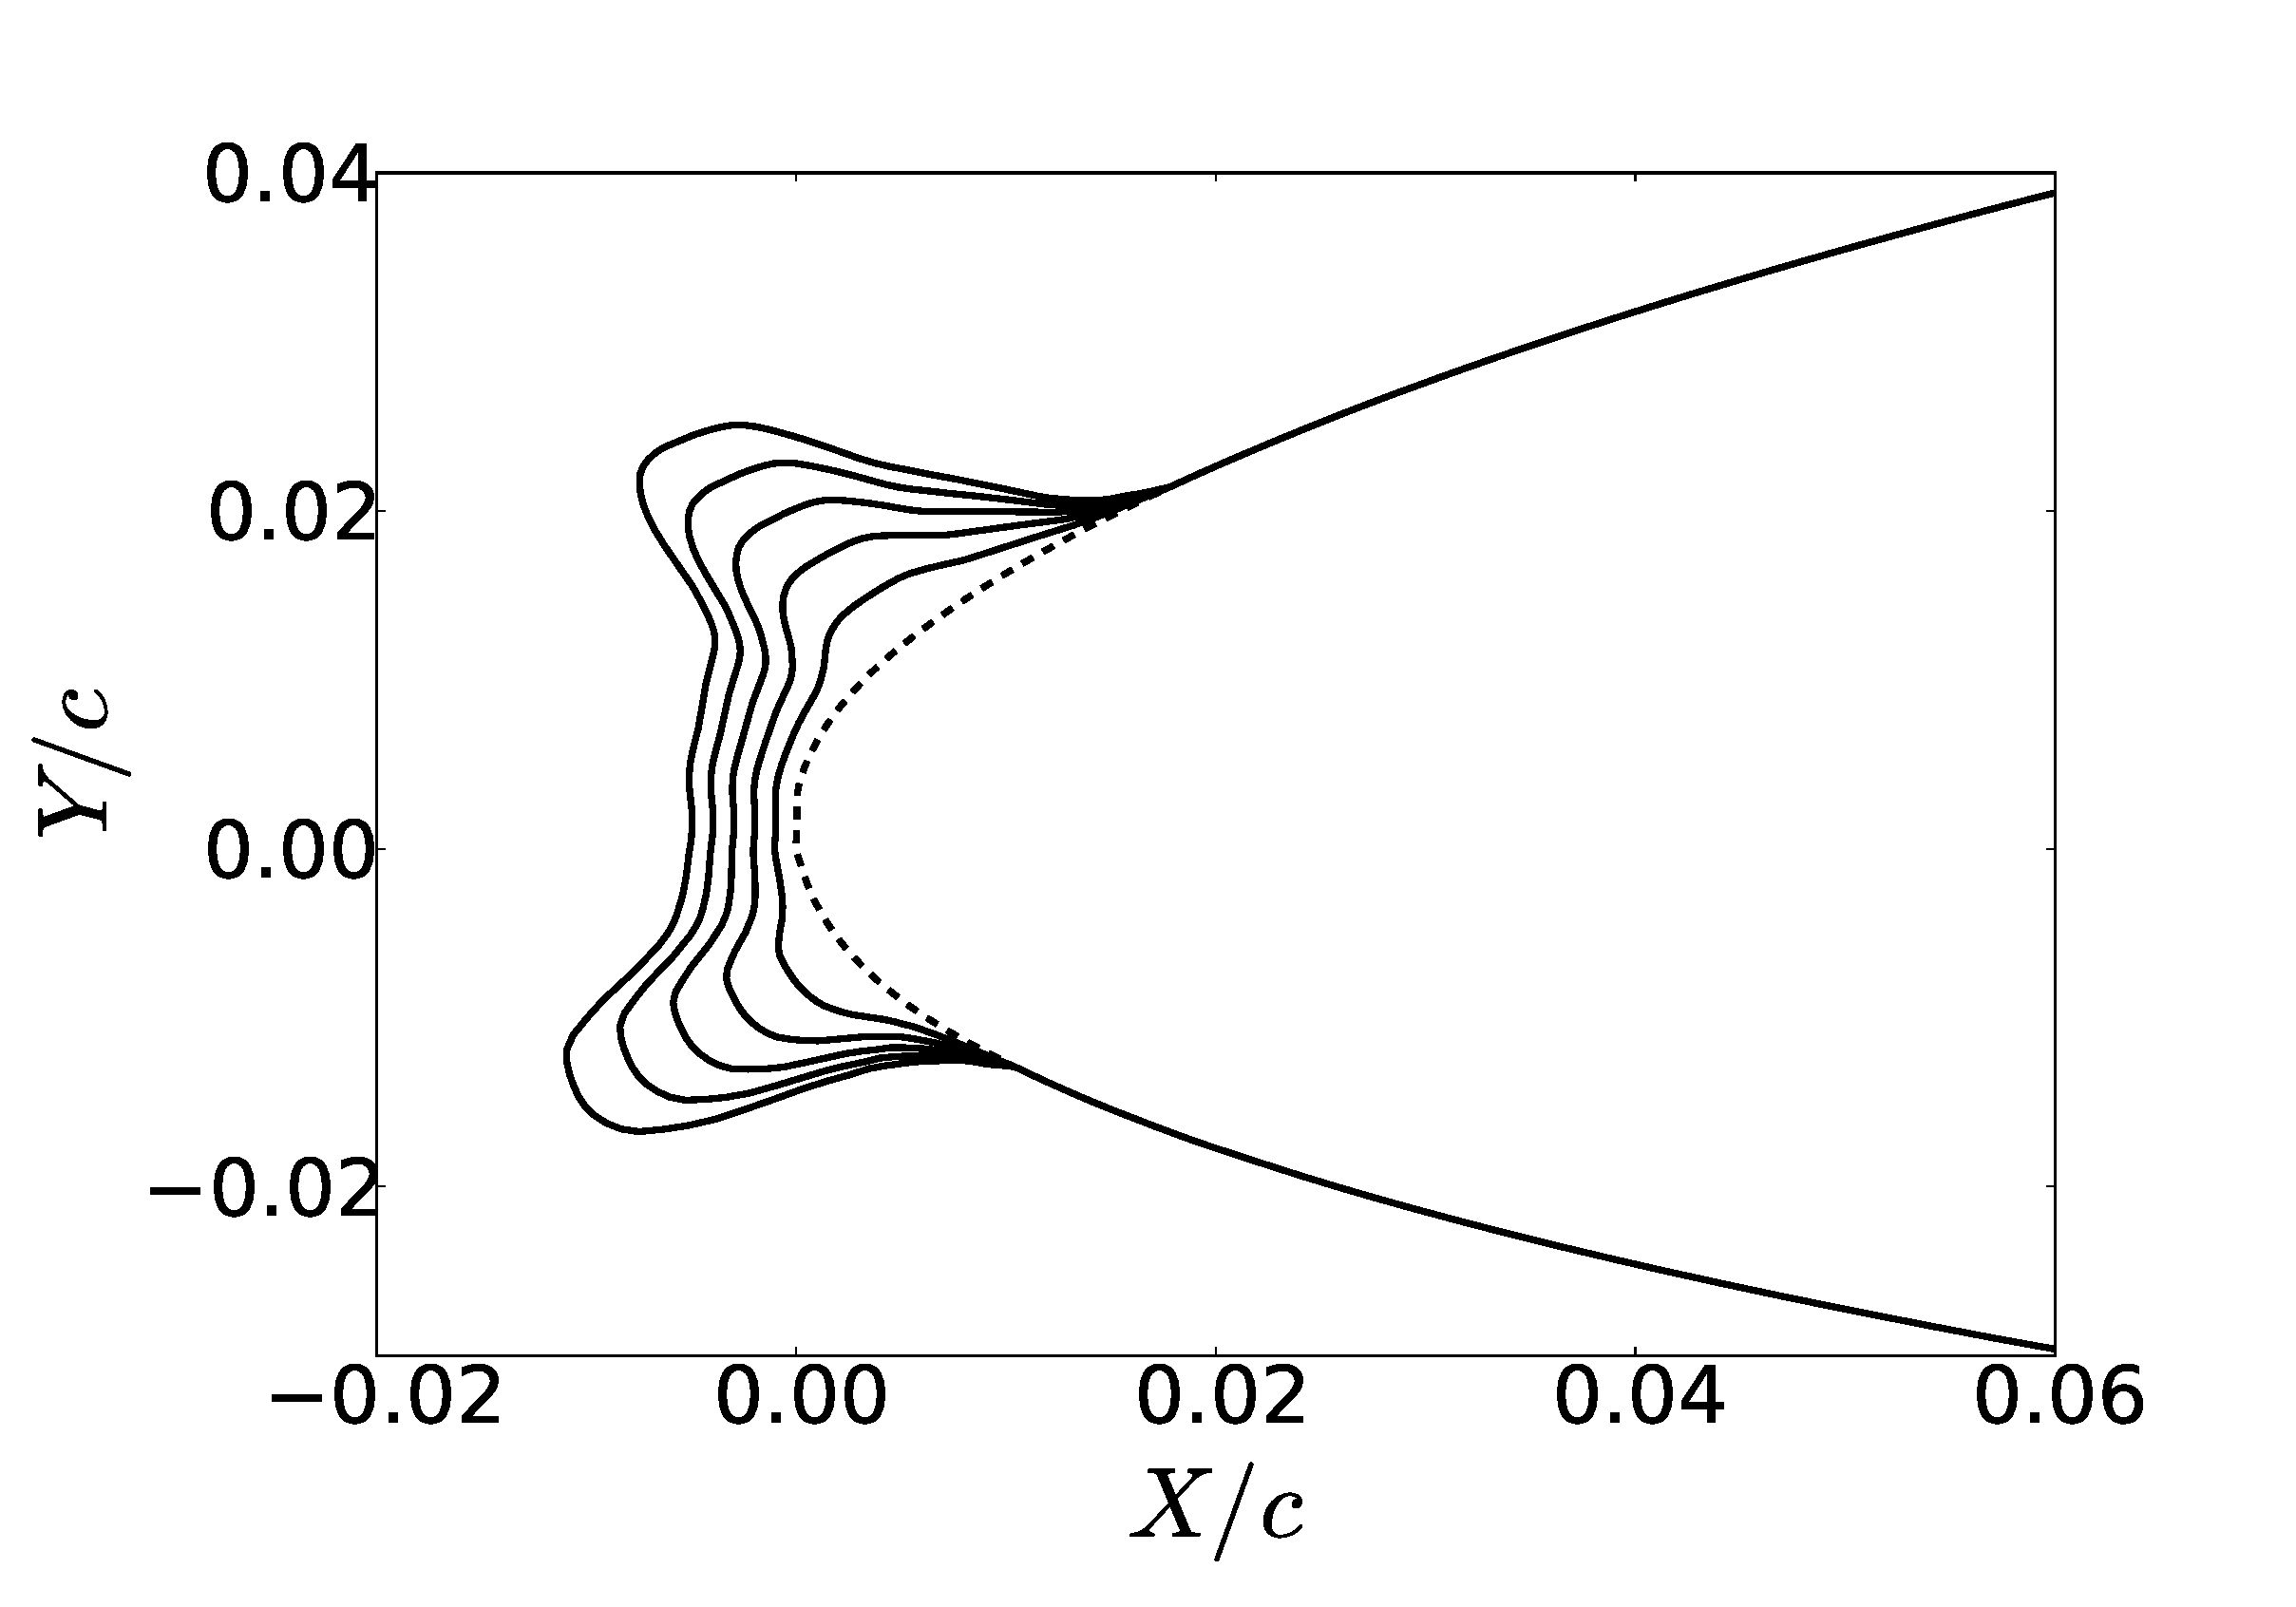
\includegraphics[width=0.75\textwidth]{HornHVariation}
\end{figure}
\vspace{-0.5cm}
\begin{figure}[t]
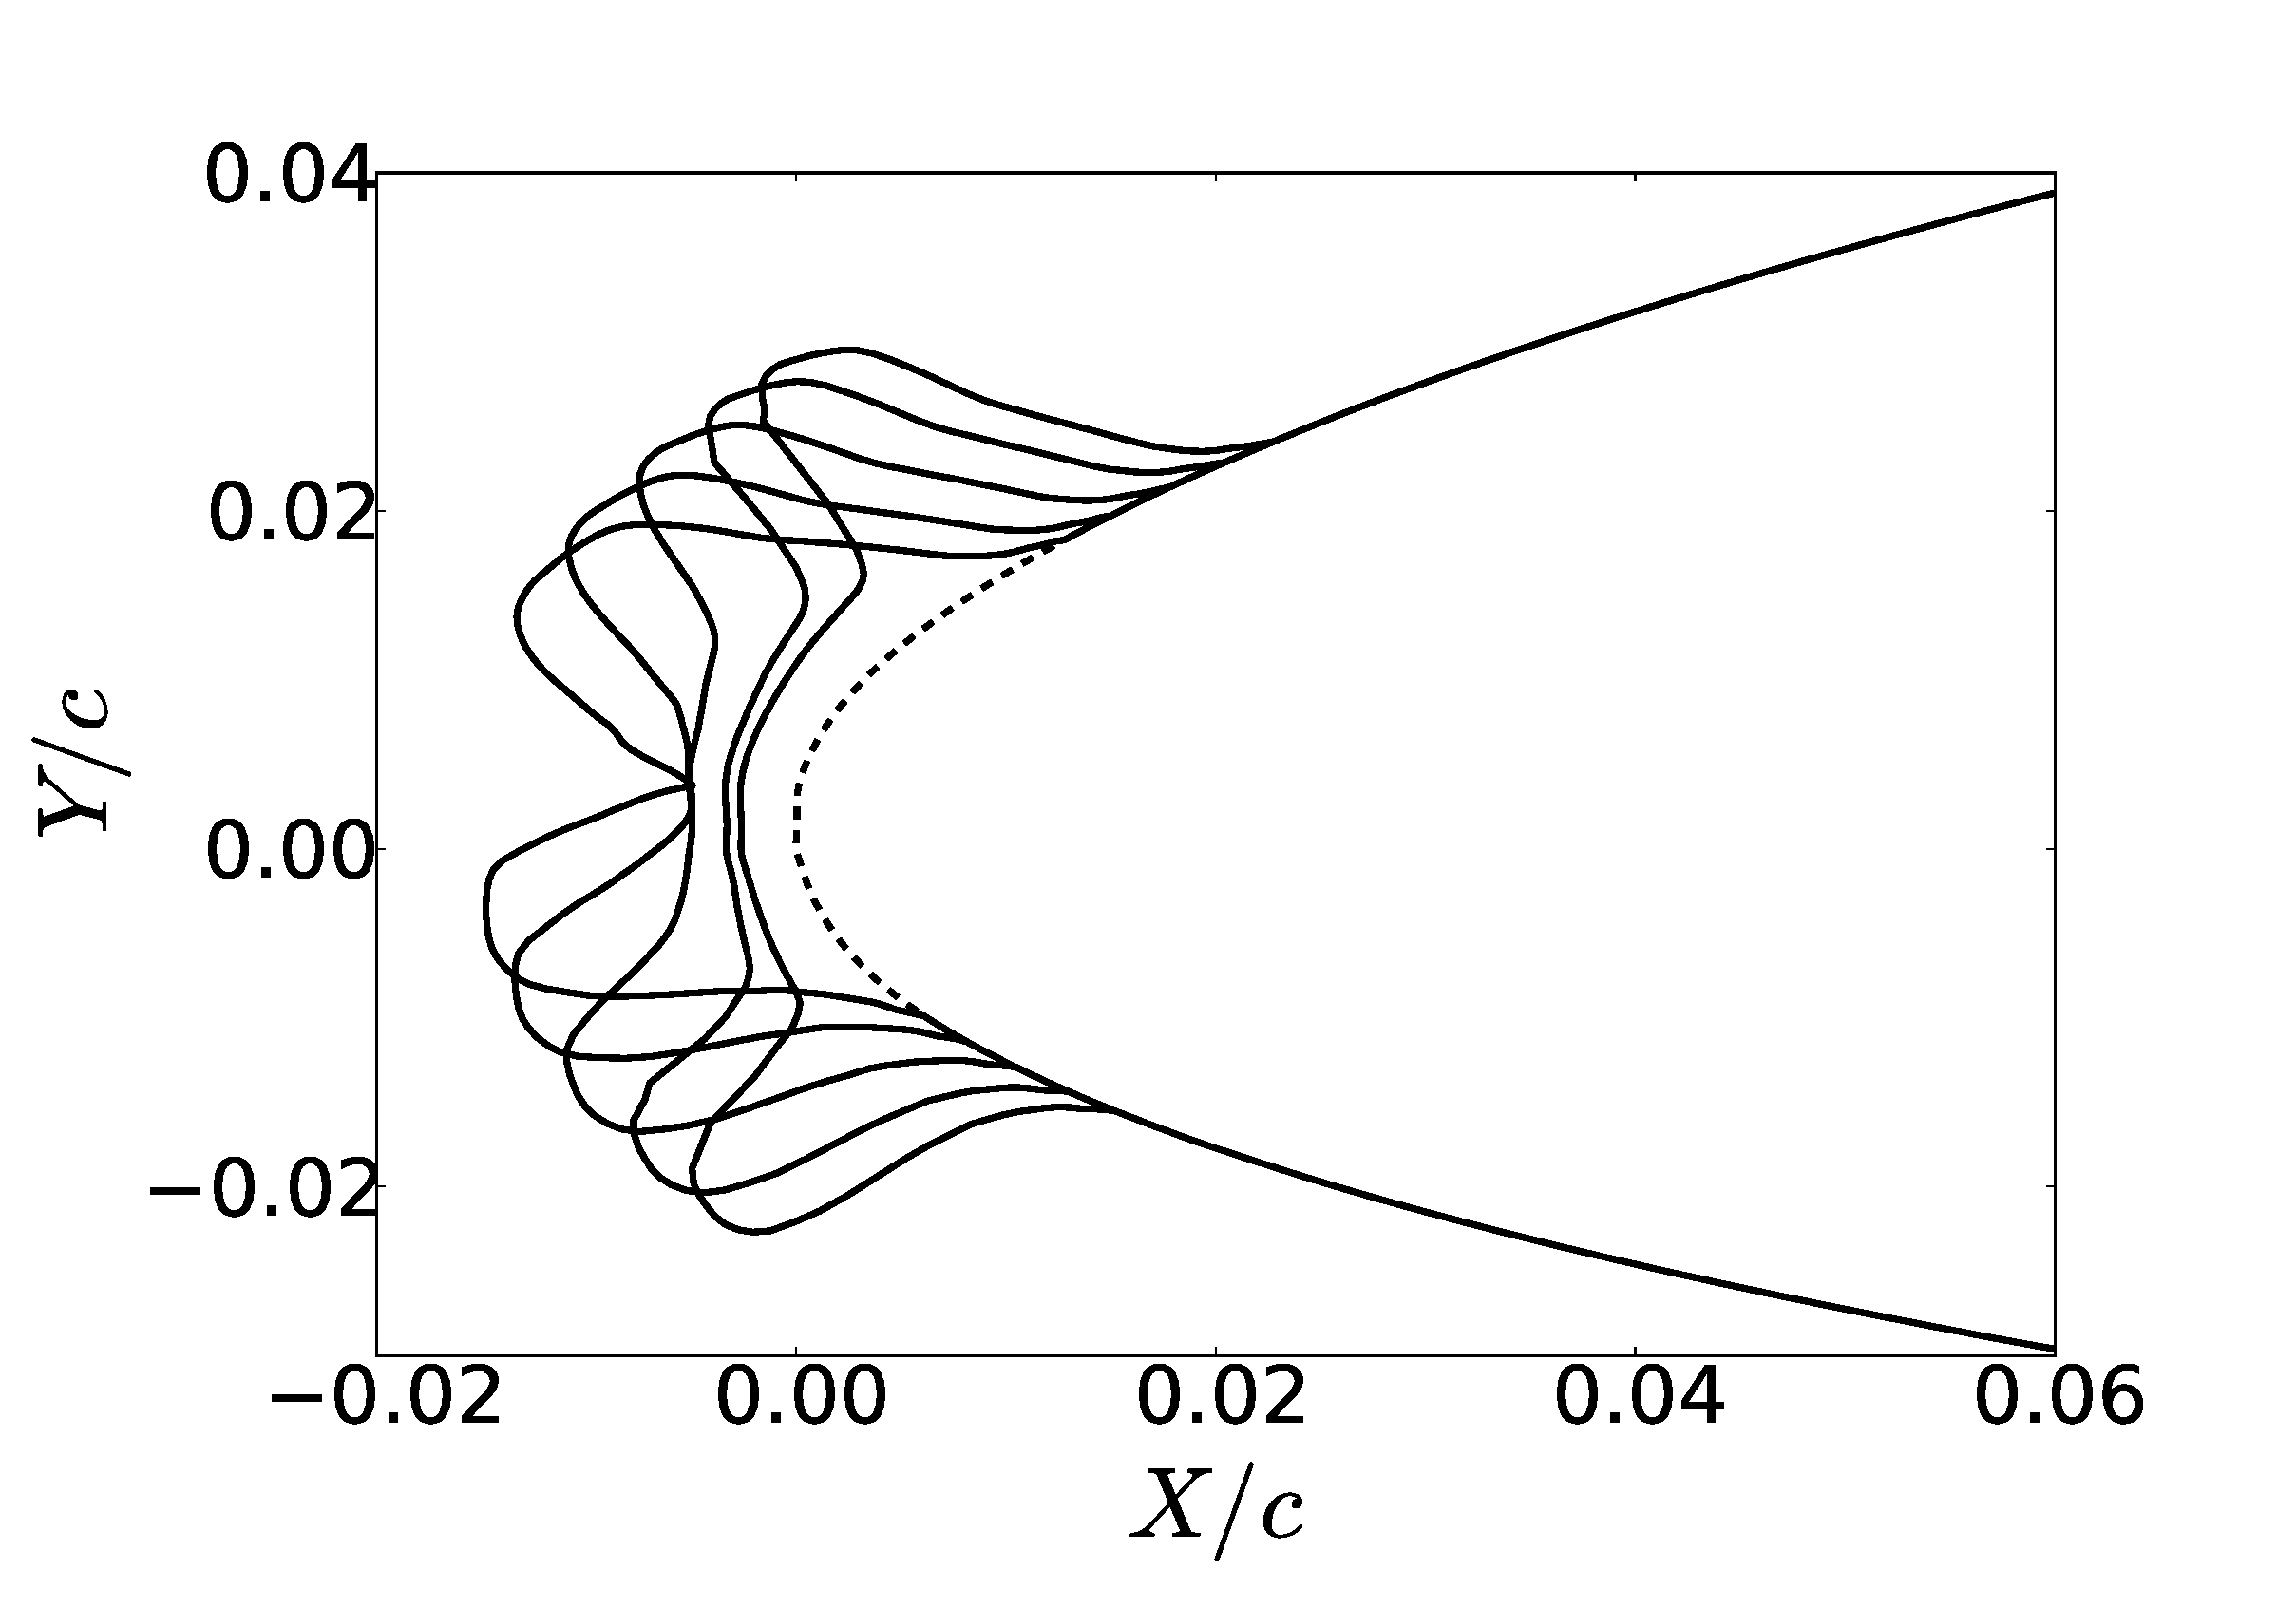
\includegraphics[width=0.75\textwidth]{HornSVariation}
\caption{Ridge Variations}
\end{figure}
\vspace{-0.5cm}
\end{minipage}
\begin{minipage}[t]{0.45\linewidth}
\begin{figure}[t]
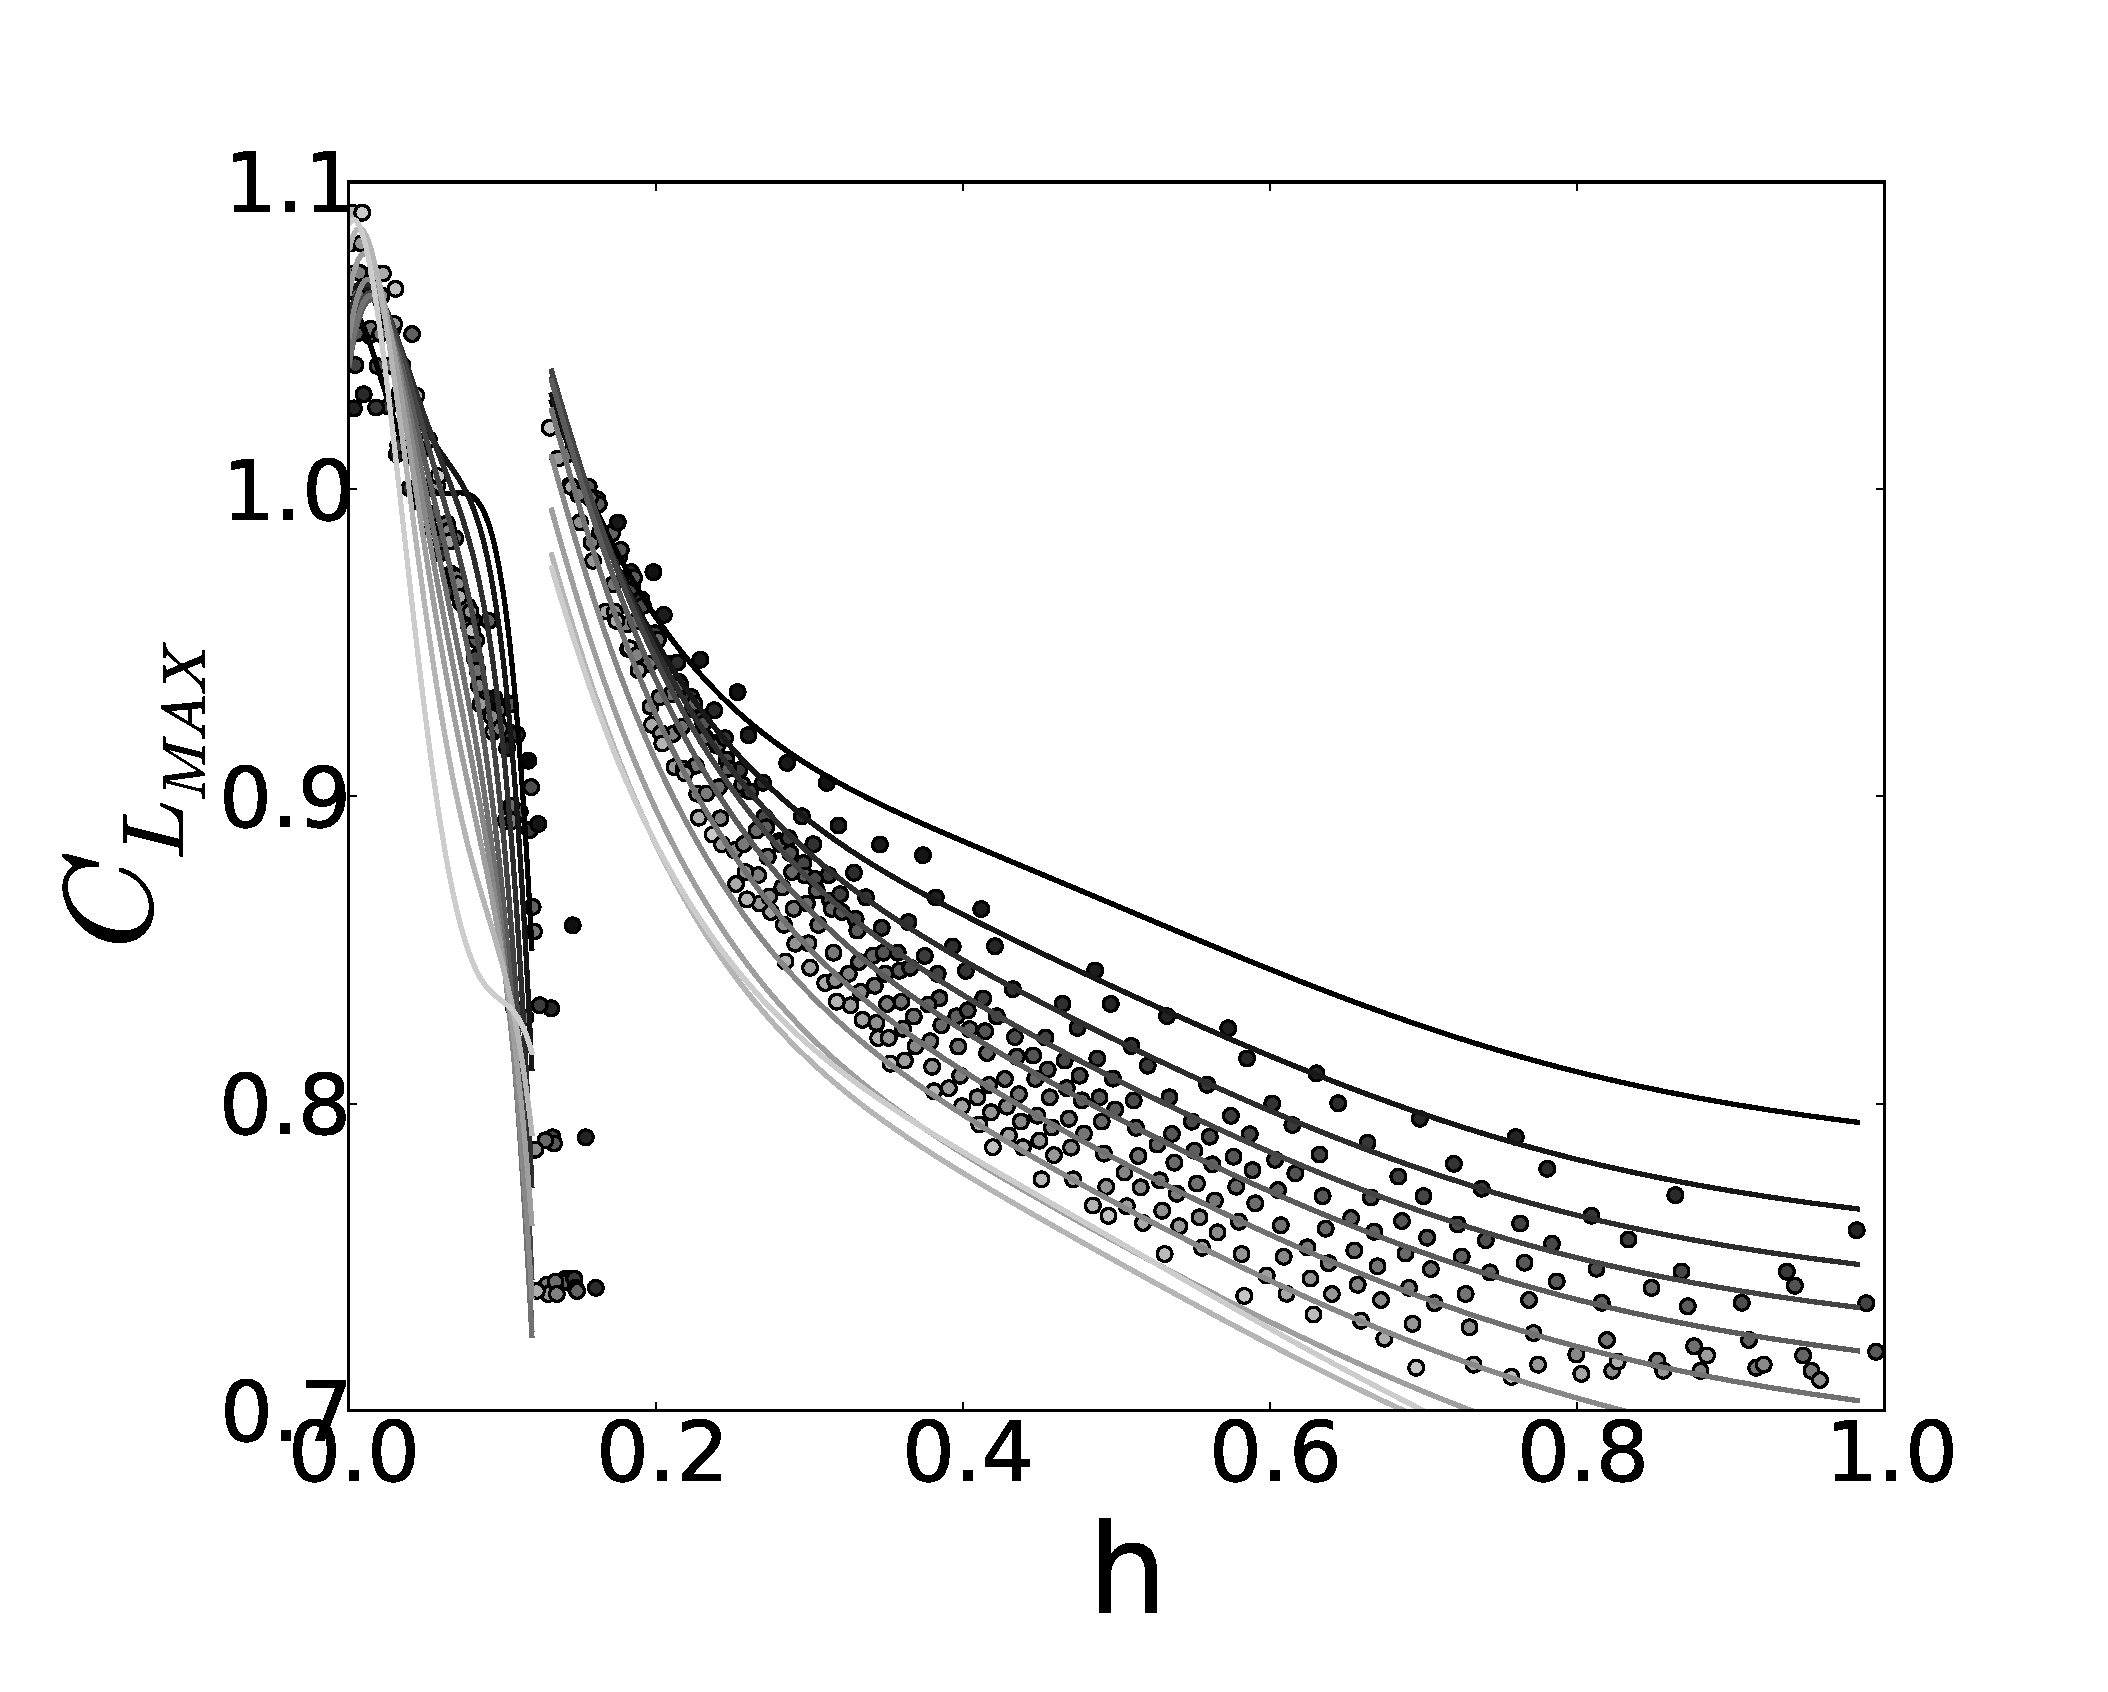
\includegraphics[width=0.65\textwidth]{CLMAX_MEGPCHORN}
\end{figure}
\vspace{-0.6cm}
\begin{figure}[t]
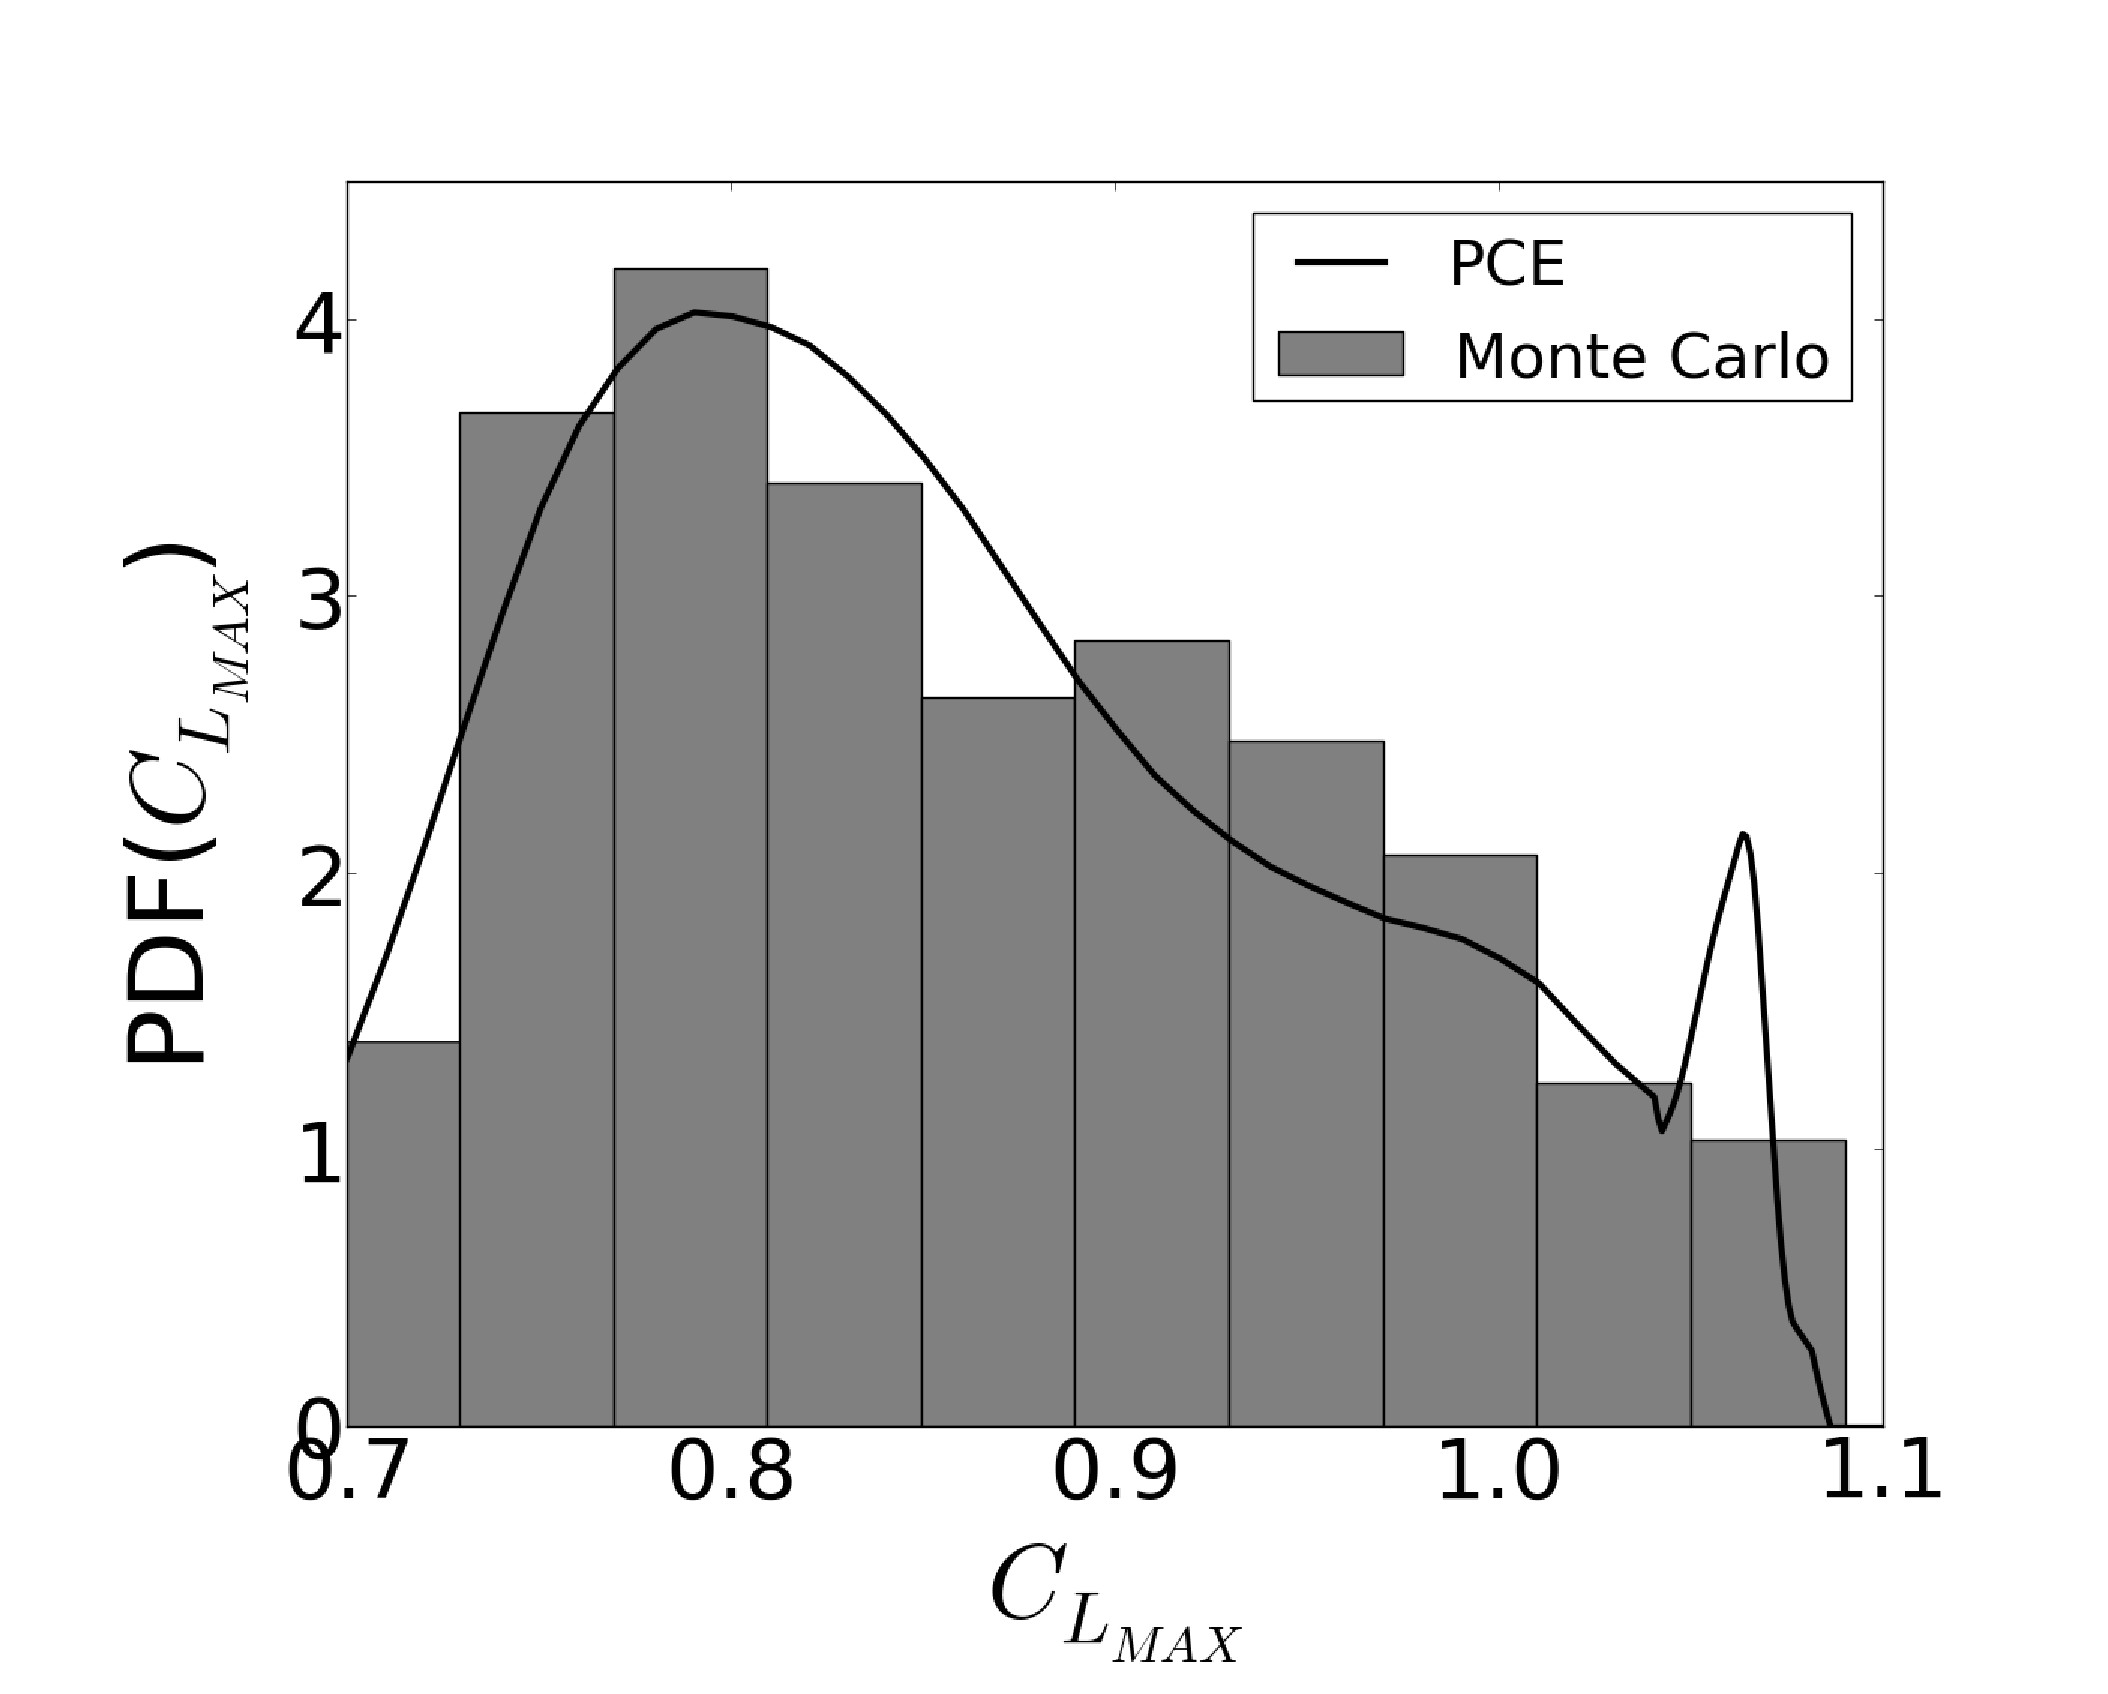
\includegraphics[width=0.65\textwidth]{MCgpcPDFMEGPCHorn_CL}
\caption{Lift Statistics}
\end{figure}
\end{minipage}
\begin{itemize}
\item Horn separation normally distributed
\item Horn height distributed as a half-Gaussian (mean = clean airfoil)
\item Performance degrades with larger horn size and separation
\end{itemize}
\end{frame}
\section{Data-Based UQ}
\label{sec-3}
\begin{frame}
\frametitle{Dataset}
\label{sec-3-1}

\vspace*{-0.0cm}\begin{figure}
      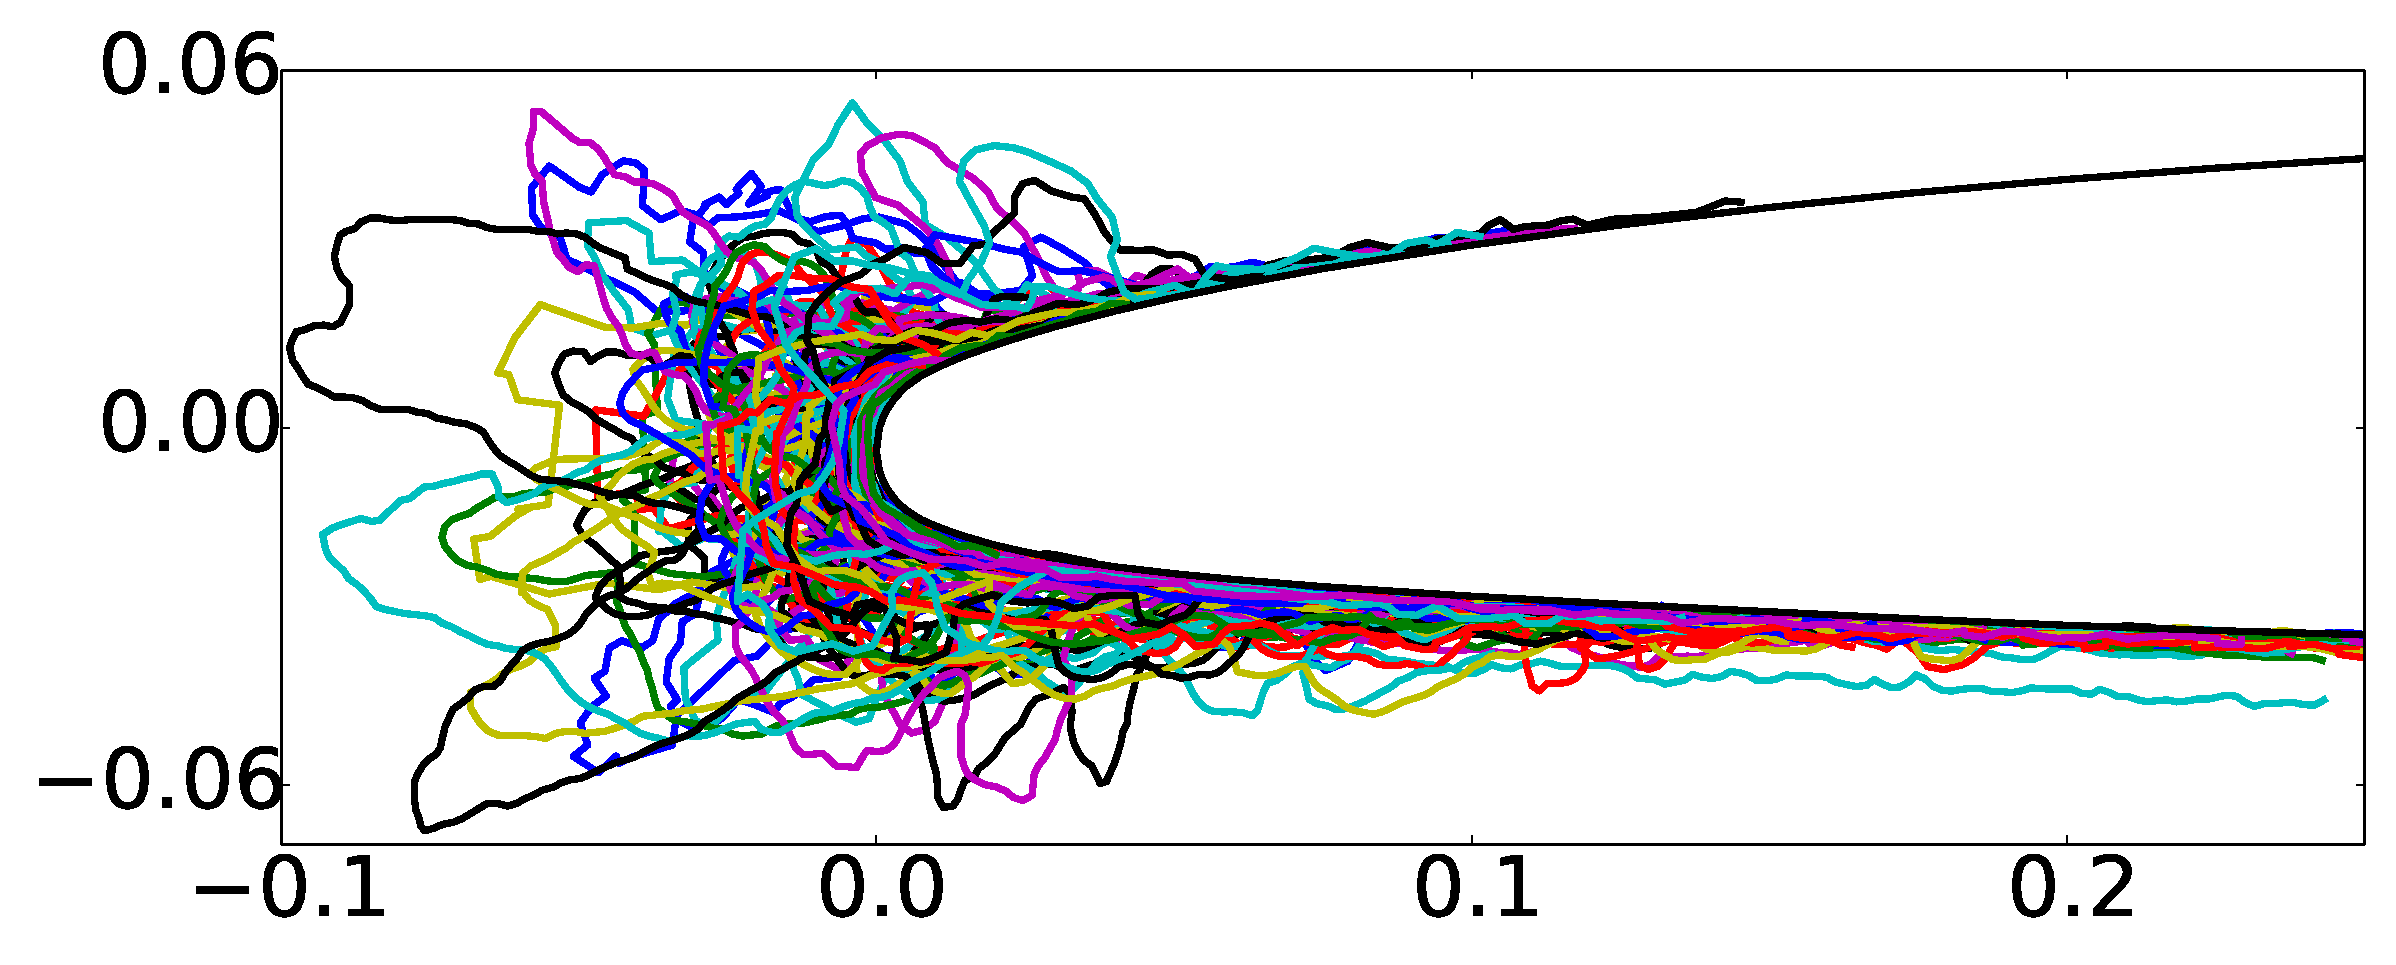
\includegraphics[width=0.5\textwidth]{GlobalDataSet}
      \caption{Wind tunnel experimental ice shapes}
\end{figure}
\begin{itemize}
\item Dataset consists of 145 experimental ice shapes
\item Obtained in icing wind tunnel at NASA Glenn\footnotemark[1]
\item Representative of a wide variety of icing conditions (temperature,
  LWC, accretion time, etc.)
\end{itemize}
\end{frame}
\begin{frame}
\frametitle{Dataset}
\label{sec-3-2}

\vspace*{-0.0cm}\begin{figure}
      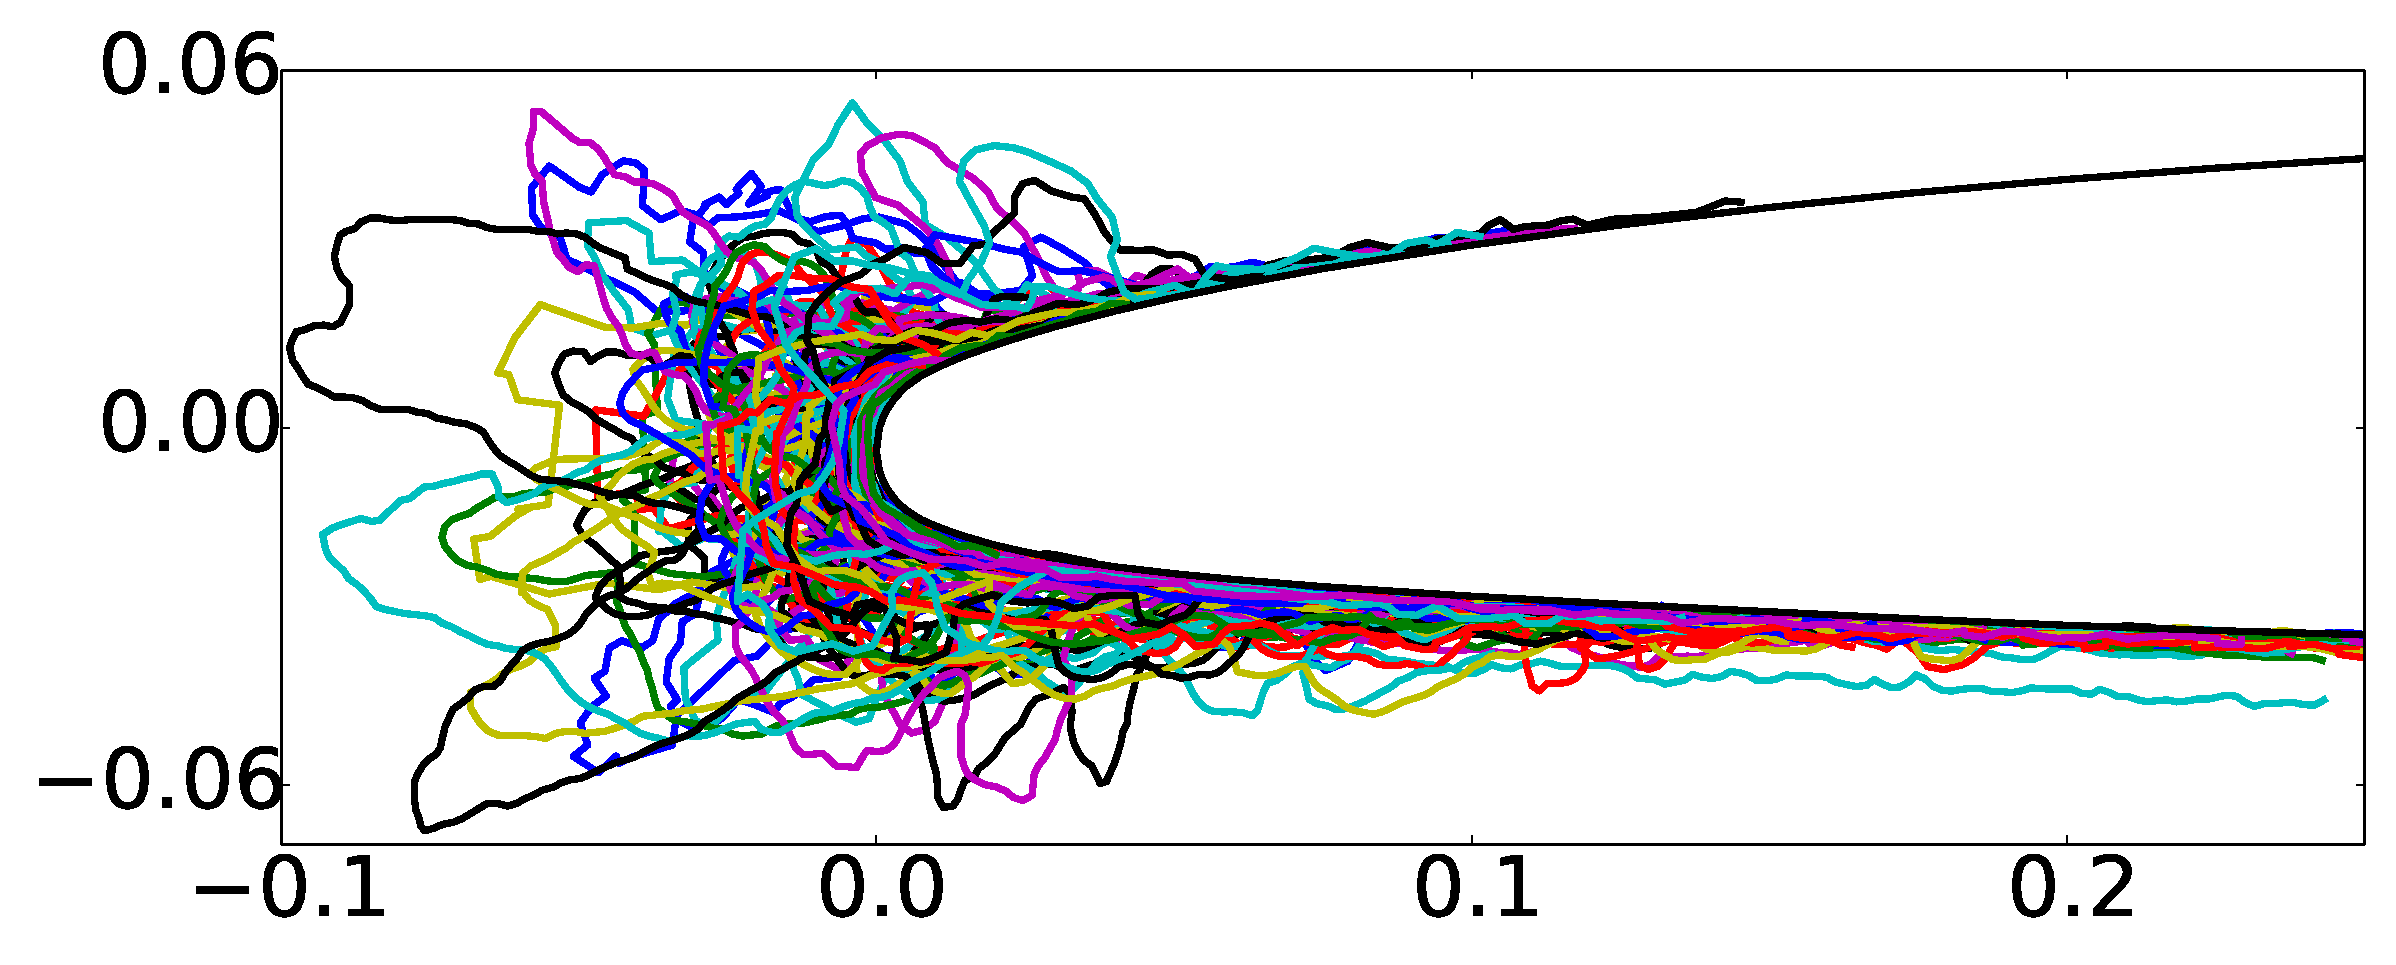
\includegraphics[width=0.5\textwidth]{GlobalDataSet}
      \caption{Wind tunnel experimental ice shapes}
\end{figure}
\textbf{Goals:}
\begin{itemize}
\item Separate shapes into self-similar groups
\item Develop low-dimensional set of shape parameters for a group
\item Perform parametric UQ on resulting parameter space
\end{itemize}
\end{frame}
\begin{frame}
\frametitle{Distance/Similarity Metric}
\label{sec-3-3}

\vspace*{-0.0cm}\begin{figure}
      \subfigure[XOR Illustration]{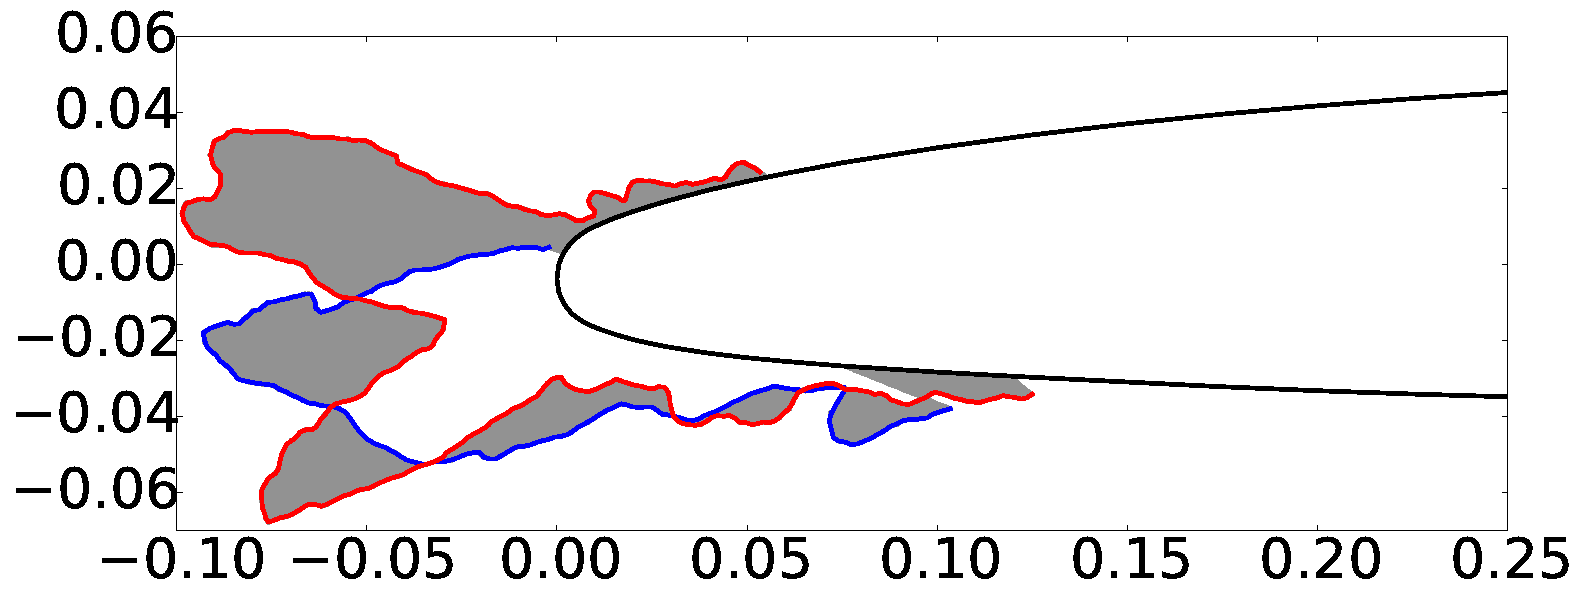
\includegraphics[width=0.4\textwidth]{XORexample.png}}
      \subfigure[Dataset Distances]{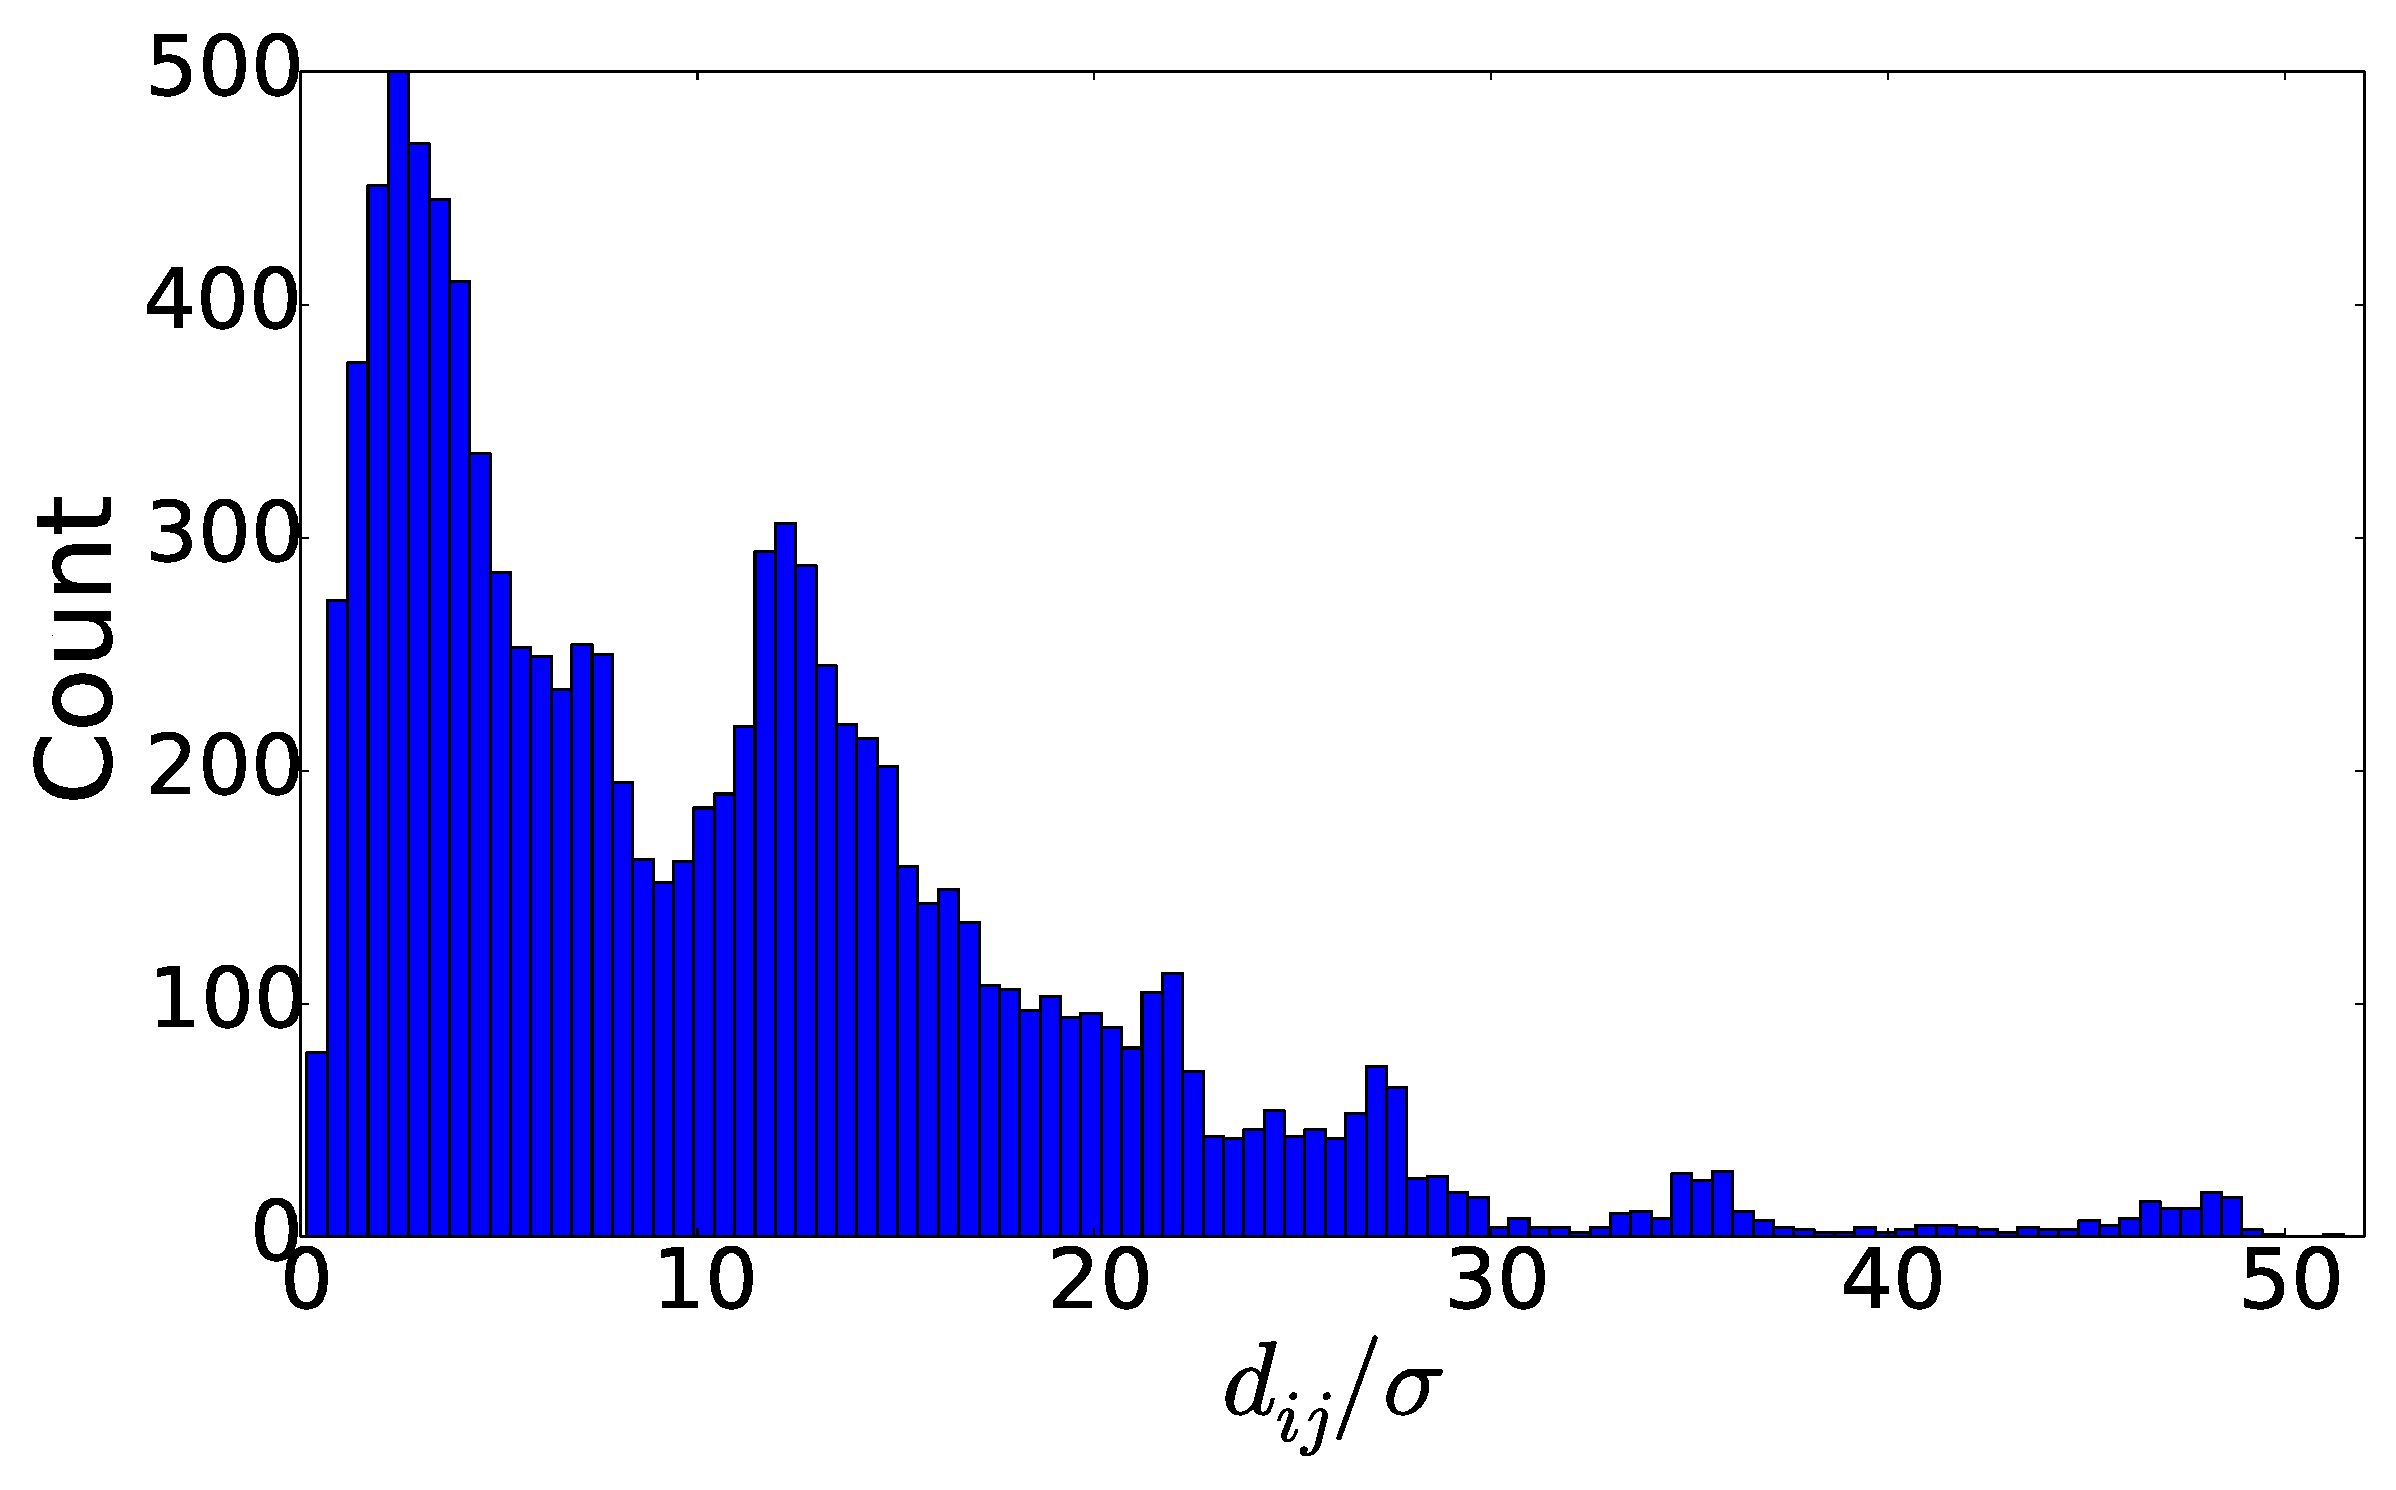
\includegraphics[width=0.4\textwidth]{XORdistances}}
      \caption{XOR distance metric}
\end{figure}
\begin{itemize}
\item Overlay dataset with a 2D Cartesian grid
\item Assign value of 1 to gridpoint if it is on the ice, 0 otherwise
\item Pick $\sigma$ based on observed peaks in data distances
\item Truncate $w_{ij}$ after $d_{ij} > 3\sigma$
\end{itemize}
\begin{equation*}
w_{ij} = \text{exp} \left(-\frac{1}{2} \frac{d_{ij}^2}{\sigma^2} \right) \;\;\;\;\;\; w_{ij} = \sum_k^{N_G} \left [ \text{XOR}(x_i,x_j) \right ]_k
\end{equation}
 
\end{frame}
\begin{frame}
\frametitle{Spectral Graph Partitioning}
\label{sec-3-4}

\textbf{Goal:} cluster shapes based upon similarity metric \\
\textbf{Methodology:} view database as an undirected graph
$\mathcal{G}(\mathcal{V},\mathcal{E})$
\begin{itemize}
\item Vertices $\mathcal{V}$ are ice shapes
\item Edges $\mathcal{E}$ are similarities between ice shapes
\item Find ``best'' partition of $\mathcal{G}(\mathcal{V},\mathcal{E})$ into subsets A and B
\end{itemize}
\vspace*{-1.25cm}
\begin{figure}
   \includegraphics[width=0.5\textwidth]{GraphPartition.png}
   \vspace{-2.25cm}
   \caption{Graph partition illustration} 
\end{figure}
\end{frame}
\begin{frame}
\frametitle{Spectral Graph Partitioning}
\label{sec-3-5}

\textbf{Approach:}\footnote{Shi \& Malik. \emph{Normalized Cuts and Image Segmentation}, 2000.
 }
\begin{itemize}
\item Calculate graph Laplacian using similarity metric
\begin{itemize}
\item Similarity matrix: $W = w(i,j)$
\item Degree matrix: $D = \text{diag}(d_k) \;\;\; , \;\;\; d_k = \sum_{j=1}^N w(v_k,v_j) \;\;\; , \;\;\; k=1 \cdots N$
\item Laplacian matrix: $L = D - W$
\end{itemize}
\item Eigenvectors with zero eigenvalue identify disconnected subsets
\begin{itemize}
\item E.g., $L \bv{1} = \bv{0}$ <---> entire graph is disconnected
\end{itemize}
\item First nonzero eigenvector (Fiedler vector) identifies optimal
    partition of connected vertices within subsets
\begin{itemize}
\item Approximates solution of \emph{average cut} formulation: \\ 
$P(A,B) = \text{min}_{A \in \mathcal{V}} \left \lbrace \frac{\text{cut}(A,B)}{| A |} + \frac{\text{cut}(A,B)}{| B |} \right \rbrace$ \\
      $|A| = \text{Number of vertices in }A$ \\
      $\text{cut}(A,B) = \sum_{u \in A,v \in B} w(u,v)$
\item Eigenvectors close to zero similarly identify good partitions
\end{itemize}
\end{itemize}
\end{frame}
\begin{frame}
\frametitle{Spectral Graph Partitioning}
\label{sec-3-6}

\begin{figure}
    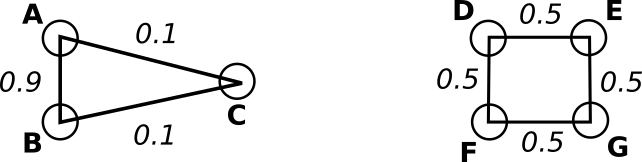
\includegraphics[width=0.5\textwidth]{ExampleGraph.png}
    \caption{Toy example}
\end{figure}
\begin{equation*}
L = \begin{bmatrix}
1  & -0.9 & -0.1 & 0 & 0 & 0 & 0 \\
-0.9 & 1  & -0.1 & 0 & 0 & 0 & 0 \\
-0.1 & -0.1 & 0.2  & 0 & 0 & 0 & 0 \\
0    & 0    & 0    & 1 & -0.5 & -0.5 & 0 \\
0    & 0    & 0    & -0.5 & 1 & 0 & -0.5 \\
0    & 0    & 0    & -0.5 & 0 & 1 & -0.5 \\
0    & 0    & 0    & 0 & -0.5 & -0.5 & 1 \\ 
\end{bmatrix}
\end{equation}
\end{frame}
\begin{frame}
\frametitle{Spectral Graph Partitioning}
\label{sec-3-7}

\vspace*{-0.0cm}\begin{figure}
      \subfigure[$\lambda_1 = 0$]{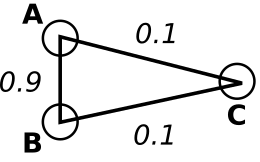
\includegraphics[width=0.15\textwidth]{ExampleGraphEvec1.png}}
      \subfigure[$\lambda_2 = 0$]{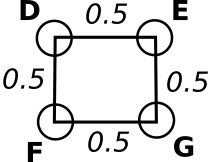
\includegraphics[width=0.15\textwidth]{ExampleGraphEvec2.png}}
      \caption{Disconnected subsets}
\end{figure}
\vspace*{-0.0cm}\begin{figure}
      \subfigure[$\lambda_3$]{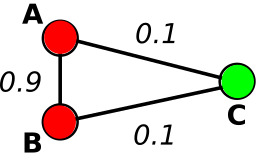
\includegraphics[width=0.15\textwidth]{ExampleGraphEvec3.png}}
      \subfigure[$\lambda_4$]{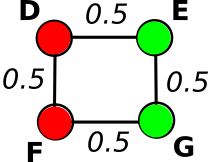
\includegraphics[width=0.15\textwidth]{ExampleGraphEvec4.png}}
      \subfigure[$\lambda_5$]{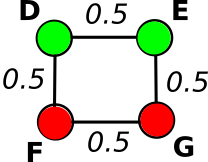
\includegraphics[width=0.15\textwidth]{ExampleGraphEvec5.png}}
      \caption{Clustering within subsets}
\end{figure}
\begin{itemize}
\item Two zero eigenvalues, corresponding to two clusters
\item Eigenvalues close to zero give good partitions within clusters
\end{itemize}
\end{frame}
\begin{frame}
\frametitle{Graph Laplacian}
\label{sec-3-8}

\vspace*{-0.0cm}\begin{figure}
      \subfigure[Similarity Matrix]{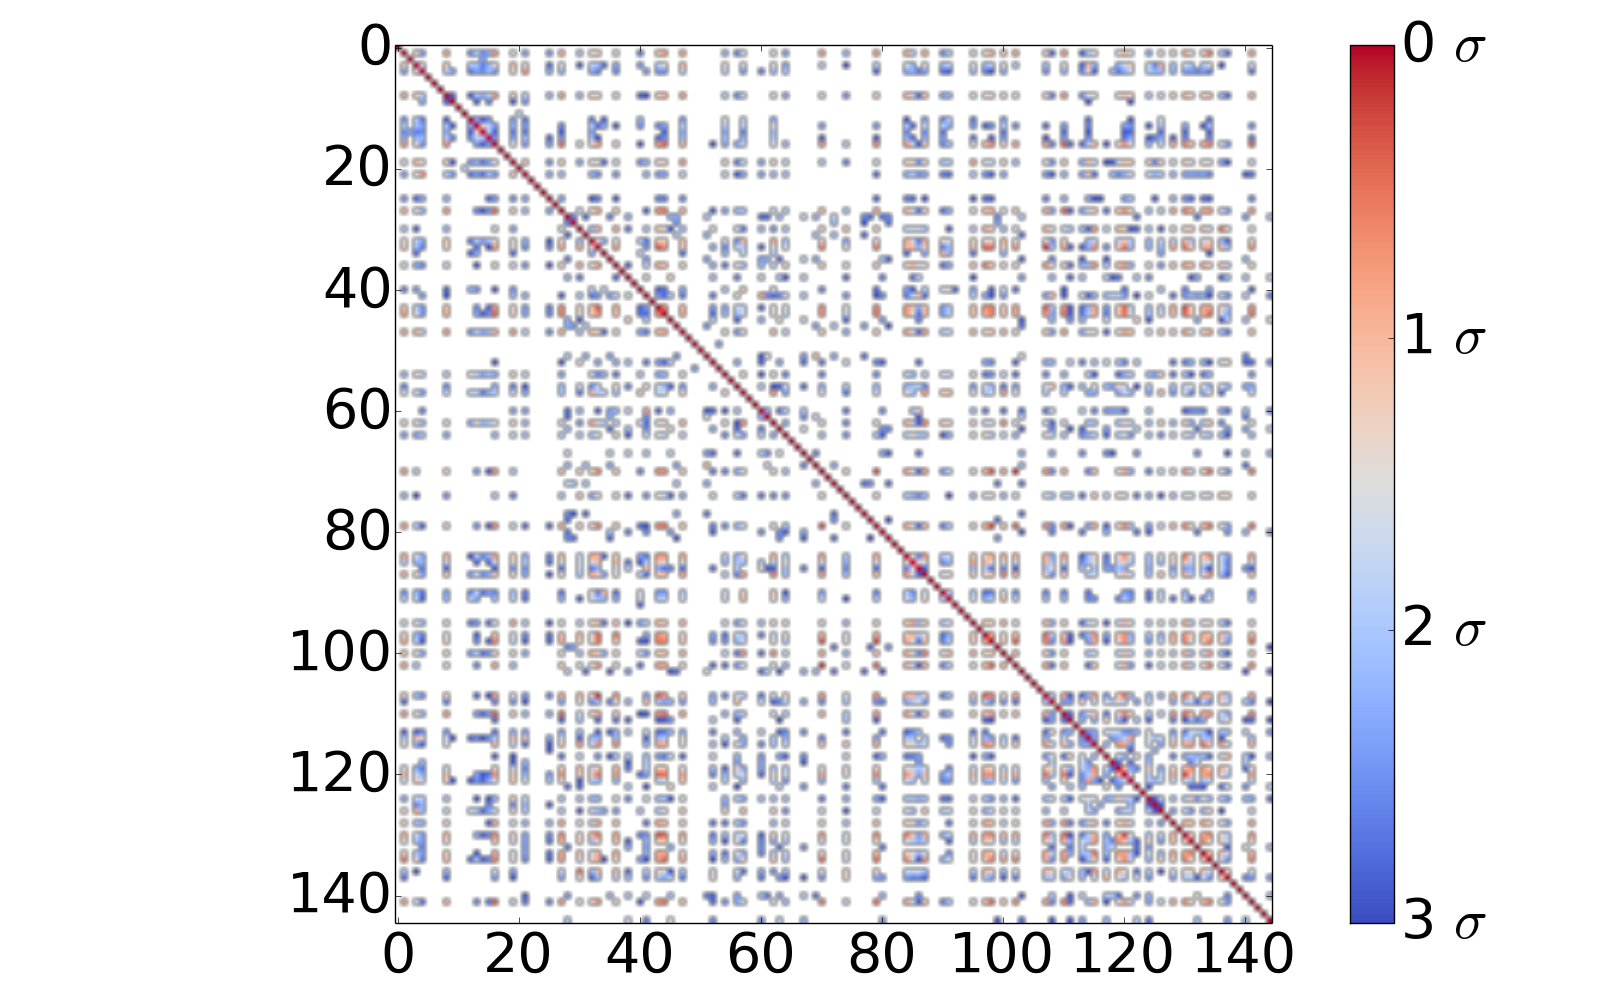
\includegraphics[width=0.4\textwidth]{DistanceMatrixUnordered.png}}
      \subfigure[Eigenvalue Magnitudes]{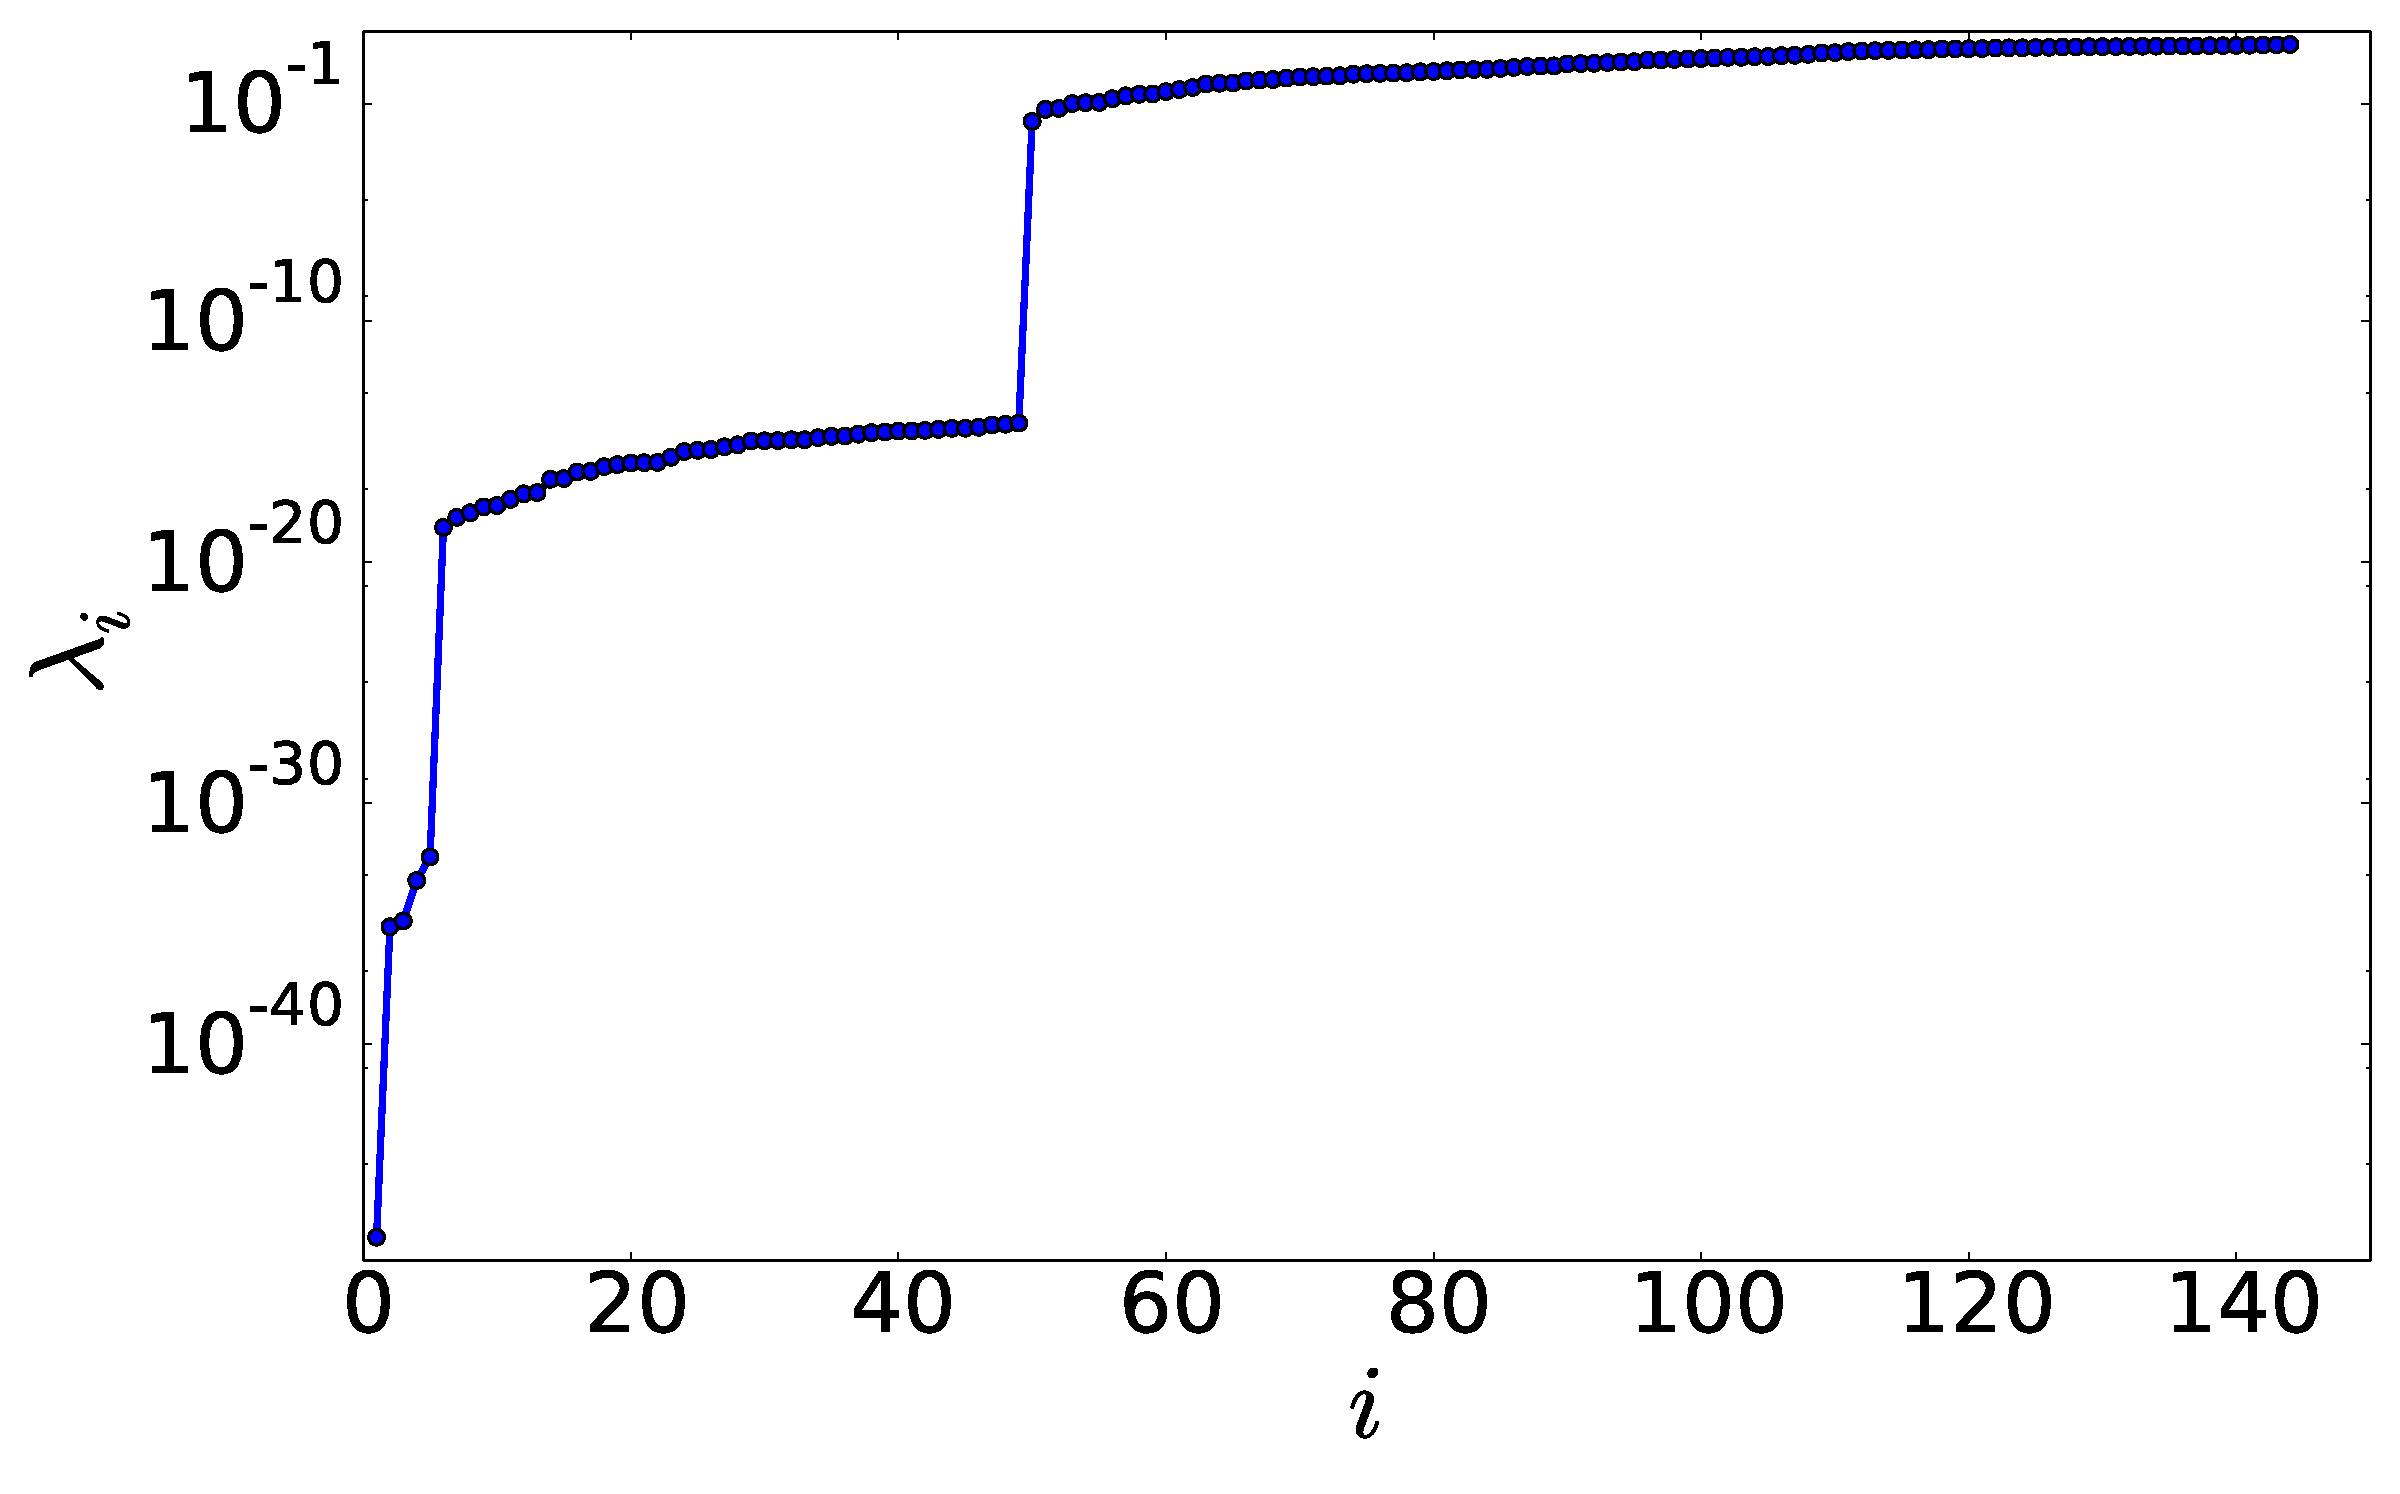
\includegraphics[width=0.4\textwidth]{LaplacianEvals}}
      \caption{Laplacian visualization and eigenvalues}
\end{figure}
\begin{itemize}
\item Many zero eigenvalues because many of the dataset elements are
  completely unconnected from each other
\end{itemize}
\end{frame}
\begin{frame}
\frametitle{Clusters}
\label{sec-3-9}

\vspace*{-0.0cm}\begin{figure}
      \subfigure[Similarity Matrix]{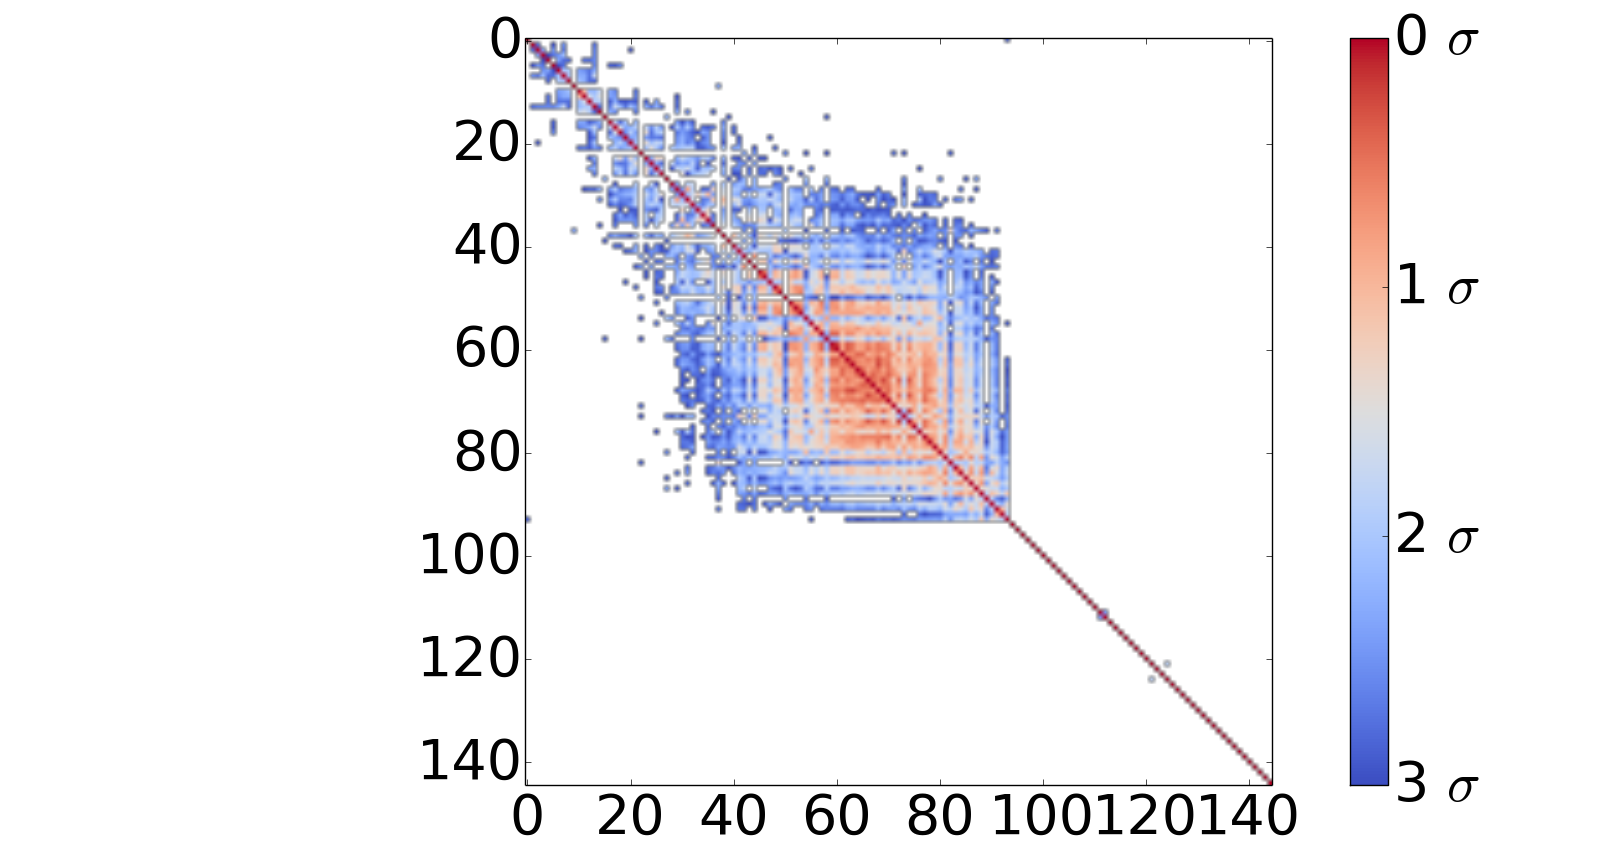
\includegraphics[width=0.45\textwidth]{DistanceMatrixOrdered.png}}
      \subfigure[Ice shapes]{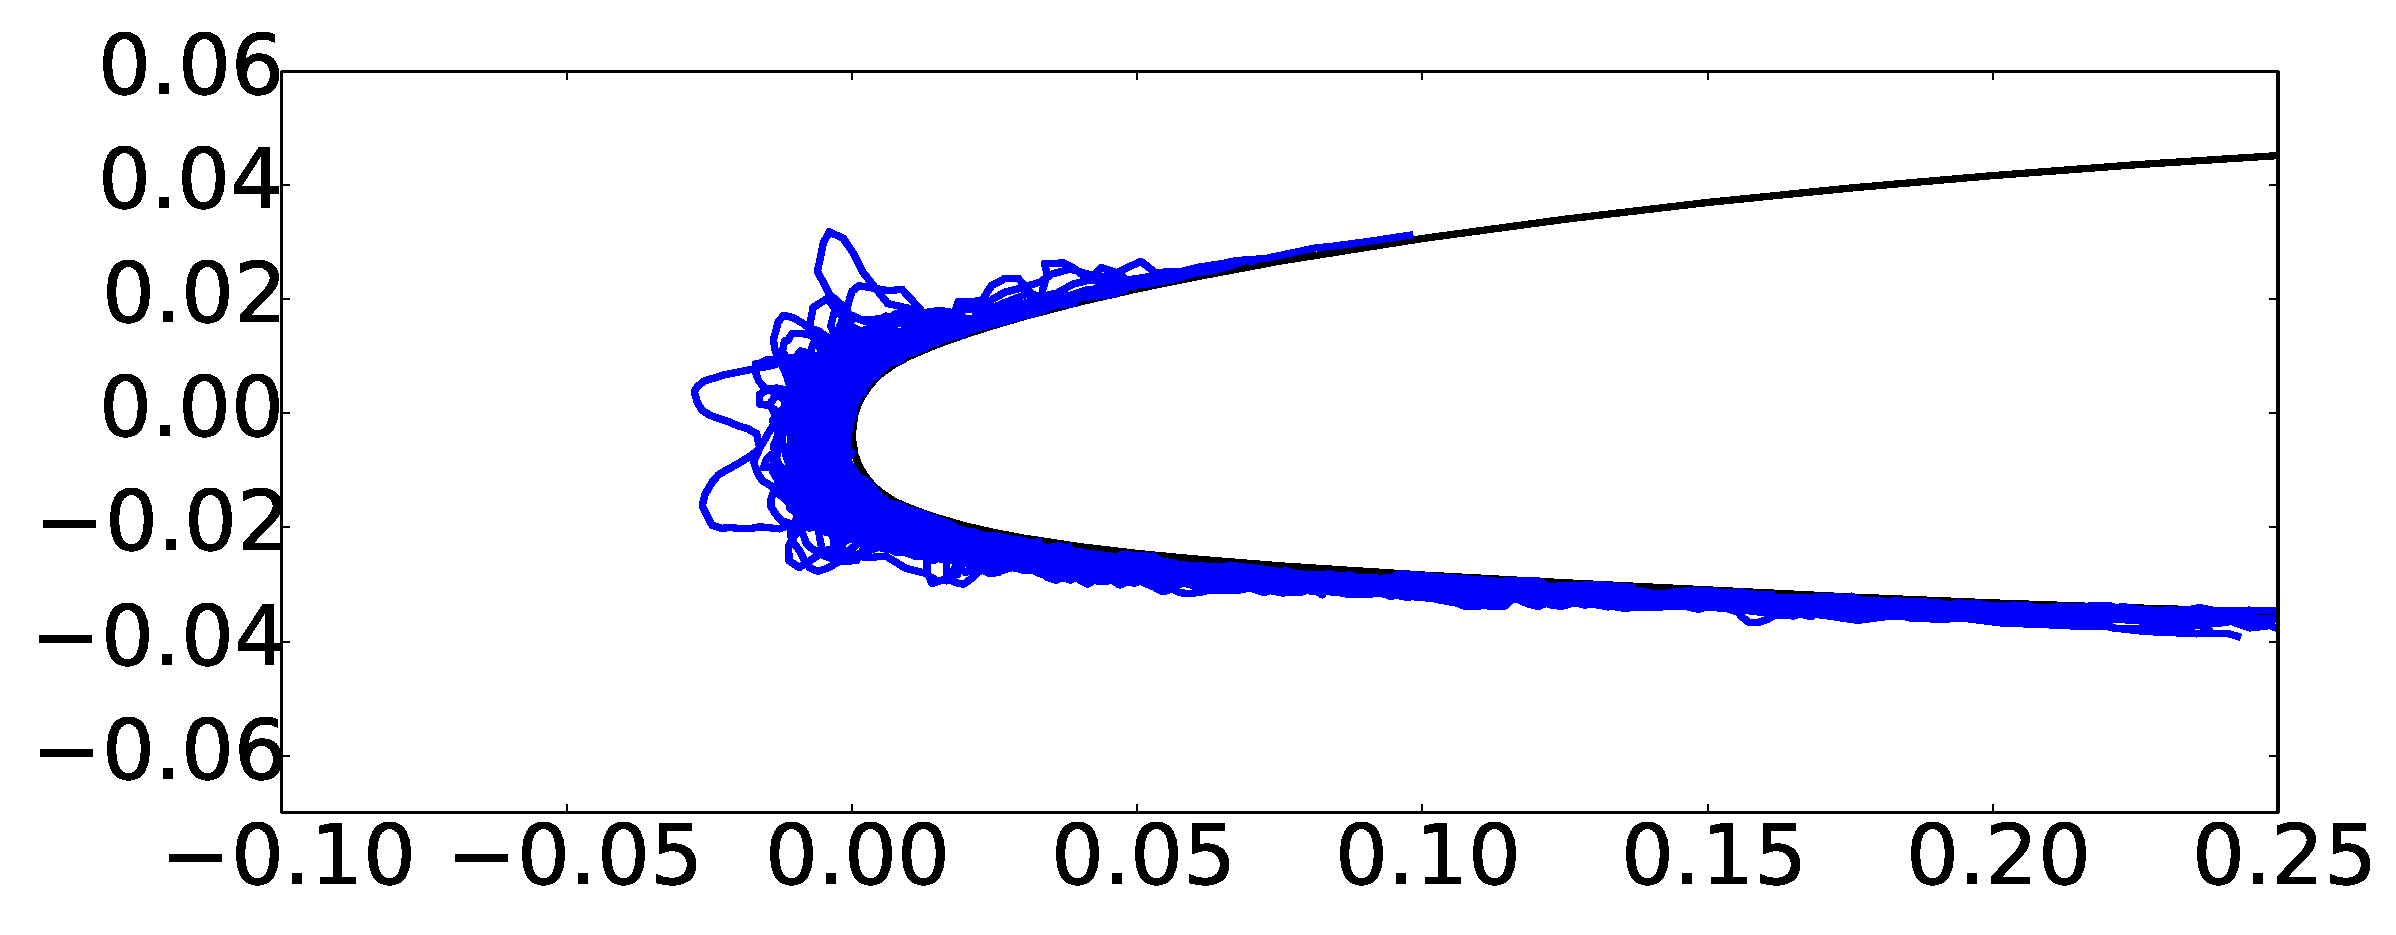
\includegraphics[width=0.45\textwidth]{LaplacianUnconnectedCluster}}
      \caption{$\lambda = 0$}
\end{figure}
\begin{itemize}
\item Unconnected cluster represents smaller and less ``extreme'' shapes
\end{itemize}
\end{frame}
\begin{frame}
\frametitle{Clusters}
\label{sec-3-10}

\vspace*{-0.0cm}\begin{figure}
      \subfigure[Similarity Matrix]{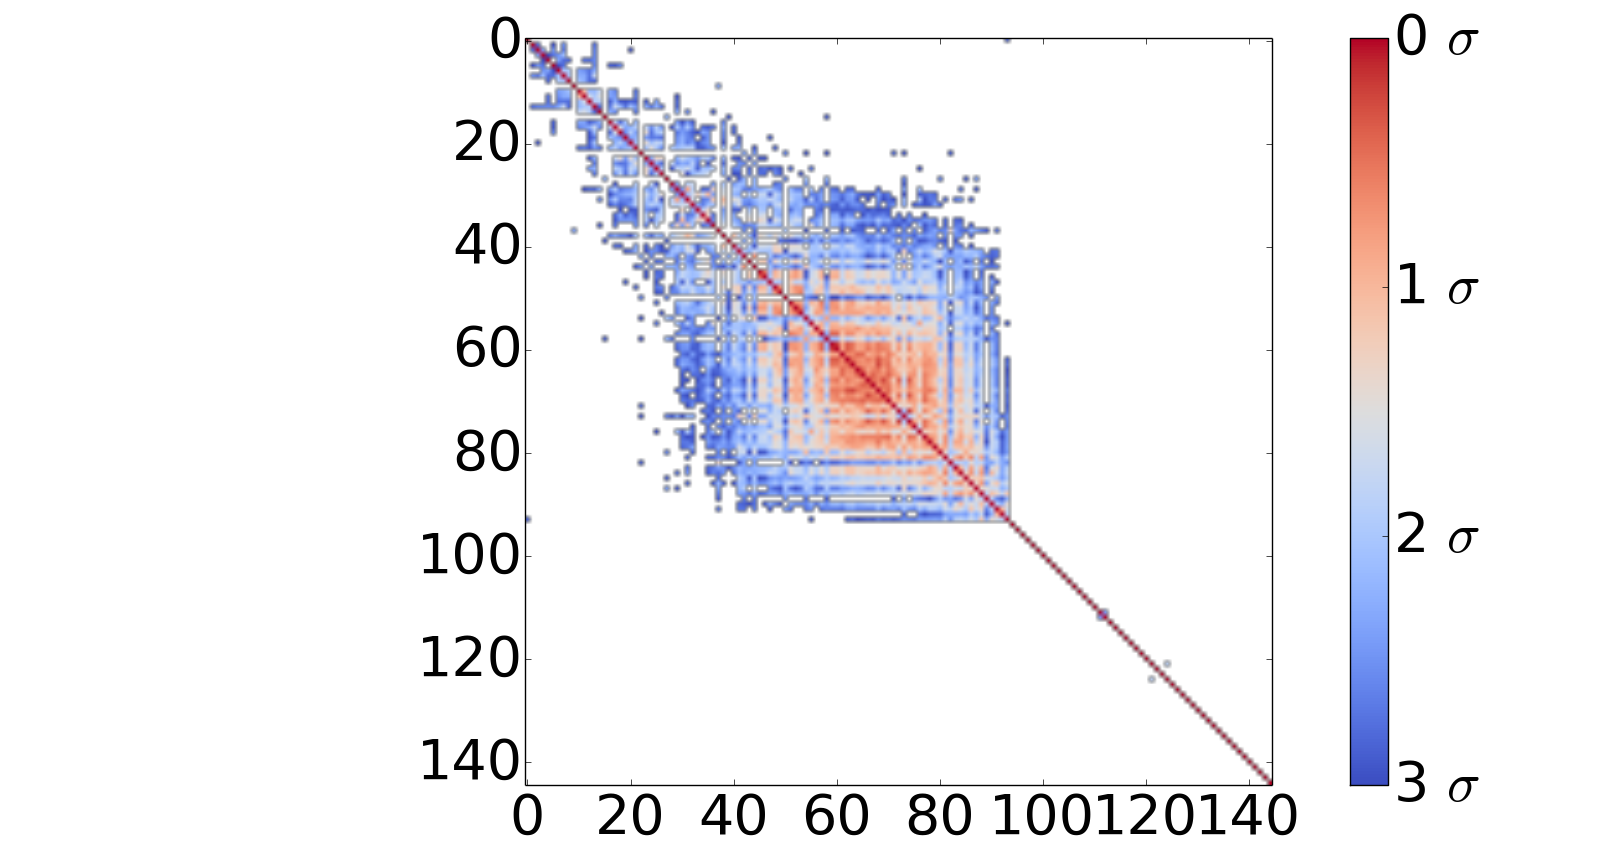
\includegraphics[width=0.45\textwidth]{DistanceMatrixOrdered.png}}
      \subfigure[Ice shapes]{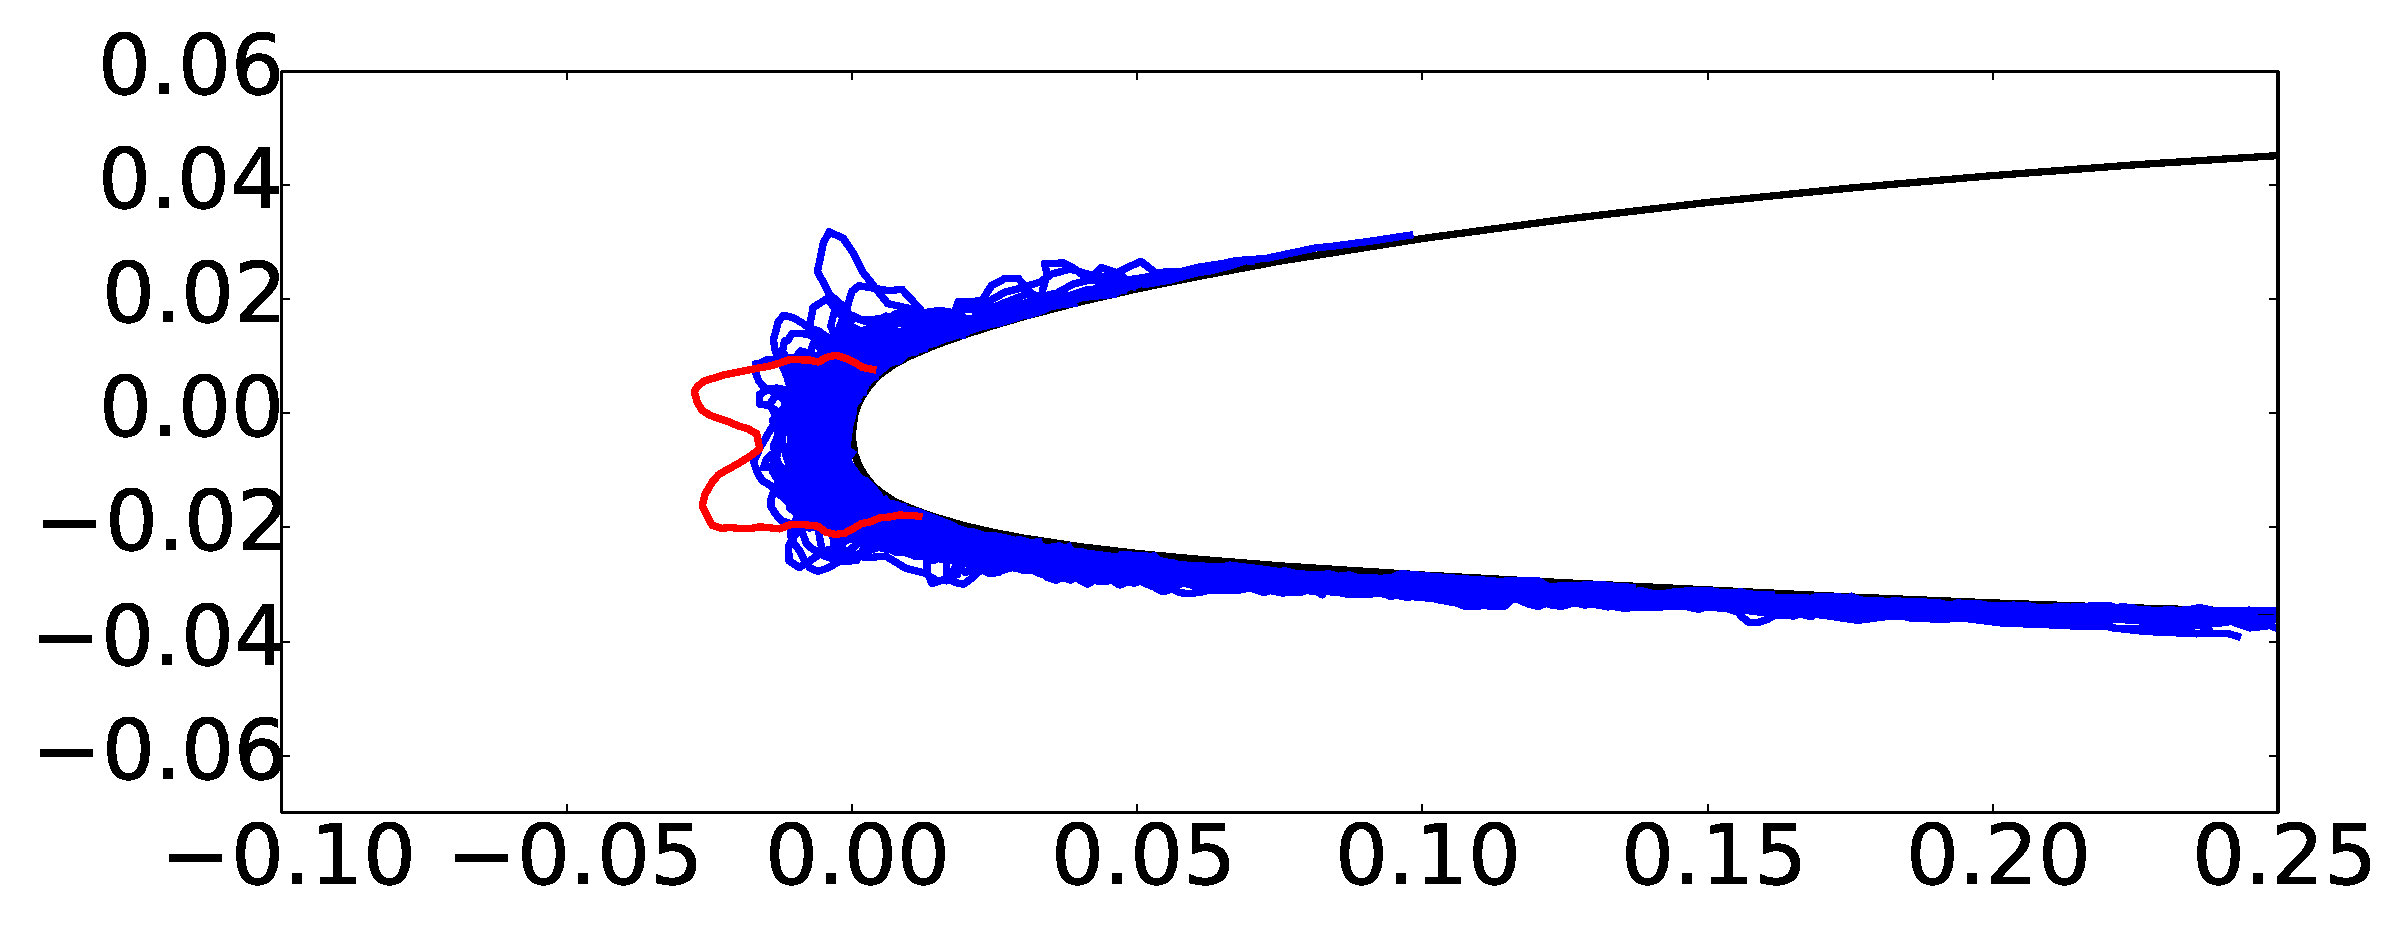
\includegraphics[width=0.45\textwidth]{FiedlerVectorGrouping}}
      \caption{Fiedler vector}
\end{figure}
\begin{itemize}
\item Fiedler vector partitions off single most dissimilar member
\end{itemize}
\end{frame}
\begin{frame}
\frametitle{Clusters}
\label{sec-3-11}

\vspace*{-0.0cm}\begin{figure}
      \subfigure[Similarity Matrix]{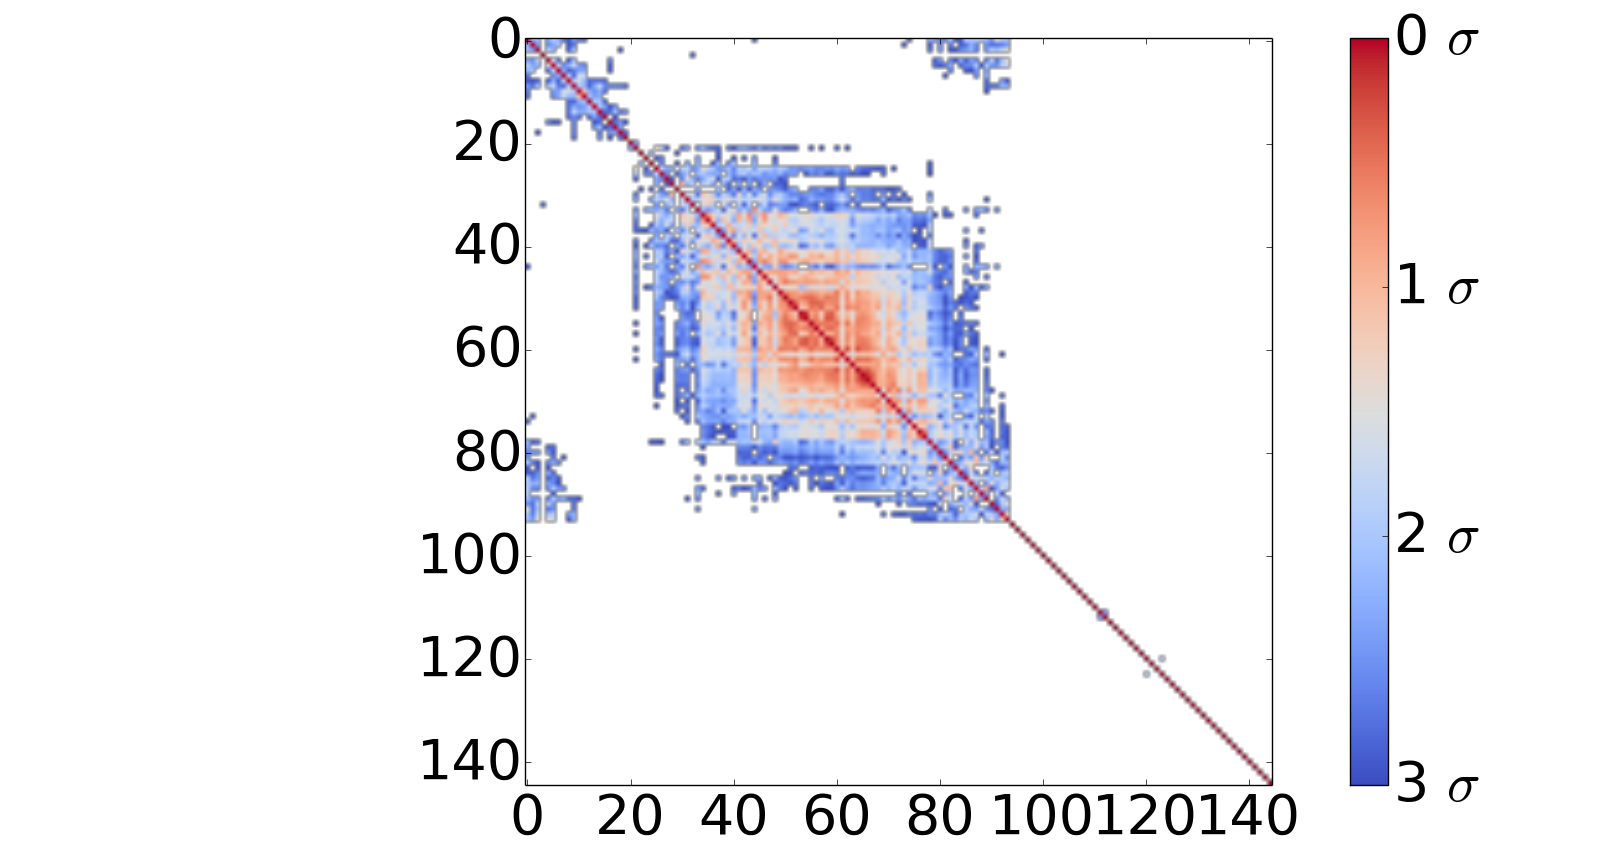
\includegraphics[width=0.45\textwidth]{DistanceMatrixOrdered2.png}}
      \subfigure[Ice shapes]{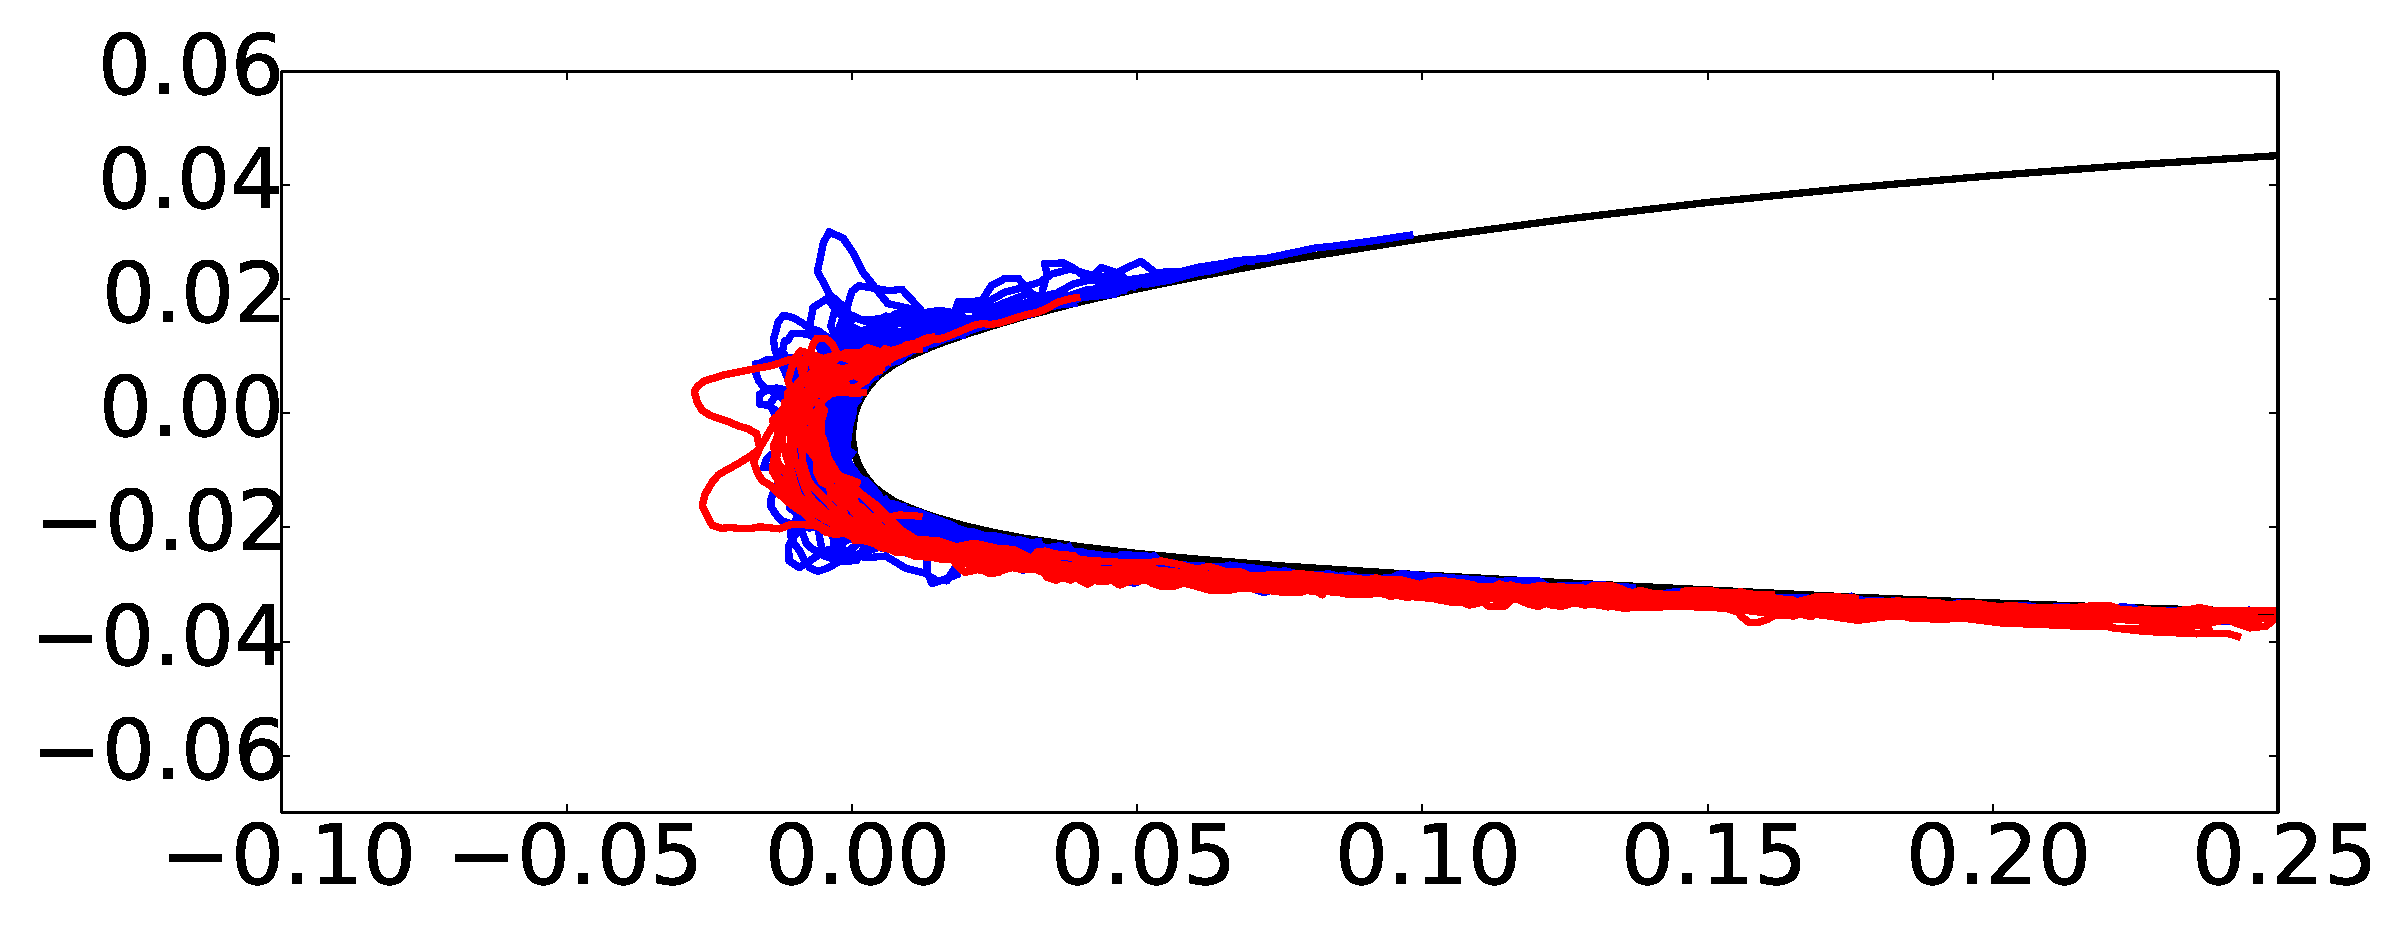
\includegraphics[width=0.45\textwidth]{Fiedler2VectorGrouping}}
      \caption{Next smallest eigenvector}
\end{figure}
\begin{itemize}
\item Next smallest eigenvector separates horn and rime accretion
\end{itemize}
\end{frame}
\begin{frame}
\frametitle{POD Coordinates}
\label{sec-3-12}

\vspace*{-0.0cm}\begin{figure}
      \subfigure[POD coordinates]{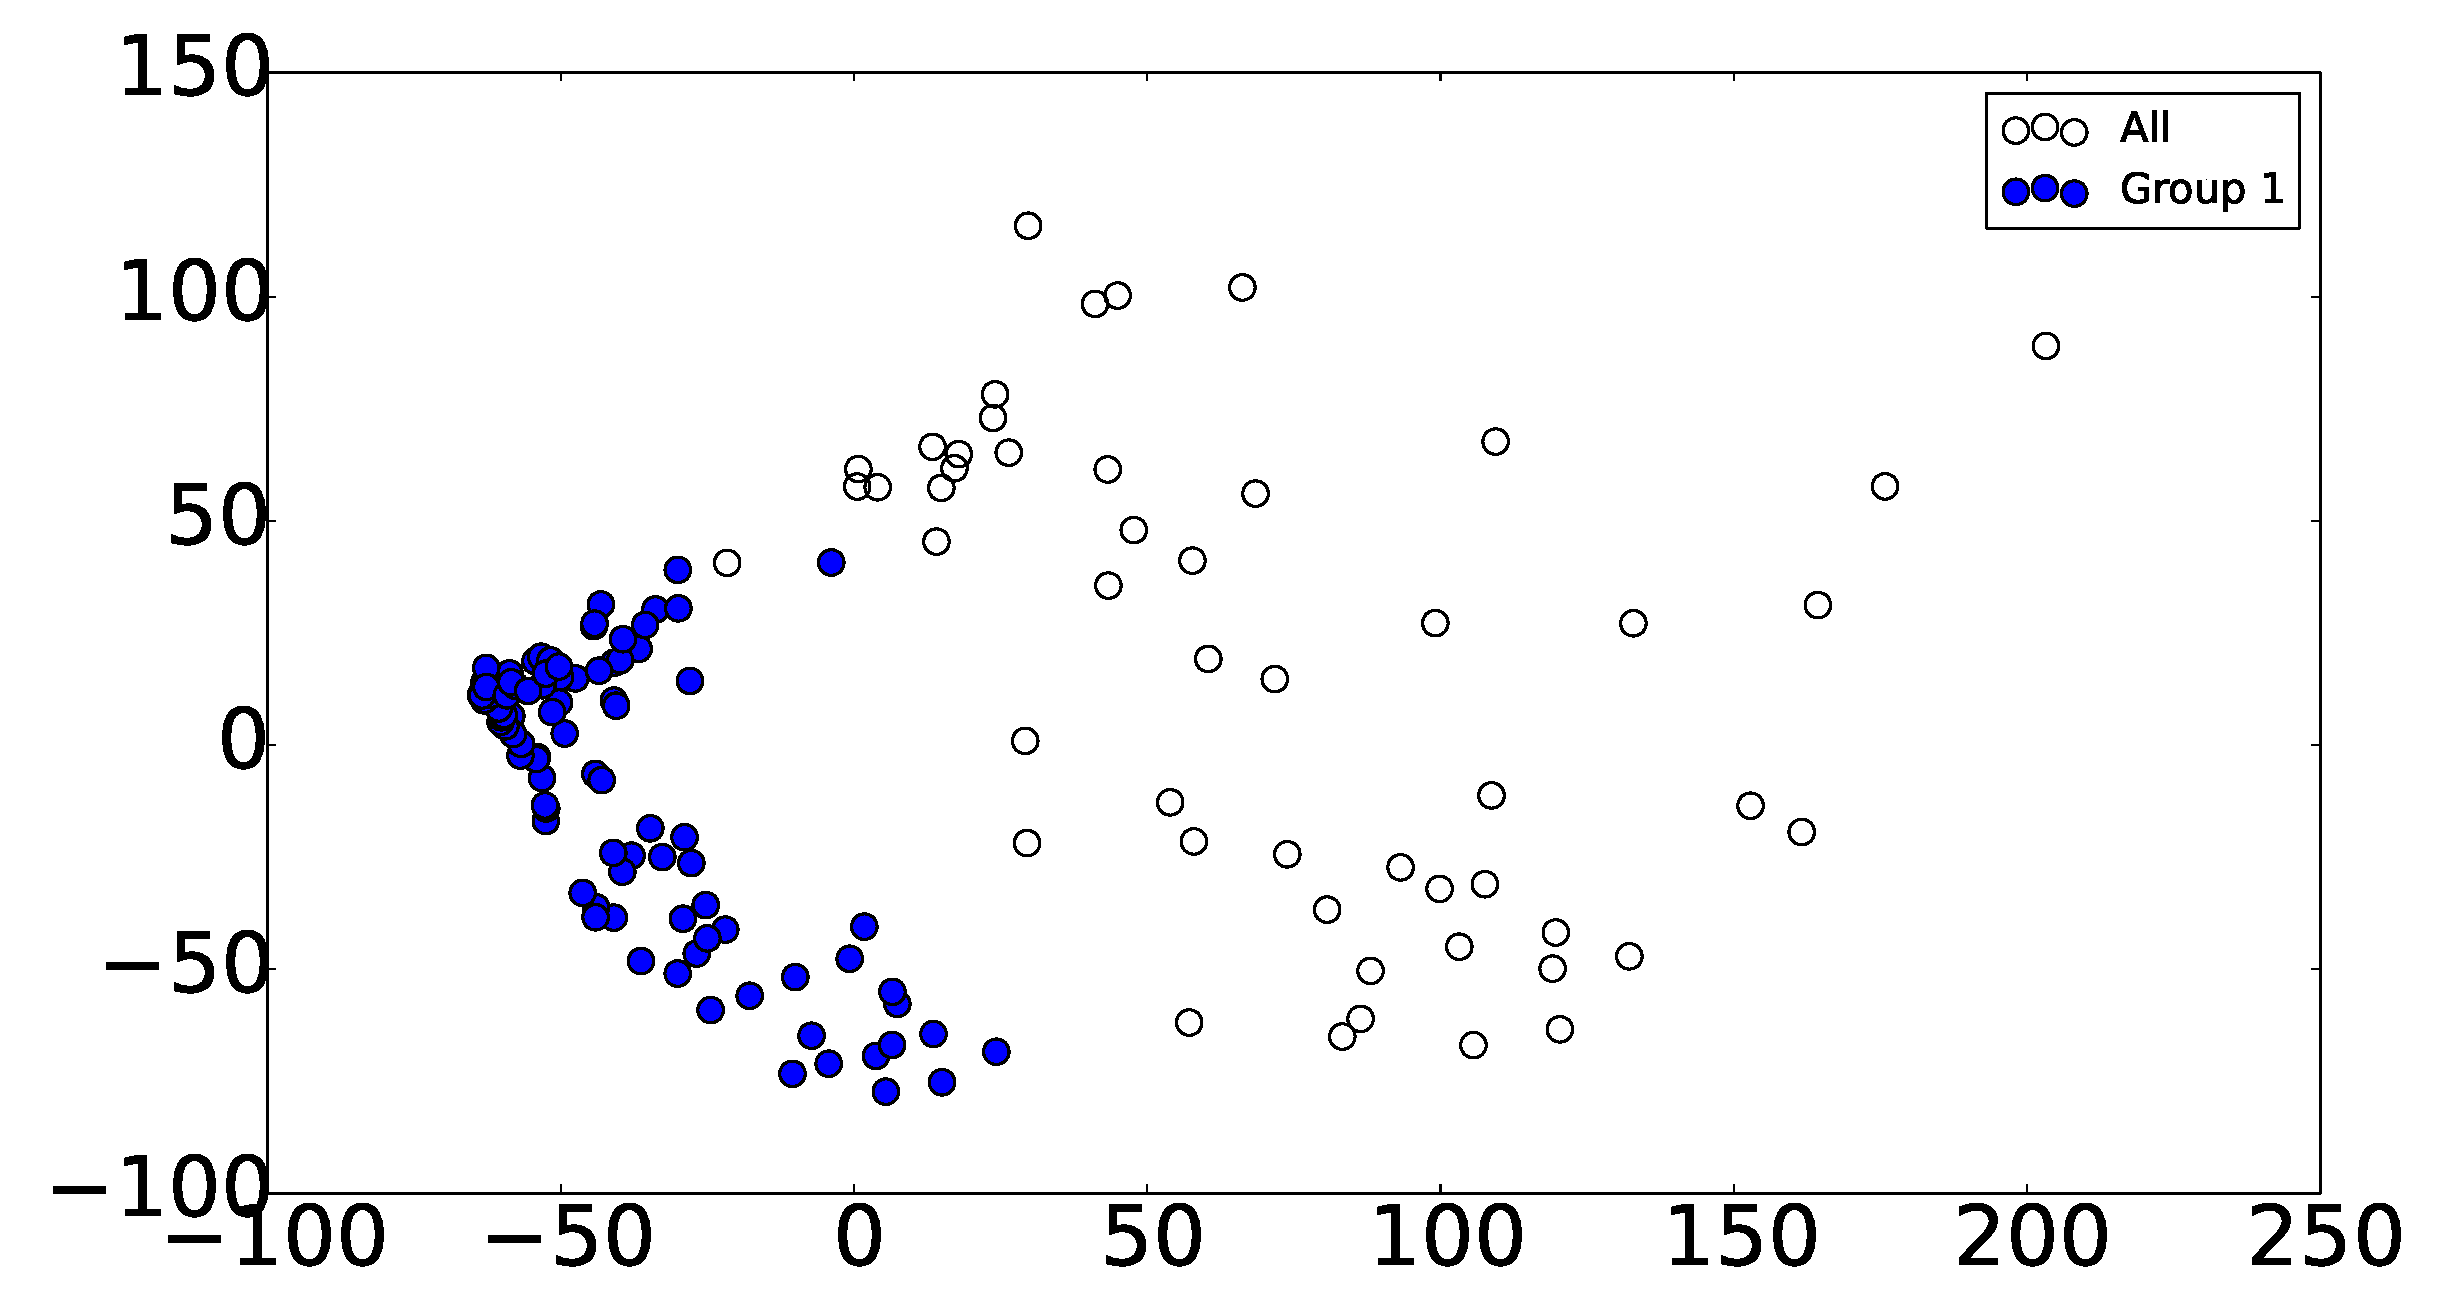
\includegraphics[width=0.5\textwidth]{ClusterPODcoords}}
      \subfigure[Ice shapes]{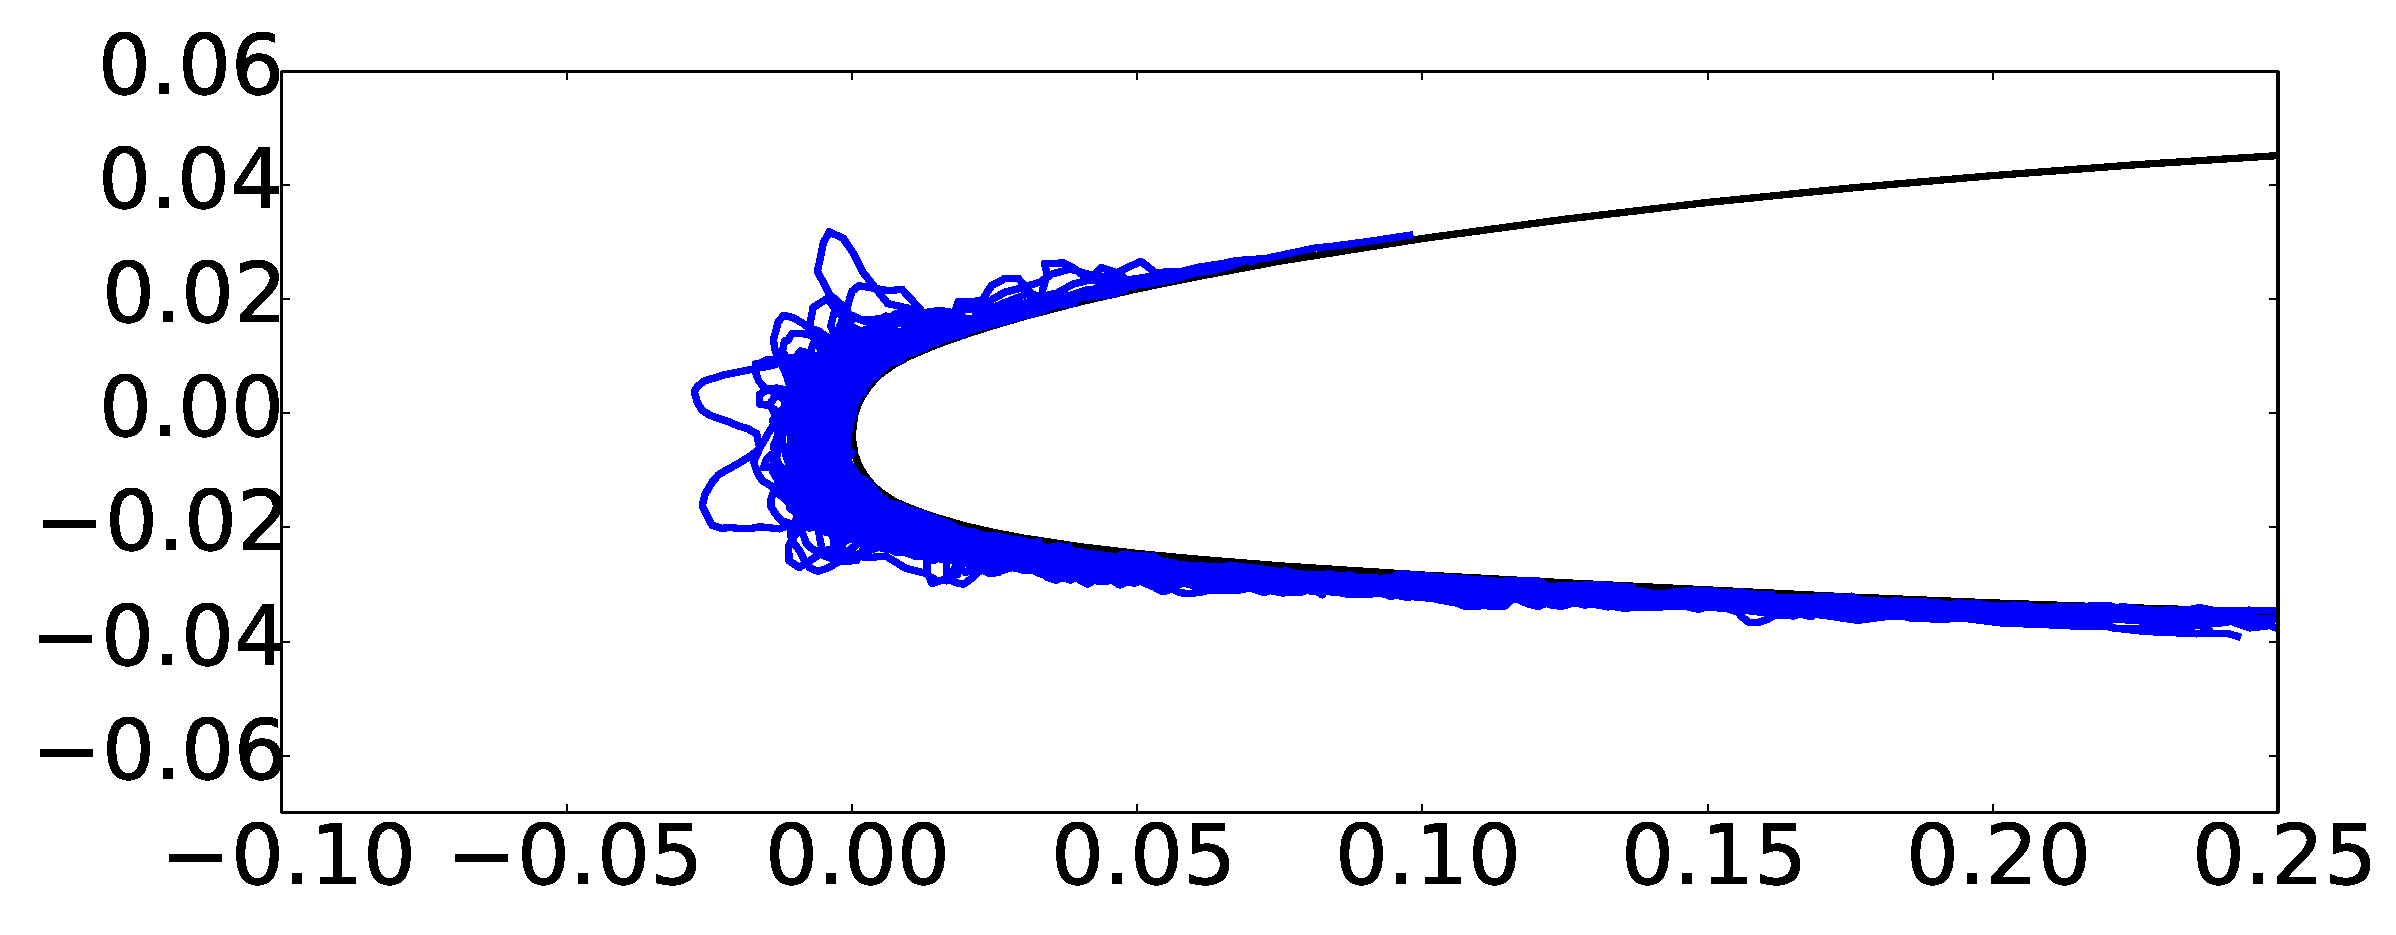
\includegraphics[width=0.5\textwidth]{LaplacianUnconnectedCluster}}
      \caption{$\lambda = 0$}
\end{figure}
\end{frame}
\begin{frame}
\frametitle{POD Coordinates}
\label{sec-3-13}

\vspace*{-0.0cm}\begin{figure}
      \subfigure[POD coordinates]{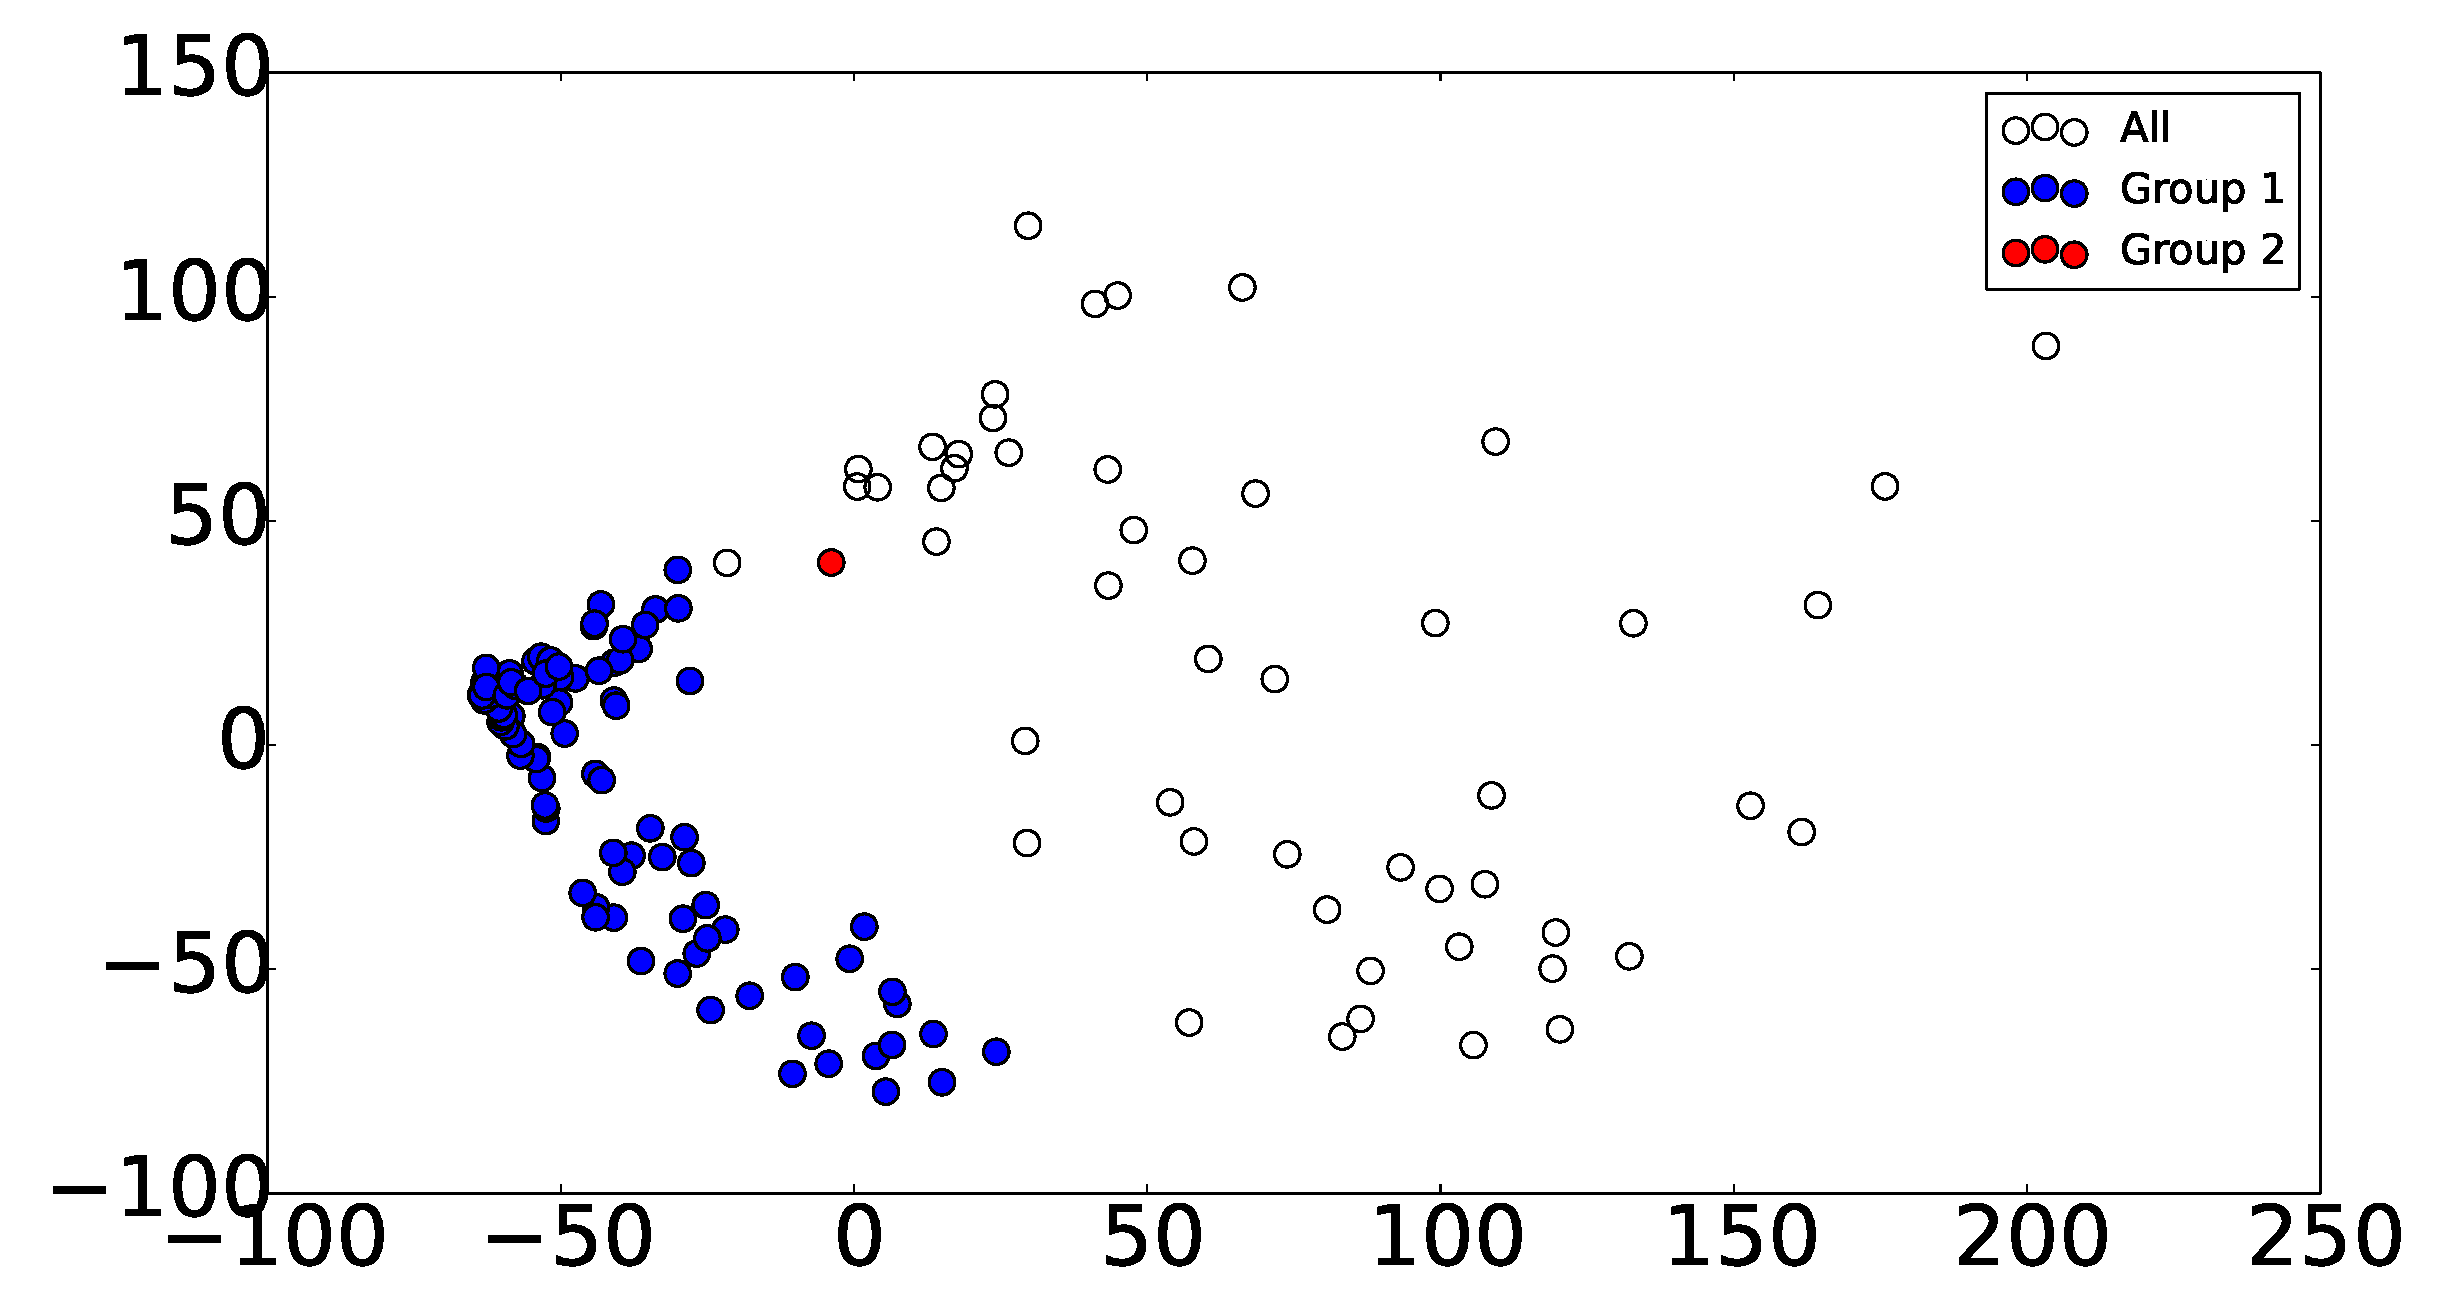
\includegraphics[width=0.5\textwidth]{FiedlerVectorPODcoords}}
      \subfigure[Ice shapes]{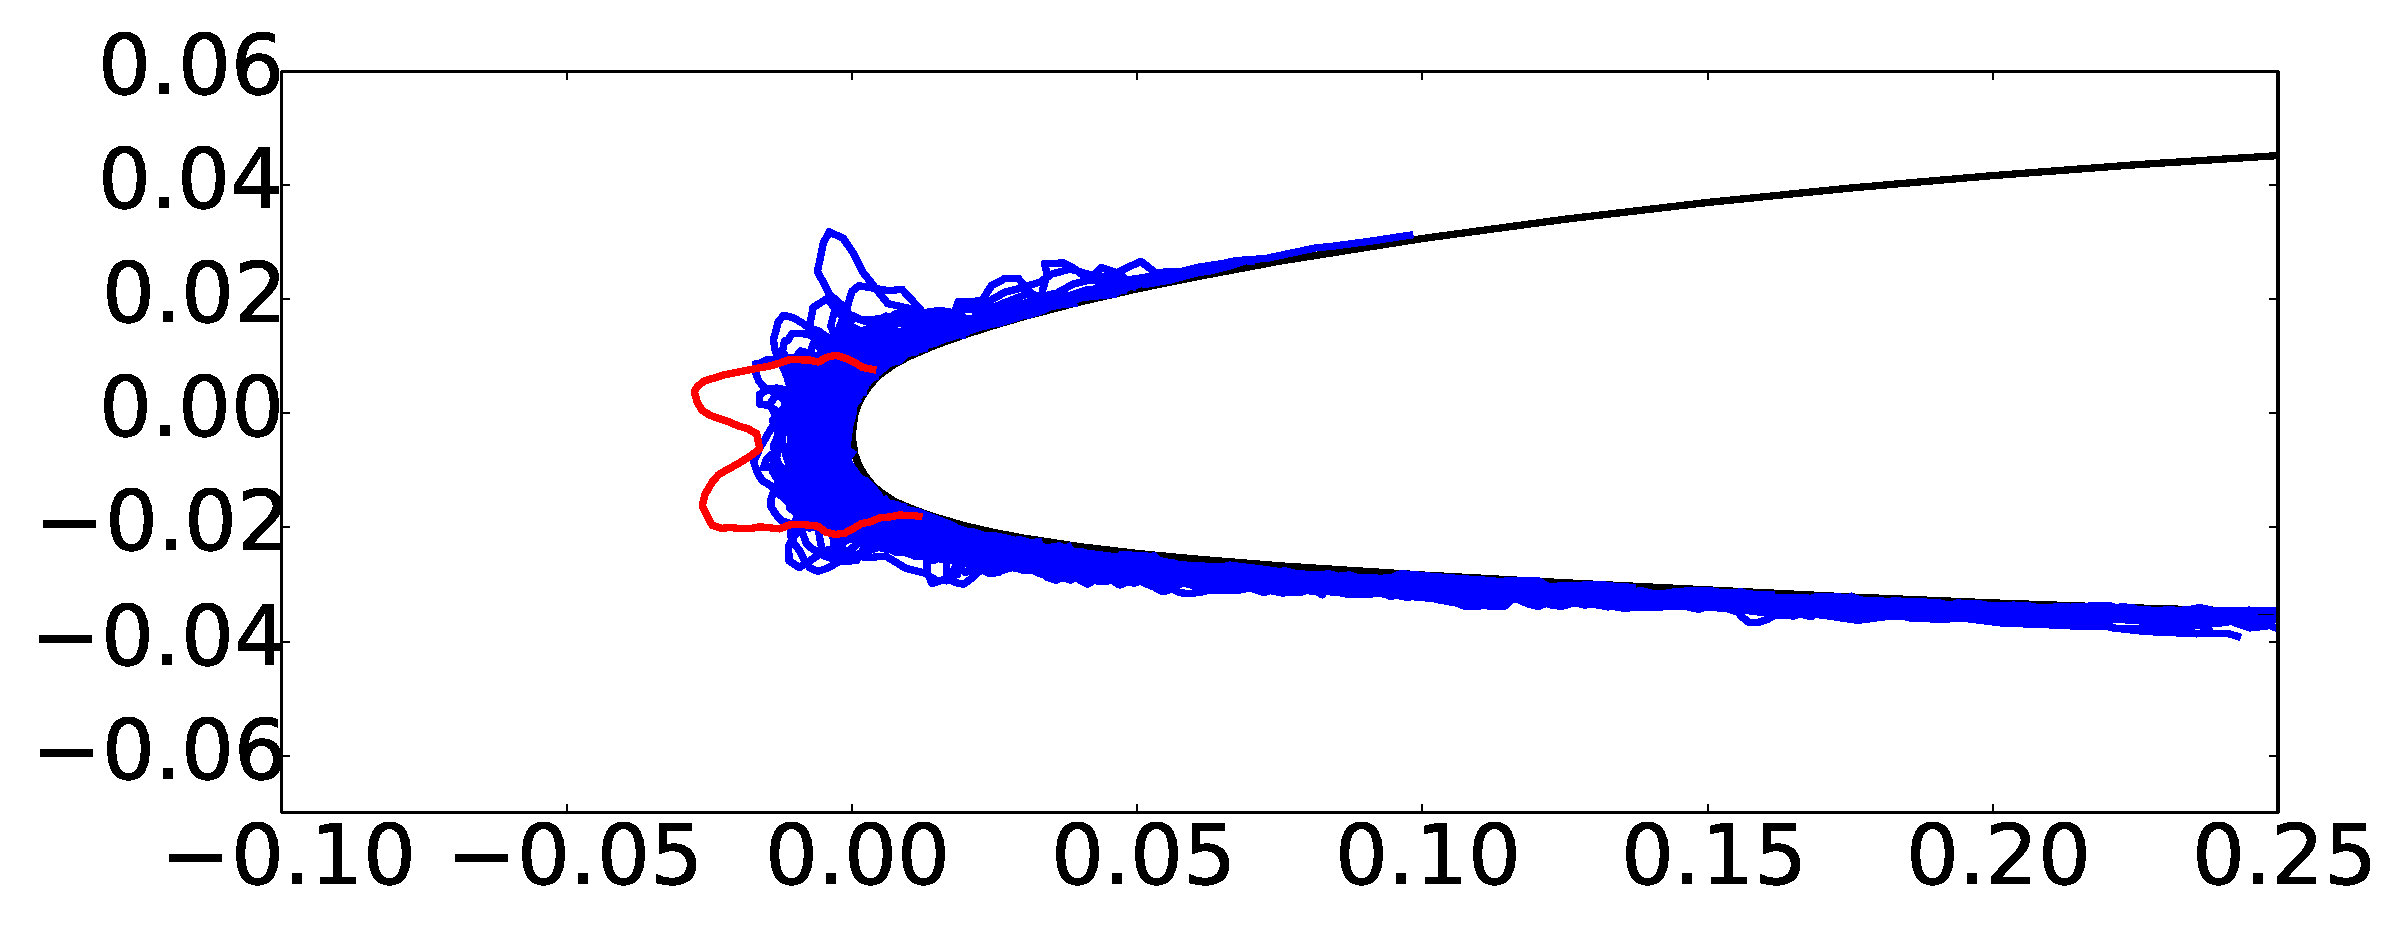
\includegraphics[width=0.5\textwidth]{FiedlerVectorGrouping}}
      \caption{Fiedler vector}
\end{figure}
\end{frame}
\begin{frame}
\frametitle{POD Coordinates}
\label{sec-3-14}

\vspace*{-0.0cm}\begin{figure}
      \subfigure[POD coordinates]{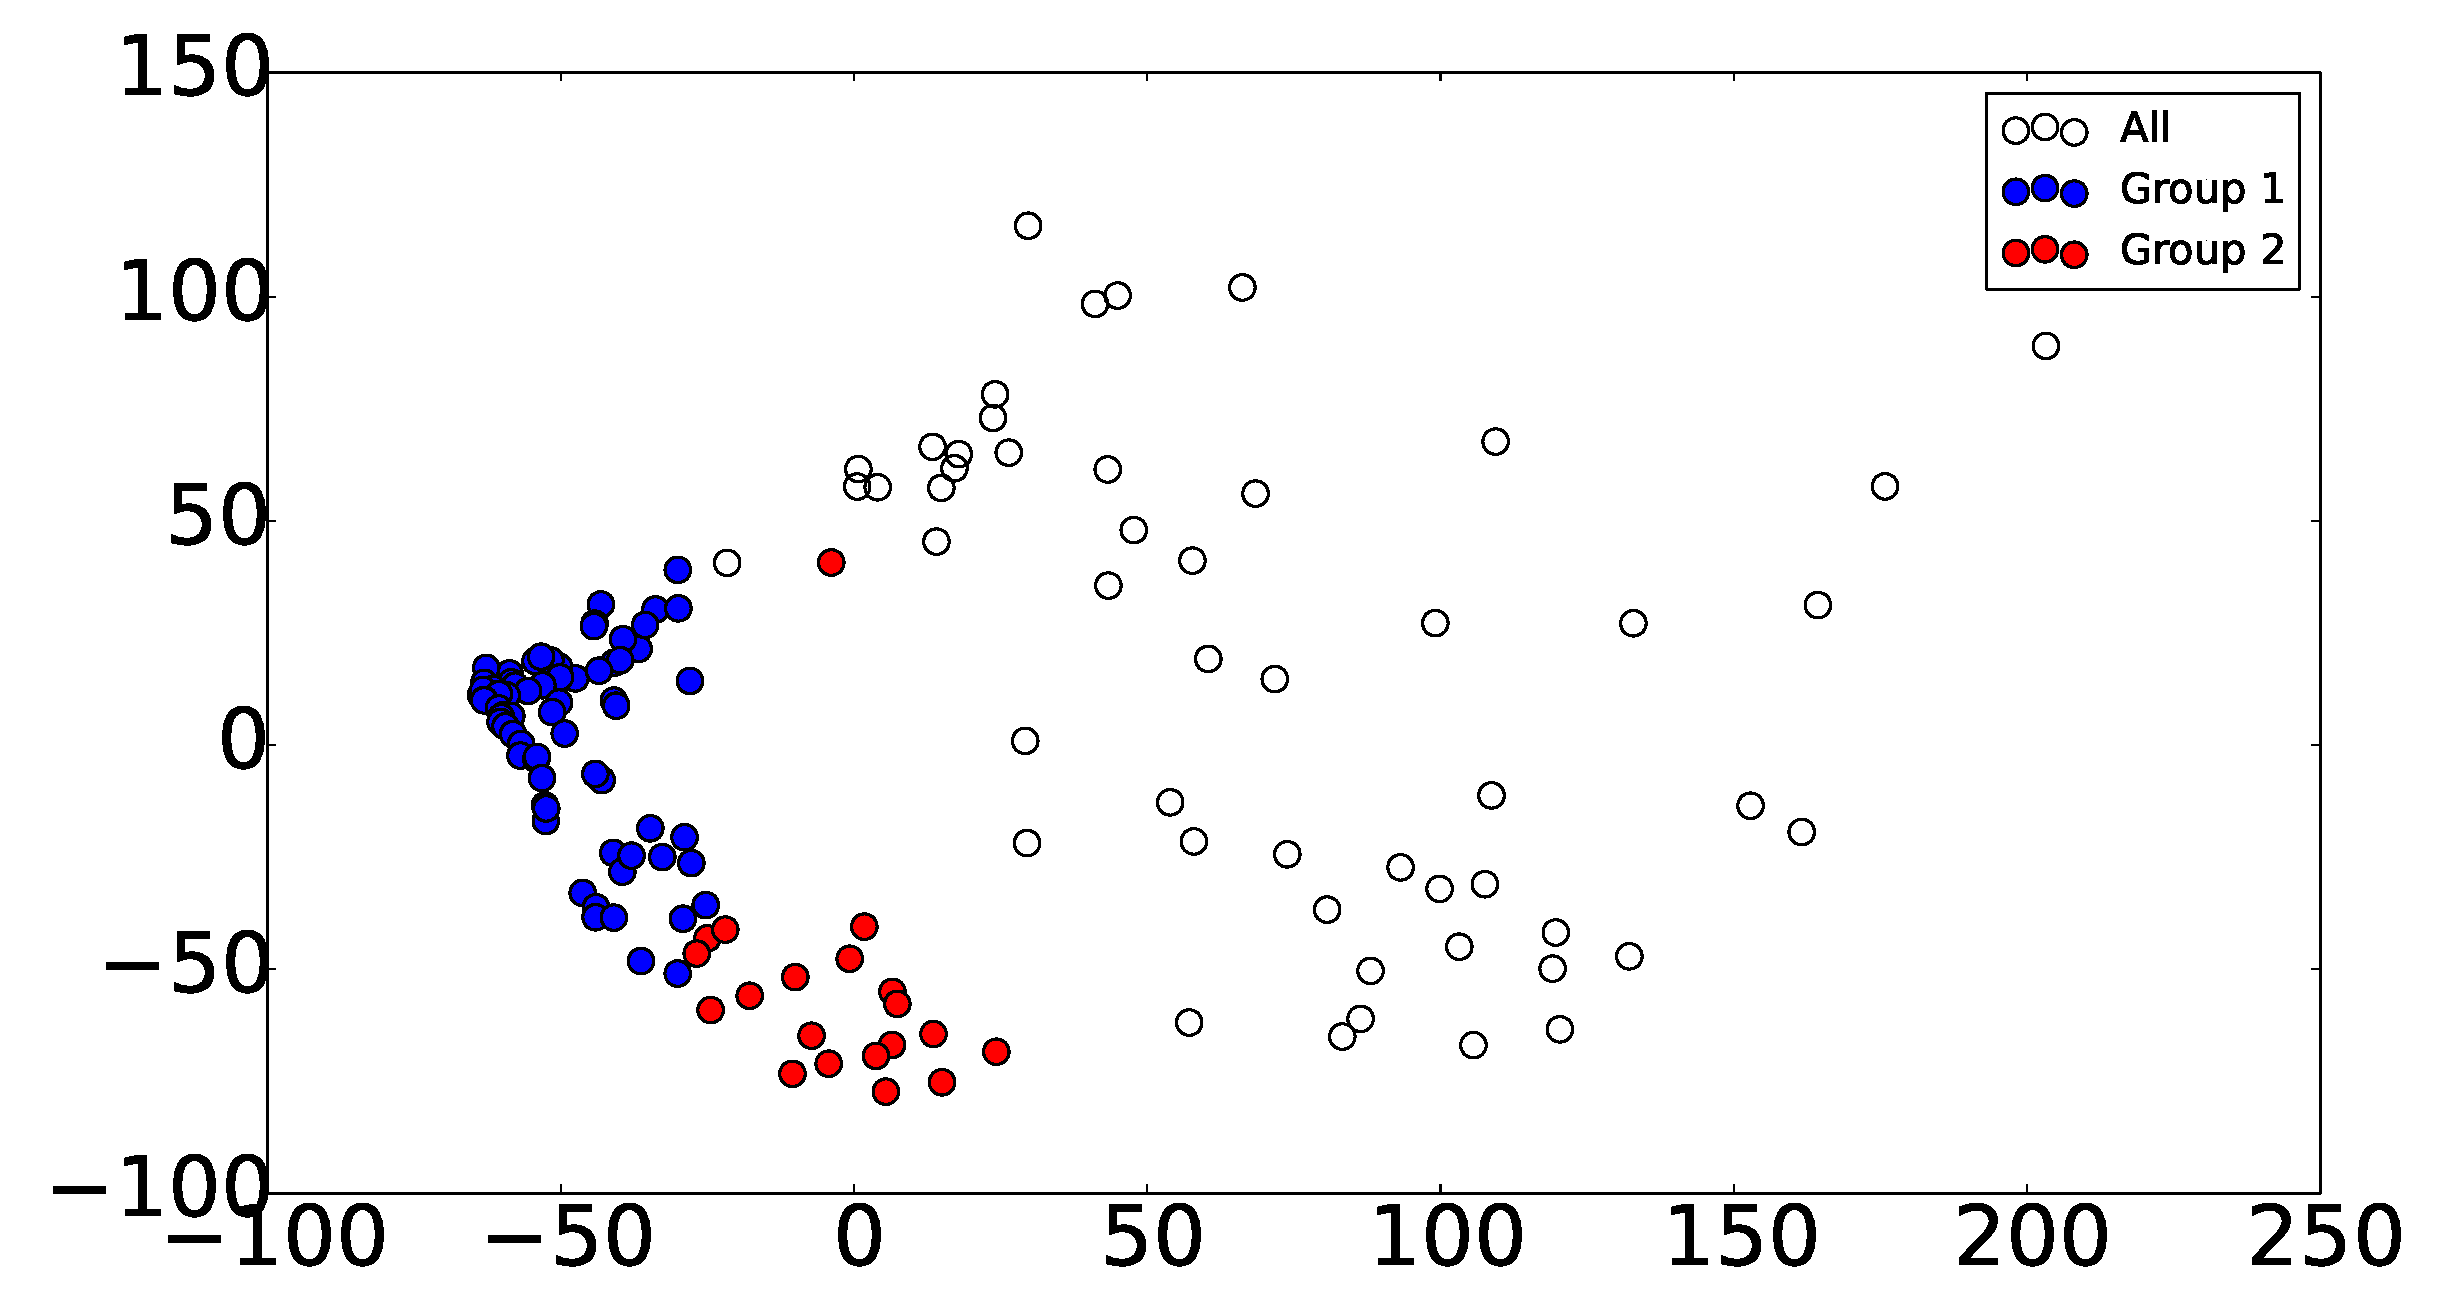
\includegraphics[width=0.5\textwidth]{Fiedler2VectorPODcoords}}
      \subfigure[Ice shapes]{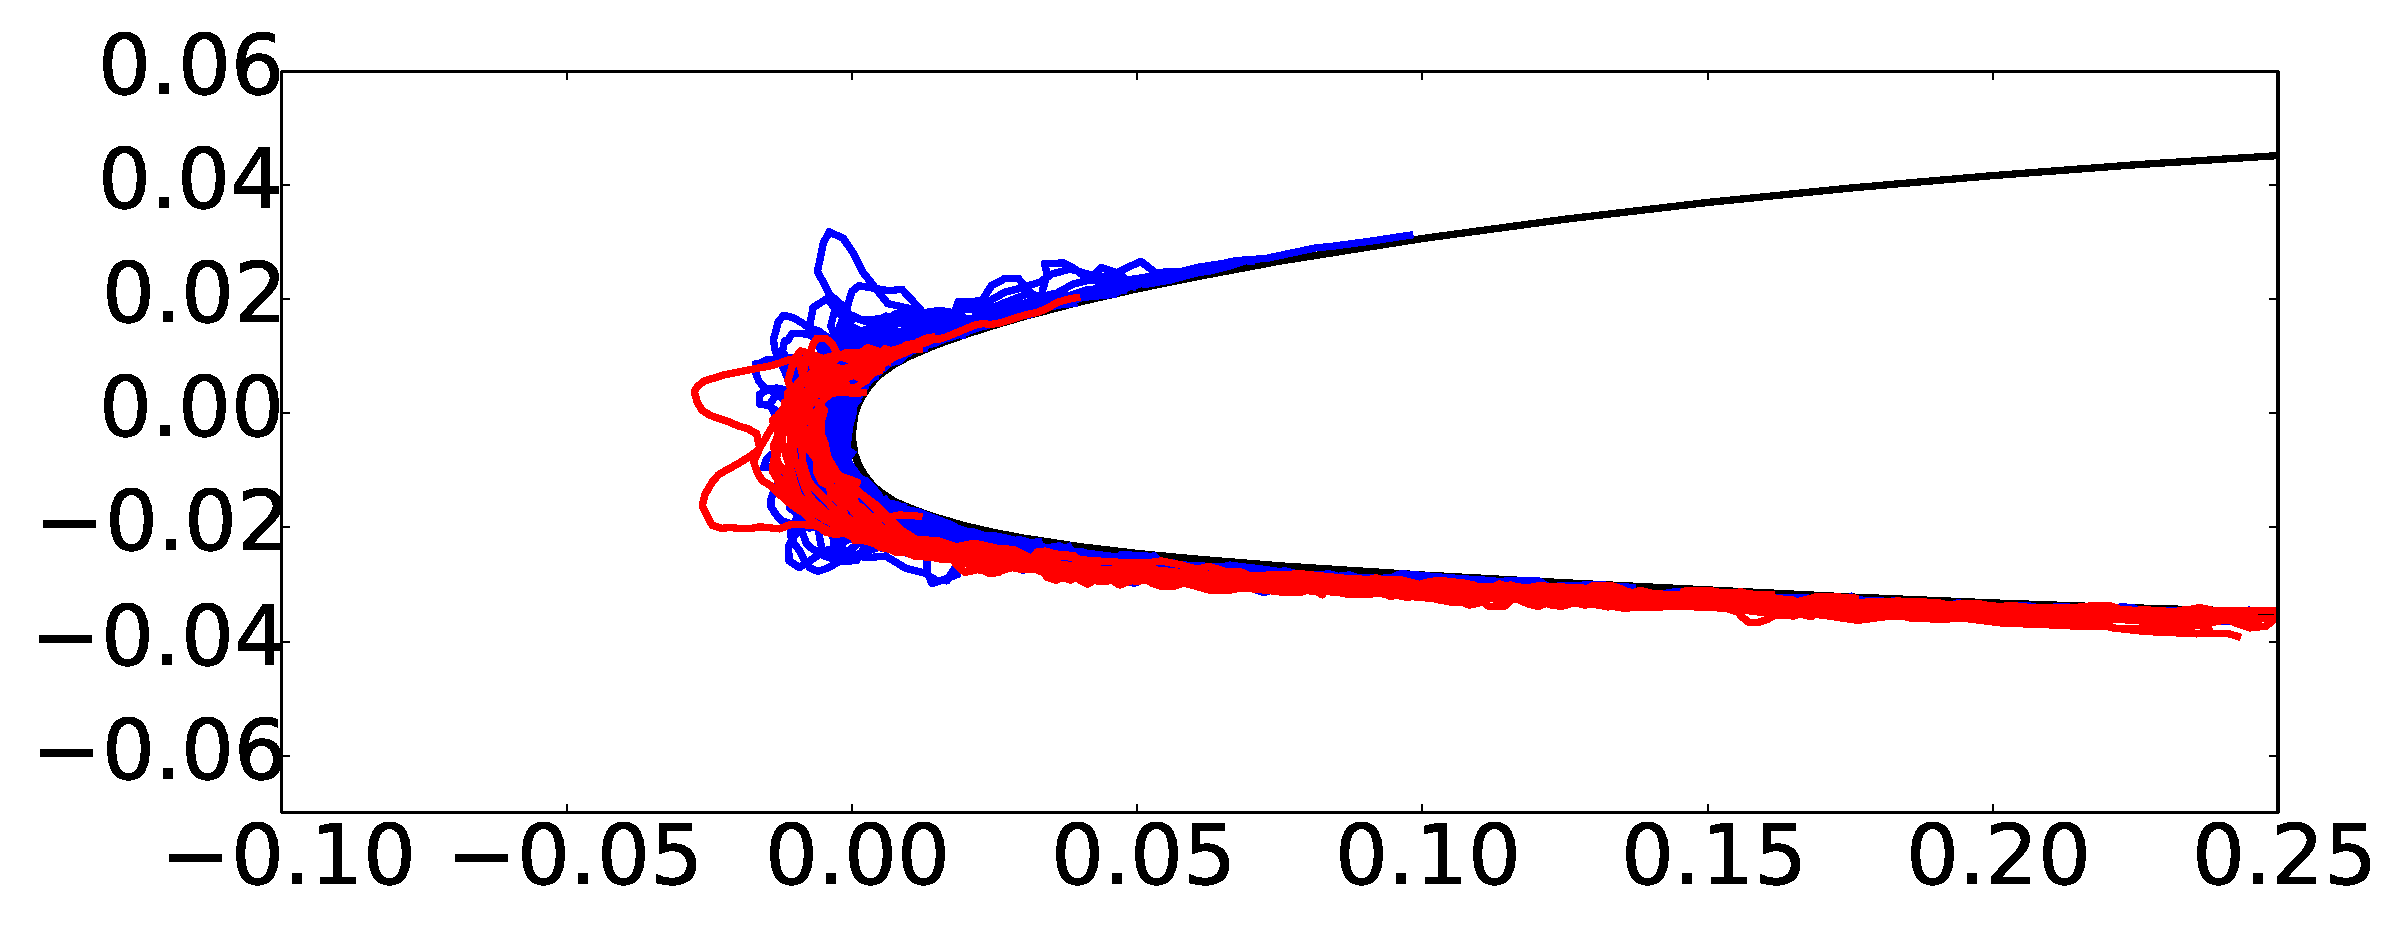
\includegraphics[width=0.5\textwidth]{Fiedler2VectorGrouping}}
      \caption{Next smallest eigenvector}
\end{figure}
\end{frame}
\begin{frame}
\frametitle{Cluster Modeling}
\label{sec-3-15}

\vspace*{-0.75cm}\begin{figure}
      \subfigure[$S$-Coordinates]{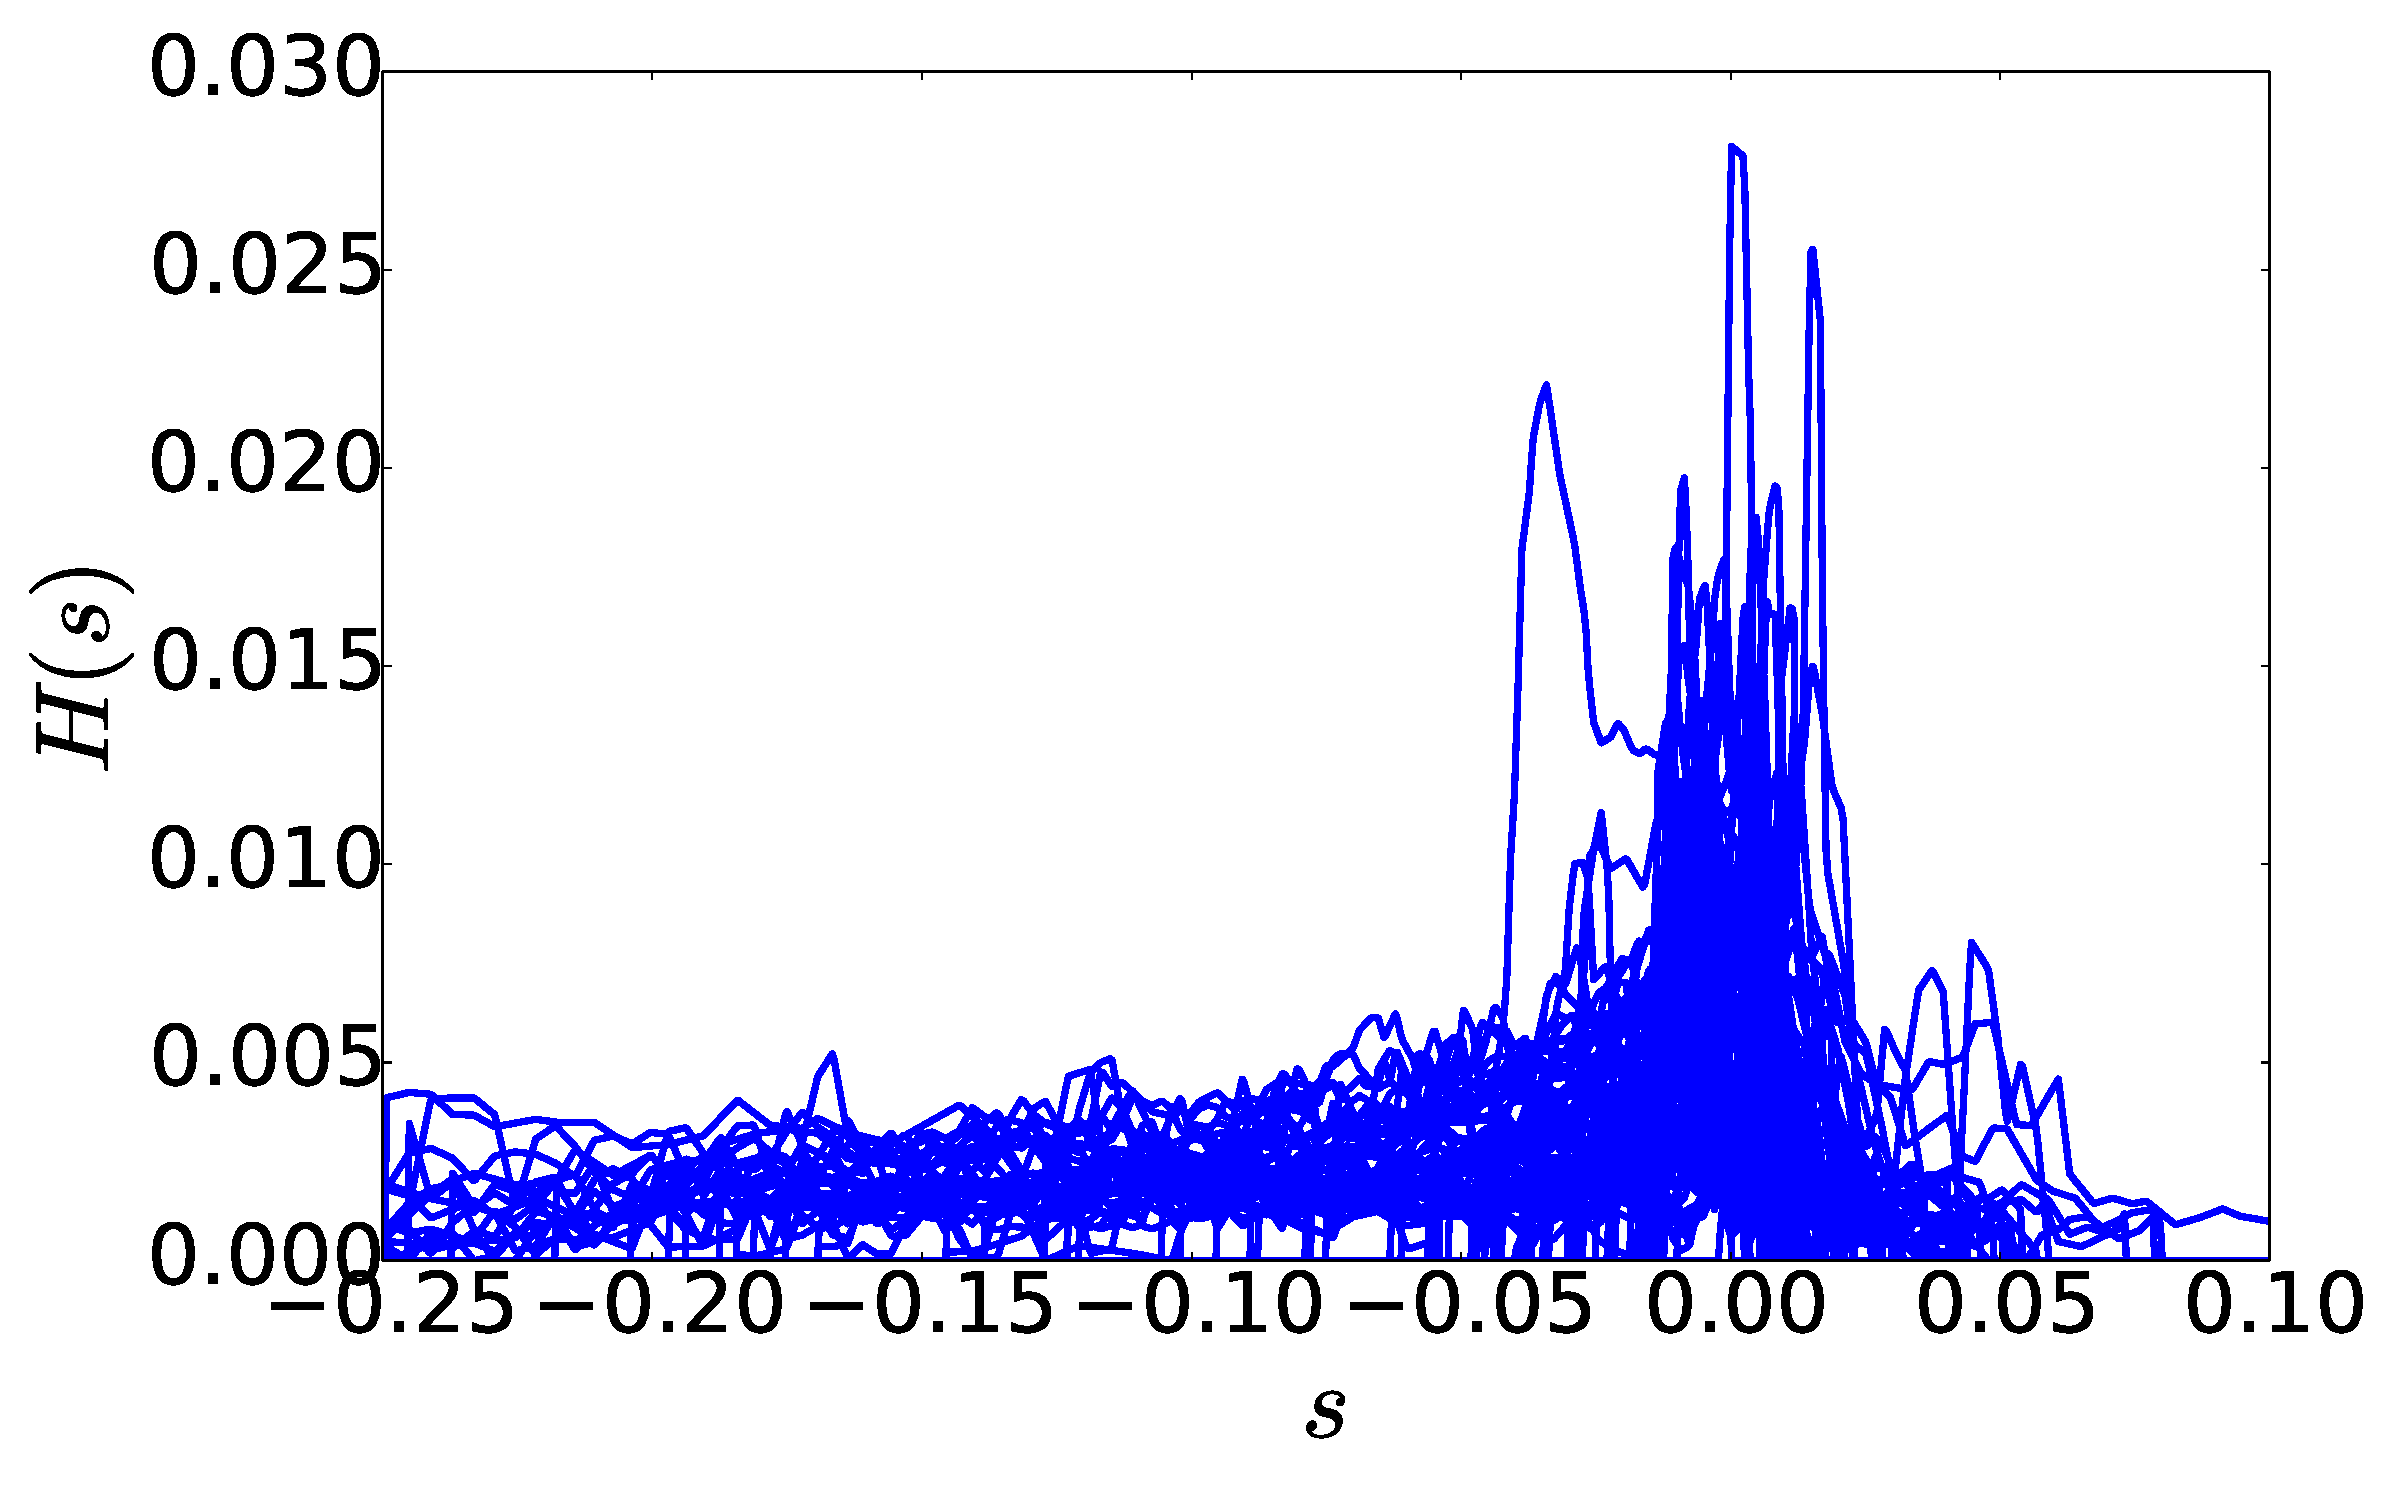
\includegraphics[width=0.35\textwidth]{ScoordsCluster1}}
      \subfigure[POD Eigenvalues]{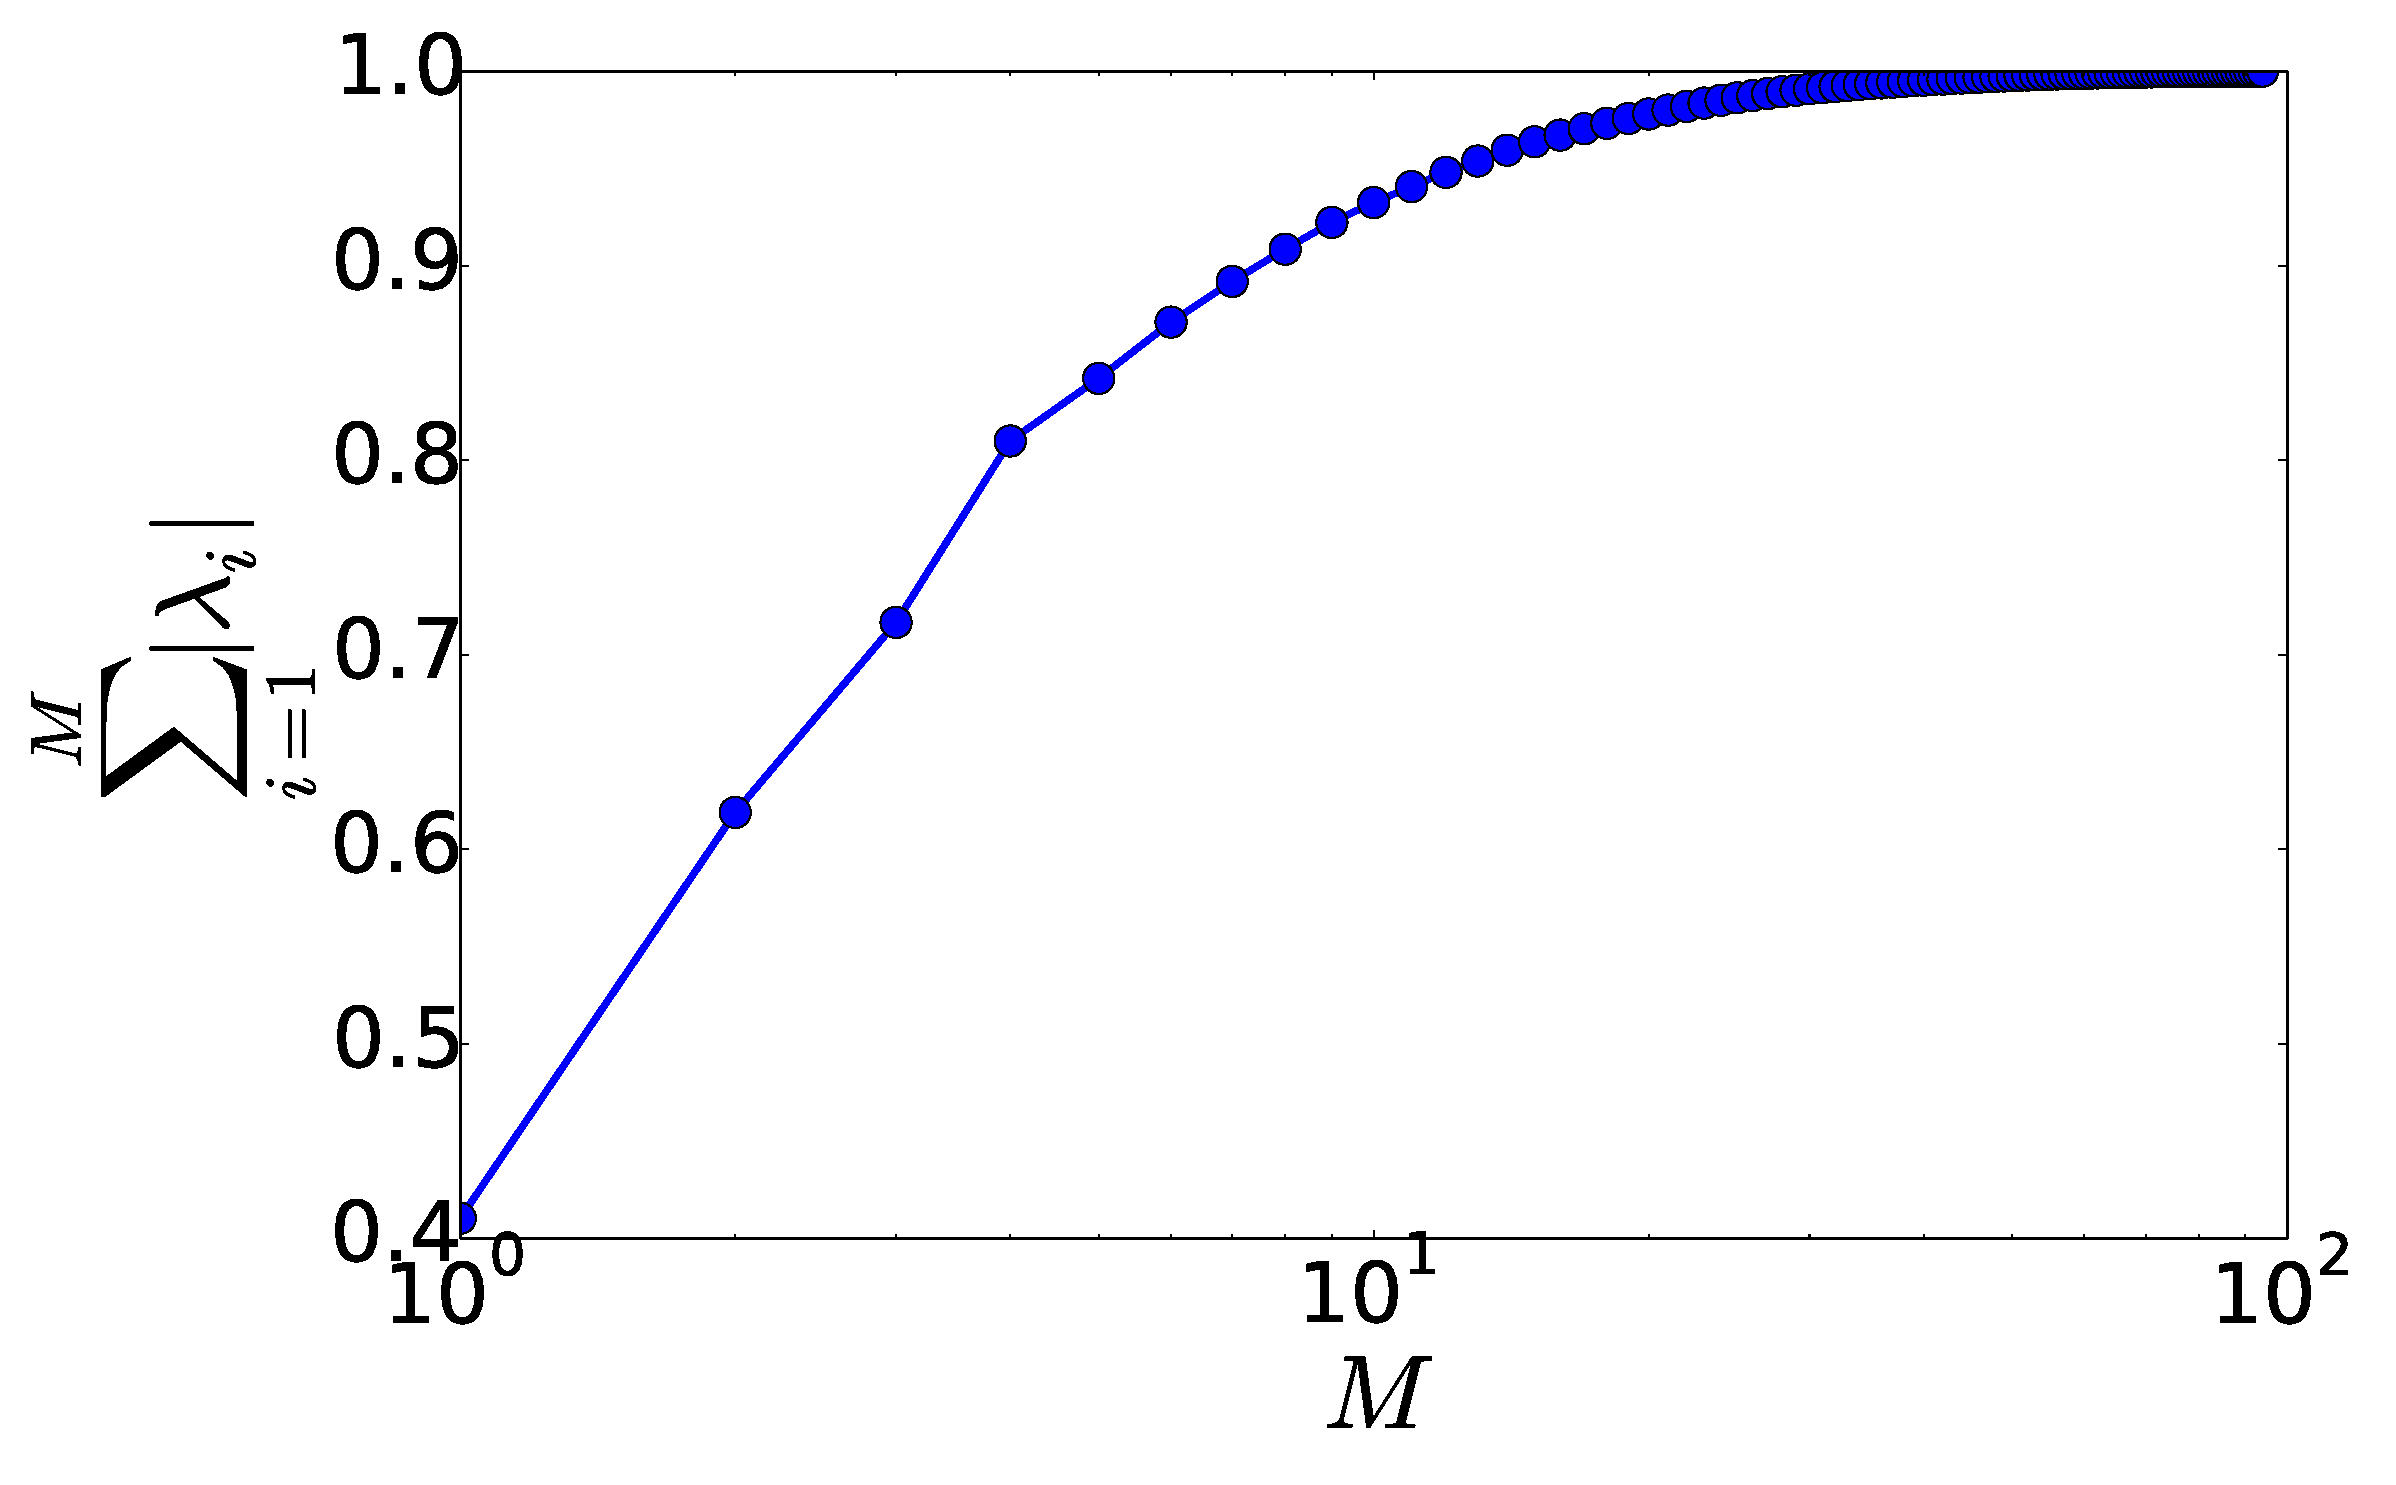
\includegraphics[width=0.35\textwidth]{PODevalsCluster1}}
      \subfigure[Mean]{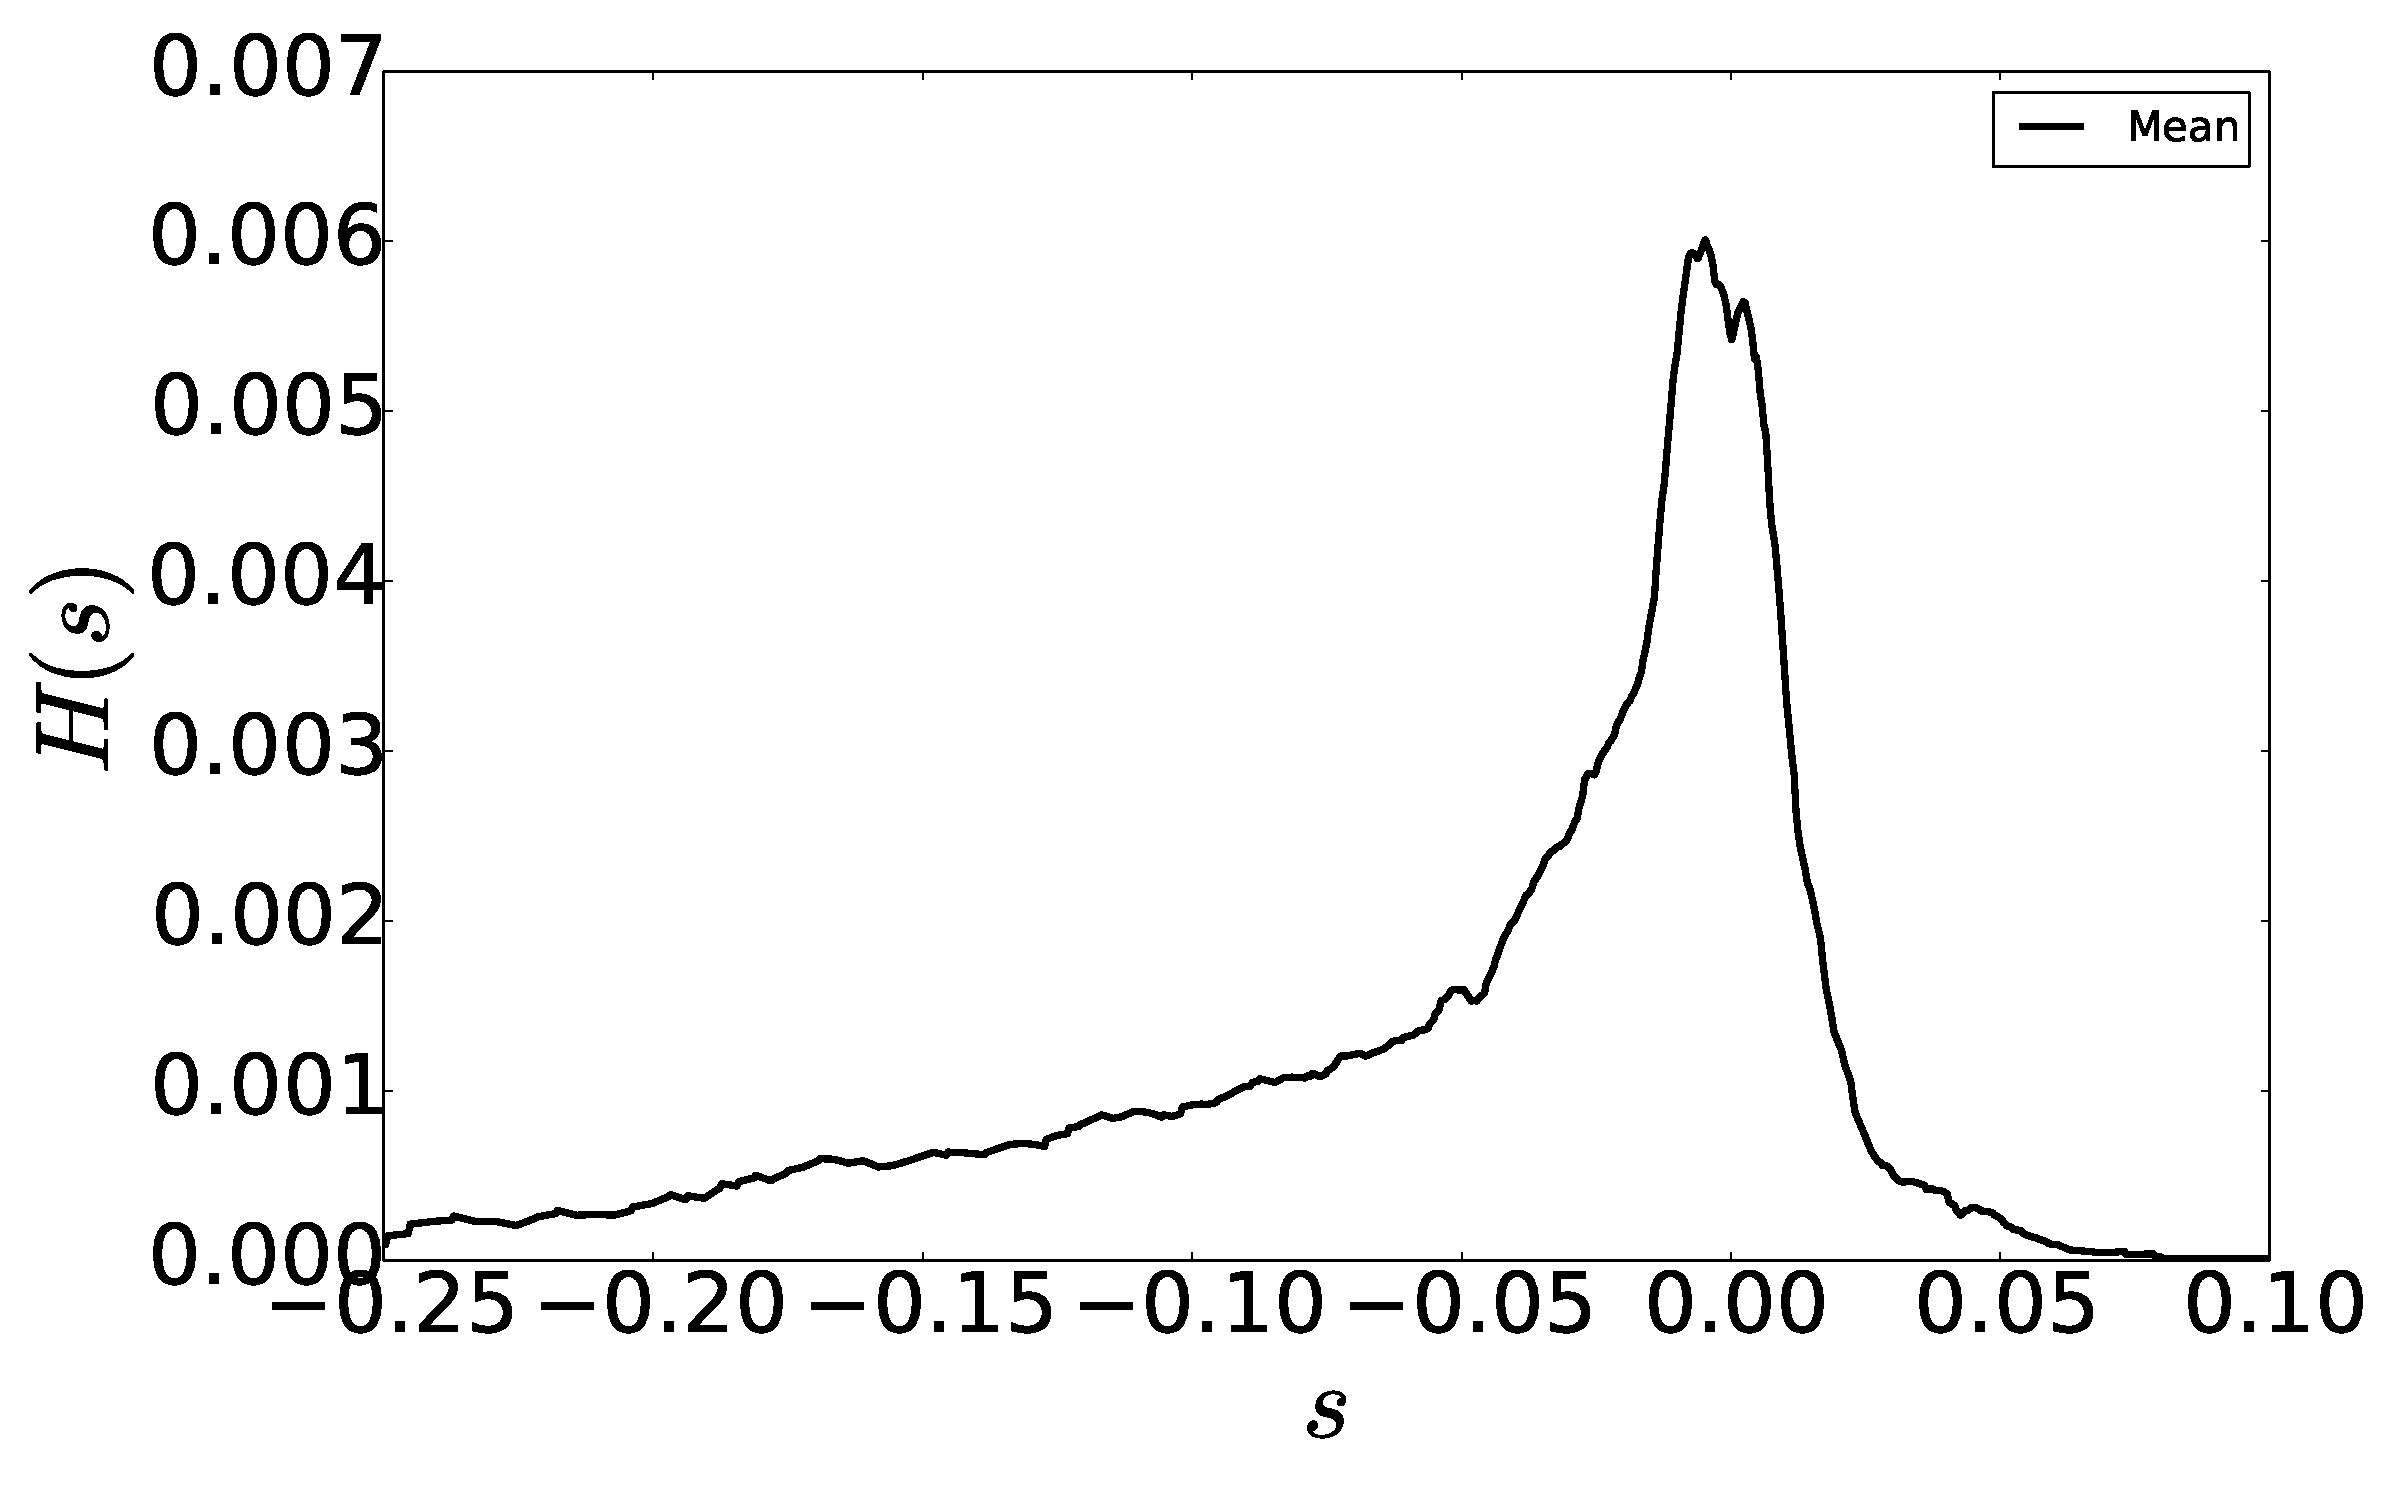
\includegraphics[width=0.35\textwidth]{MeanCluster1}}
      \subfigure[POD Modes]{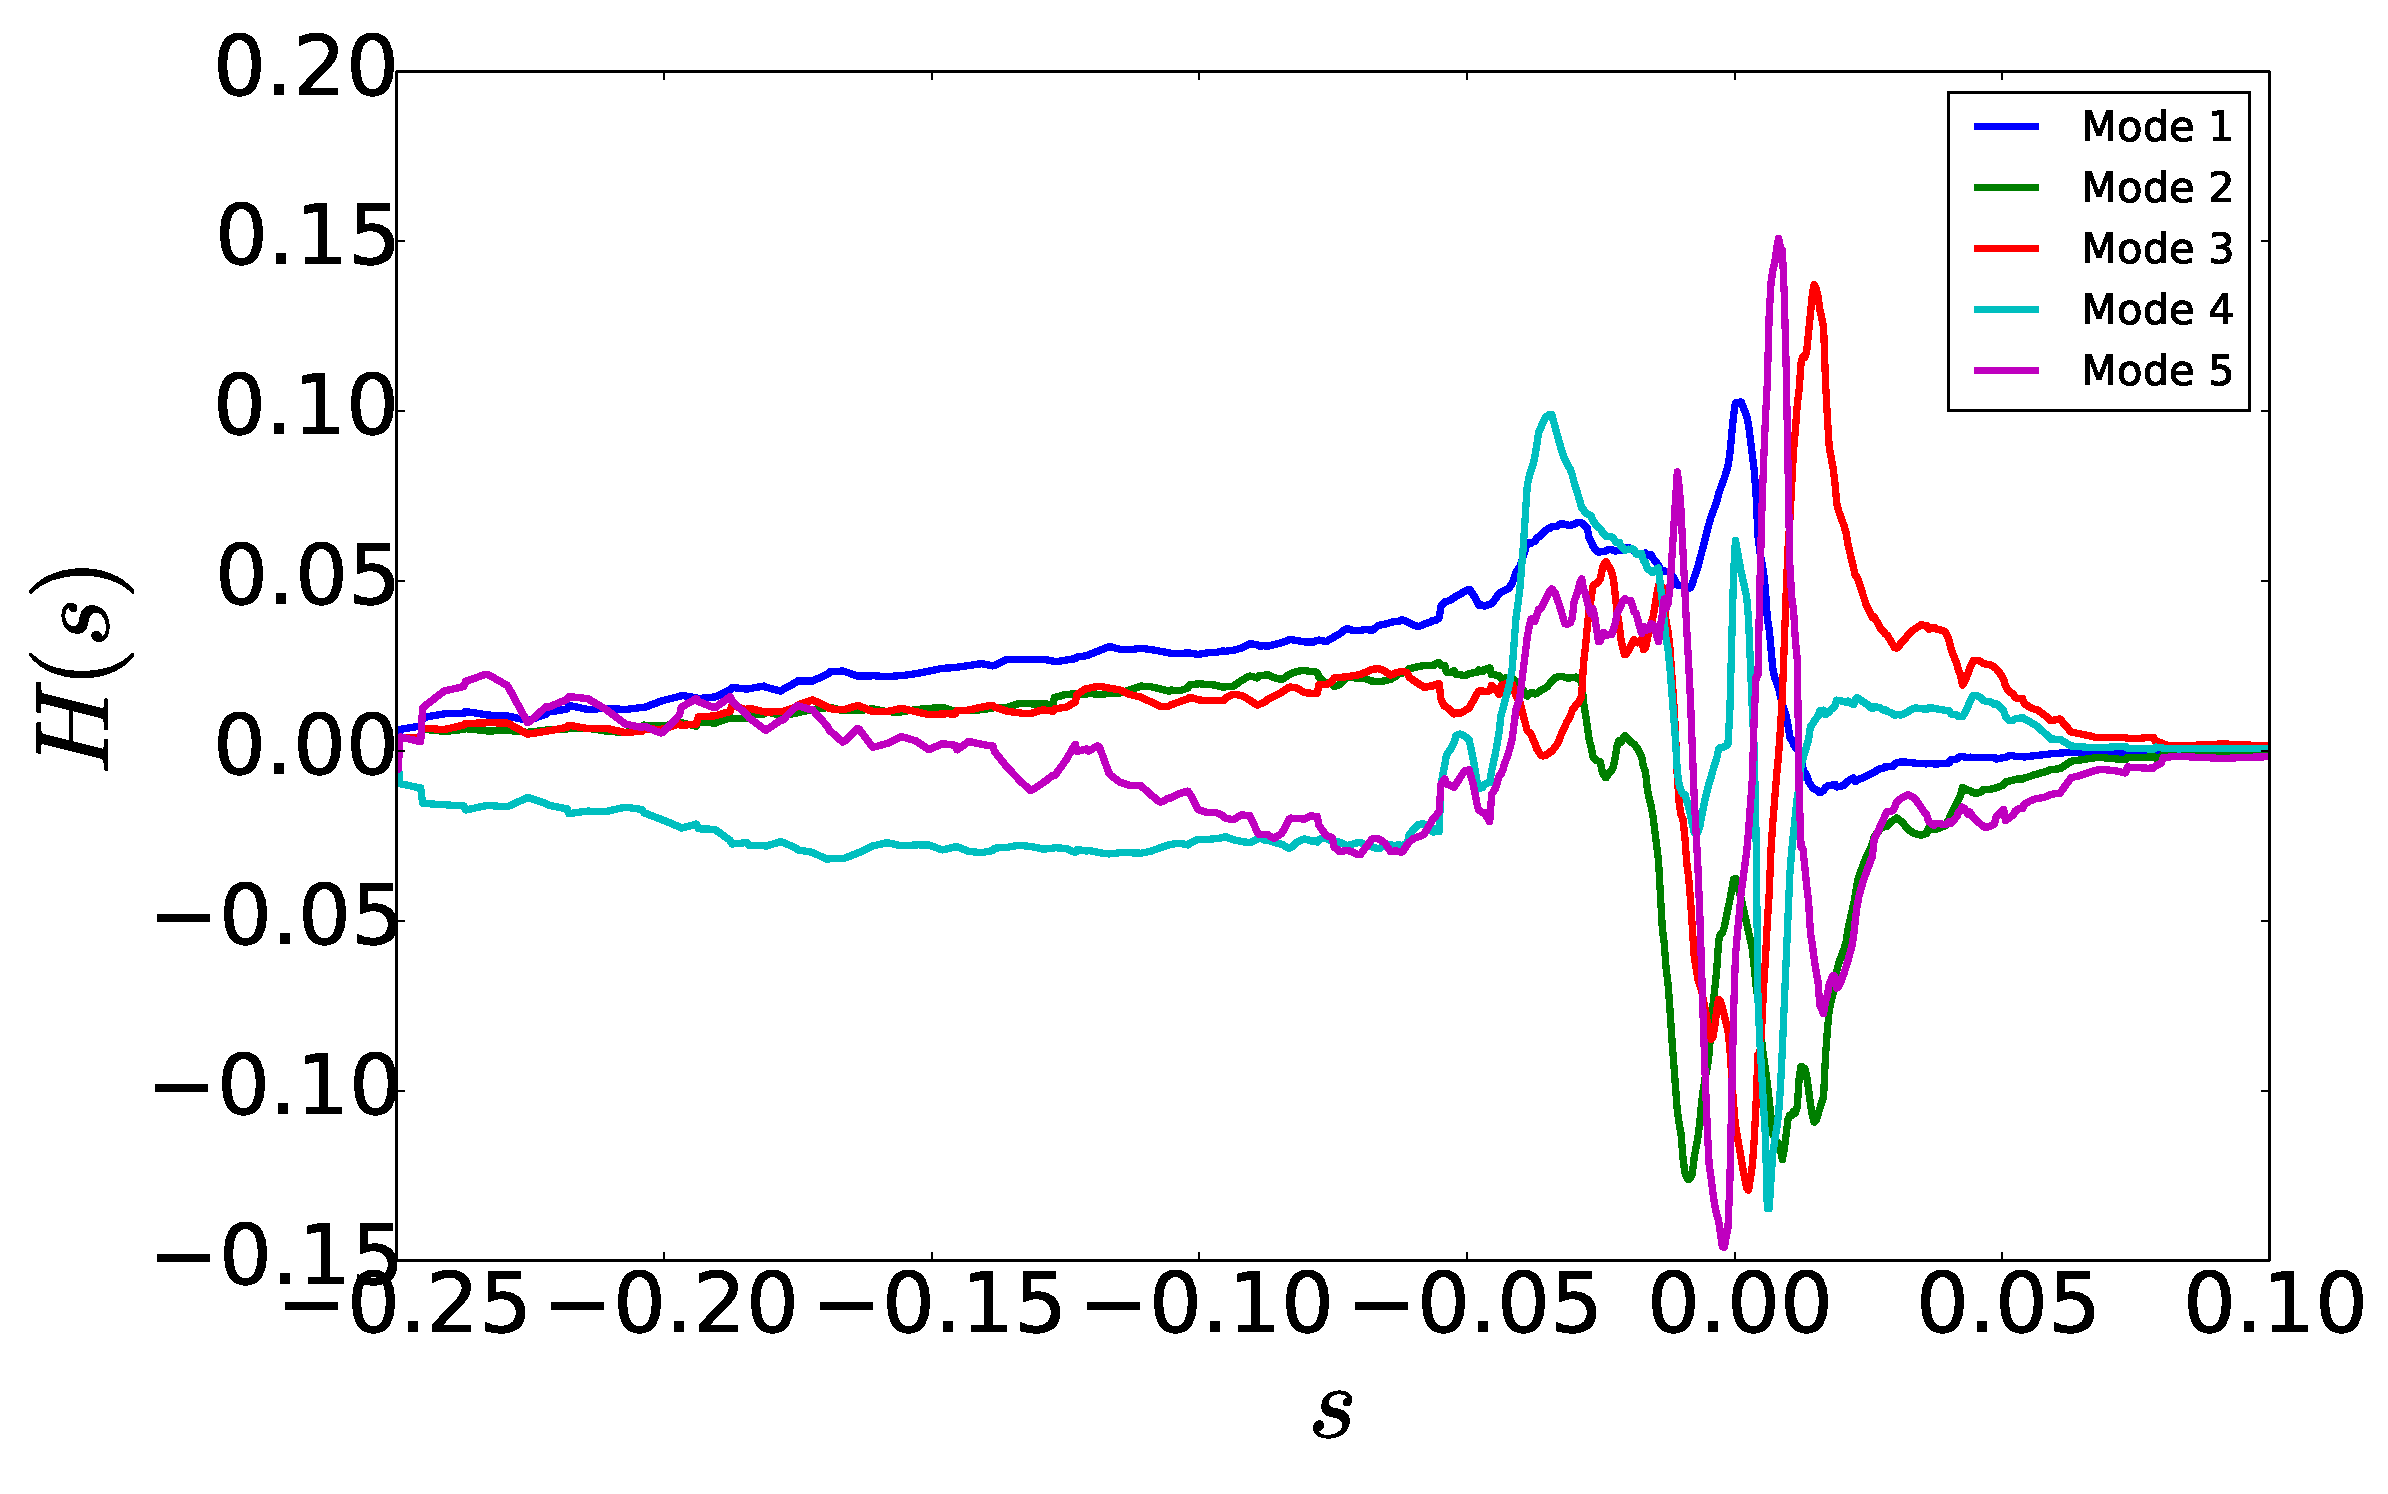
\includegraphics[width=0.35\textwidth]{PODmodes1to5Cluster1}}
      \caption{POD of ice shape cluster}
\end{figure}
\textbf{Goal:} build a low-dimensional model of ice shape cluster for UQ
\end{frame}
\begin{frame}
\frametitle{Cluster Modeling}
\label{sec-3-16}

\vspace*{-0.0cm}\begin{figure}
      \subfigure[Mode 1]{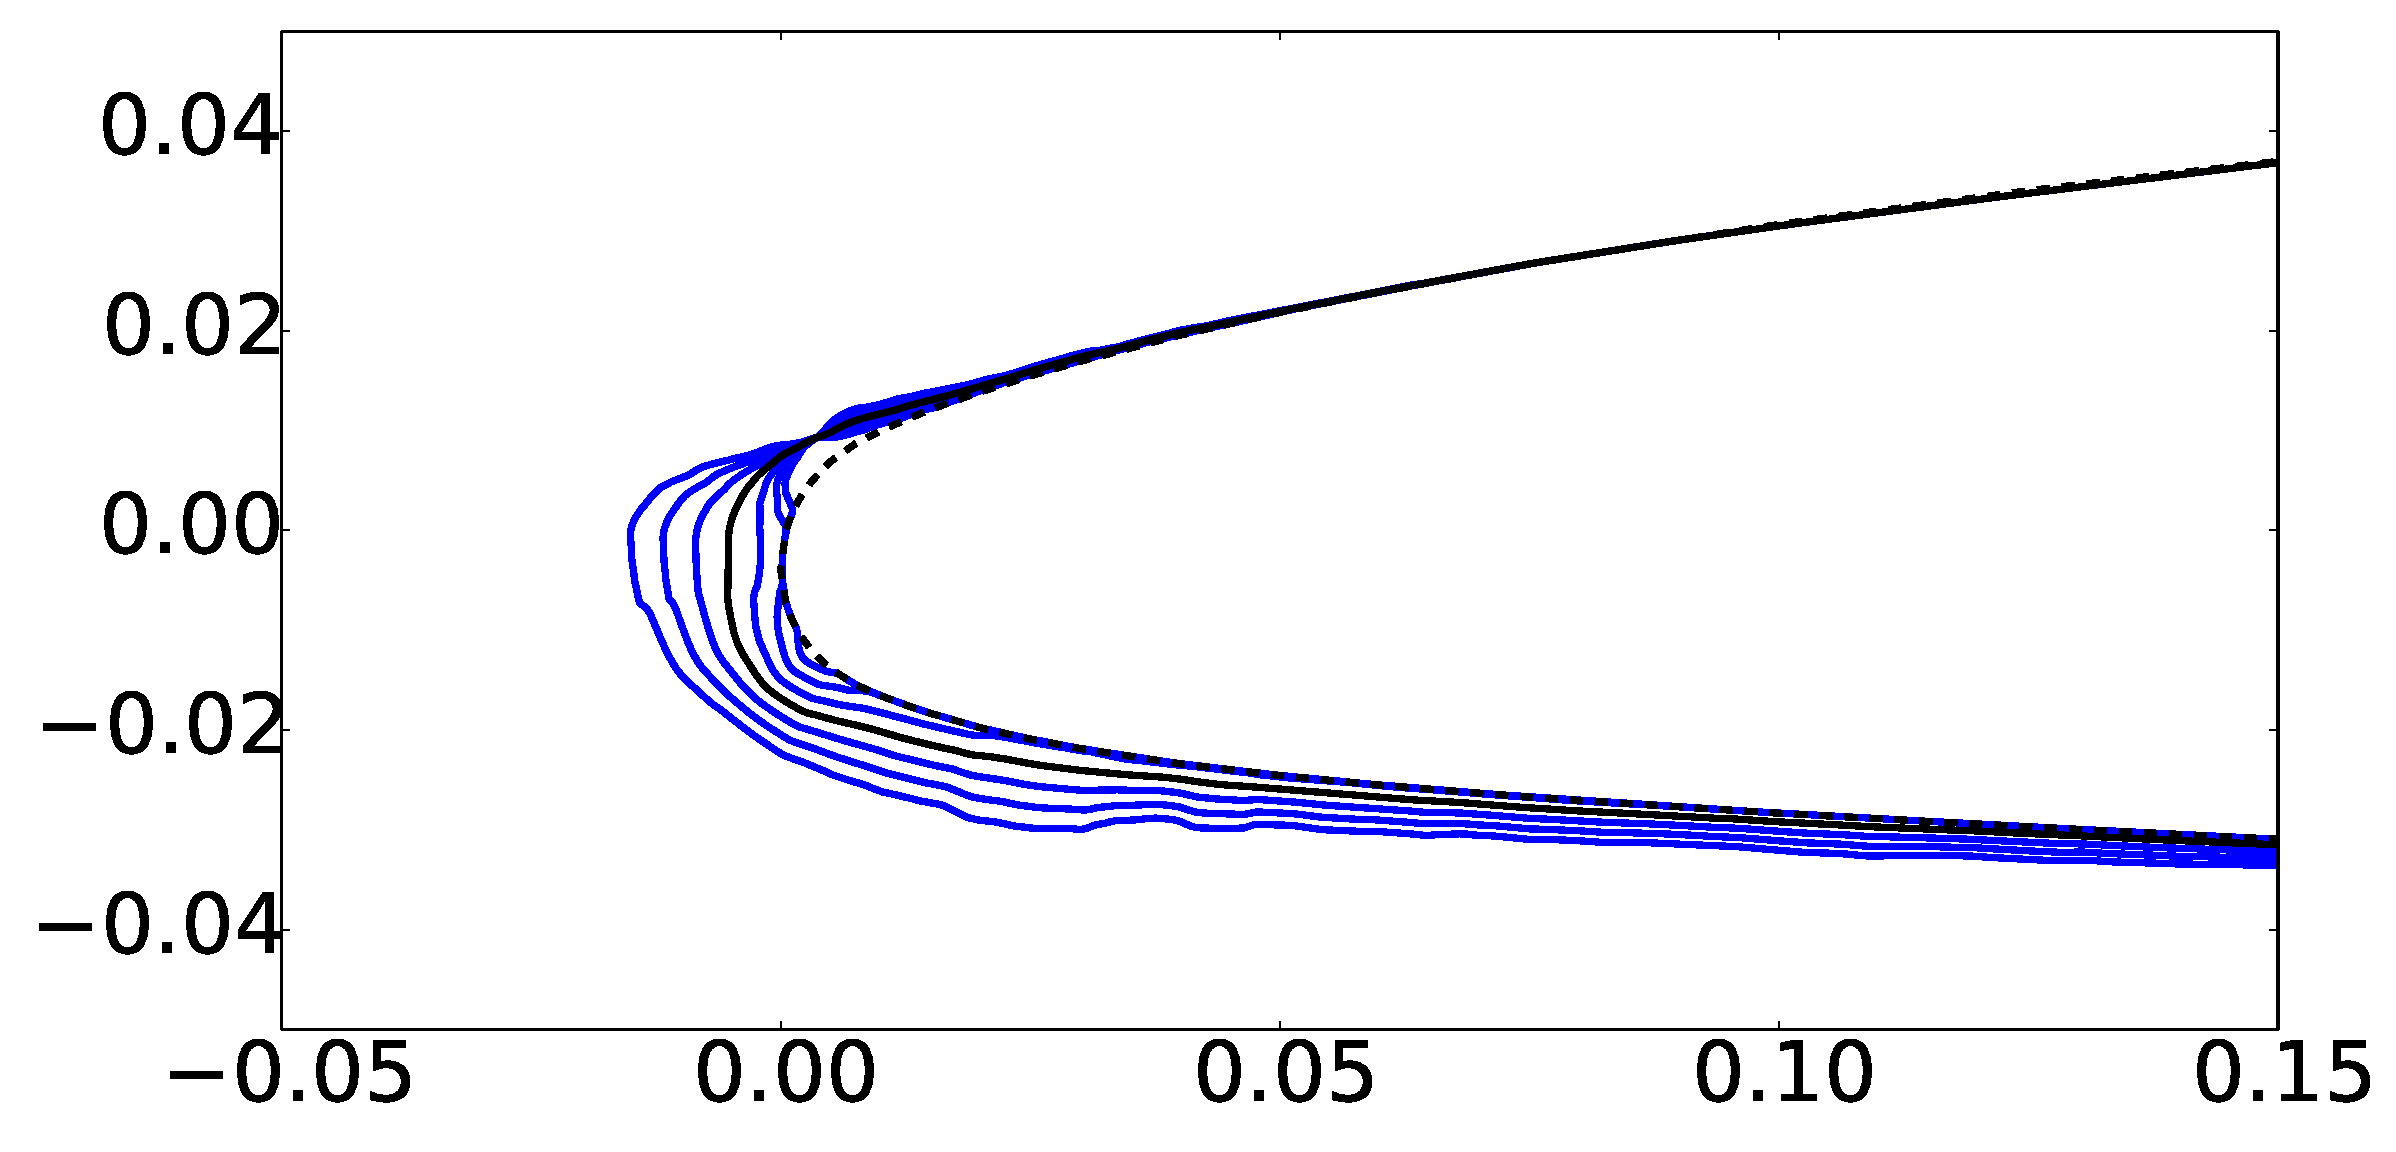
\includegraphics[width=0.3\textwidth]{POD1Shapes3Sig}}
      \subfigure[Mode 2]{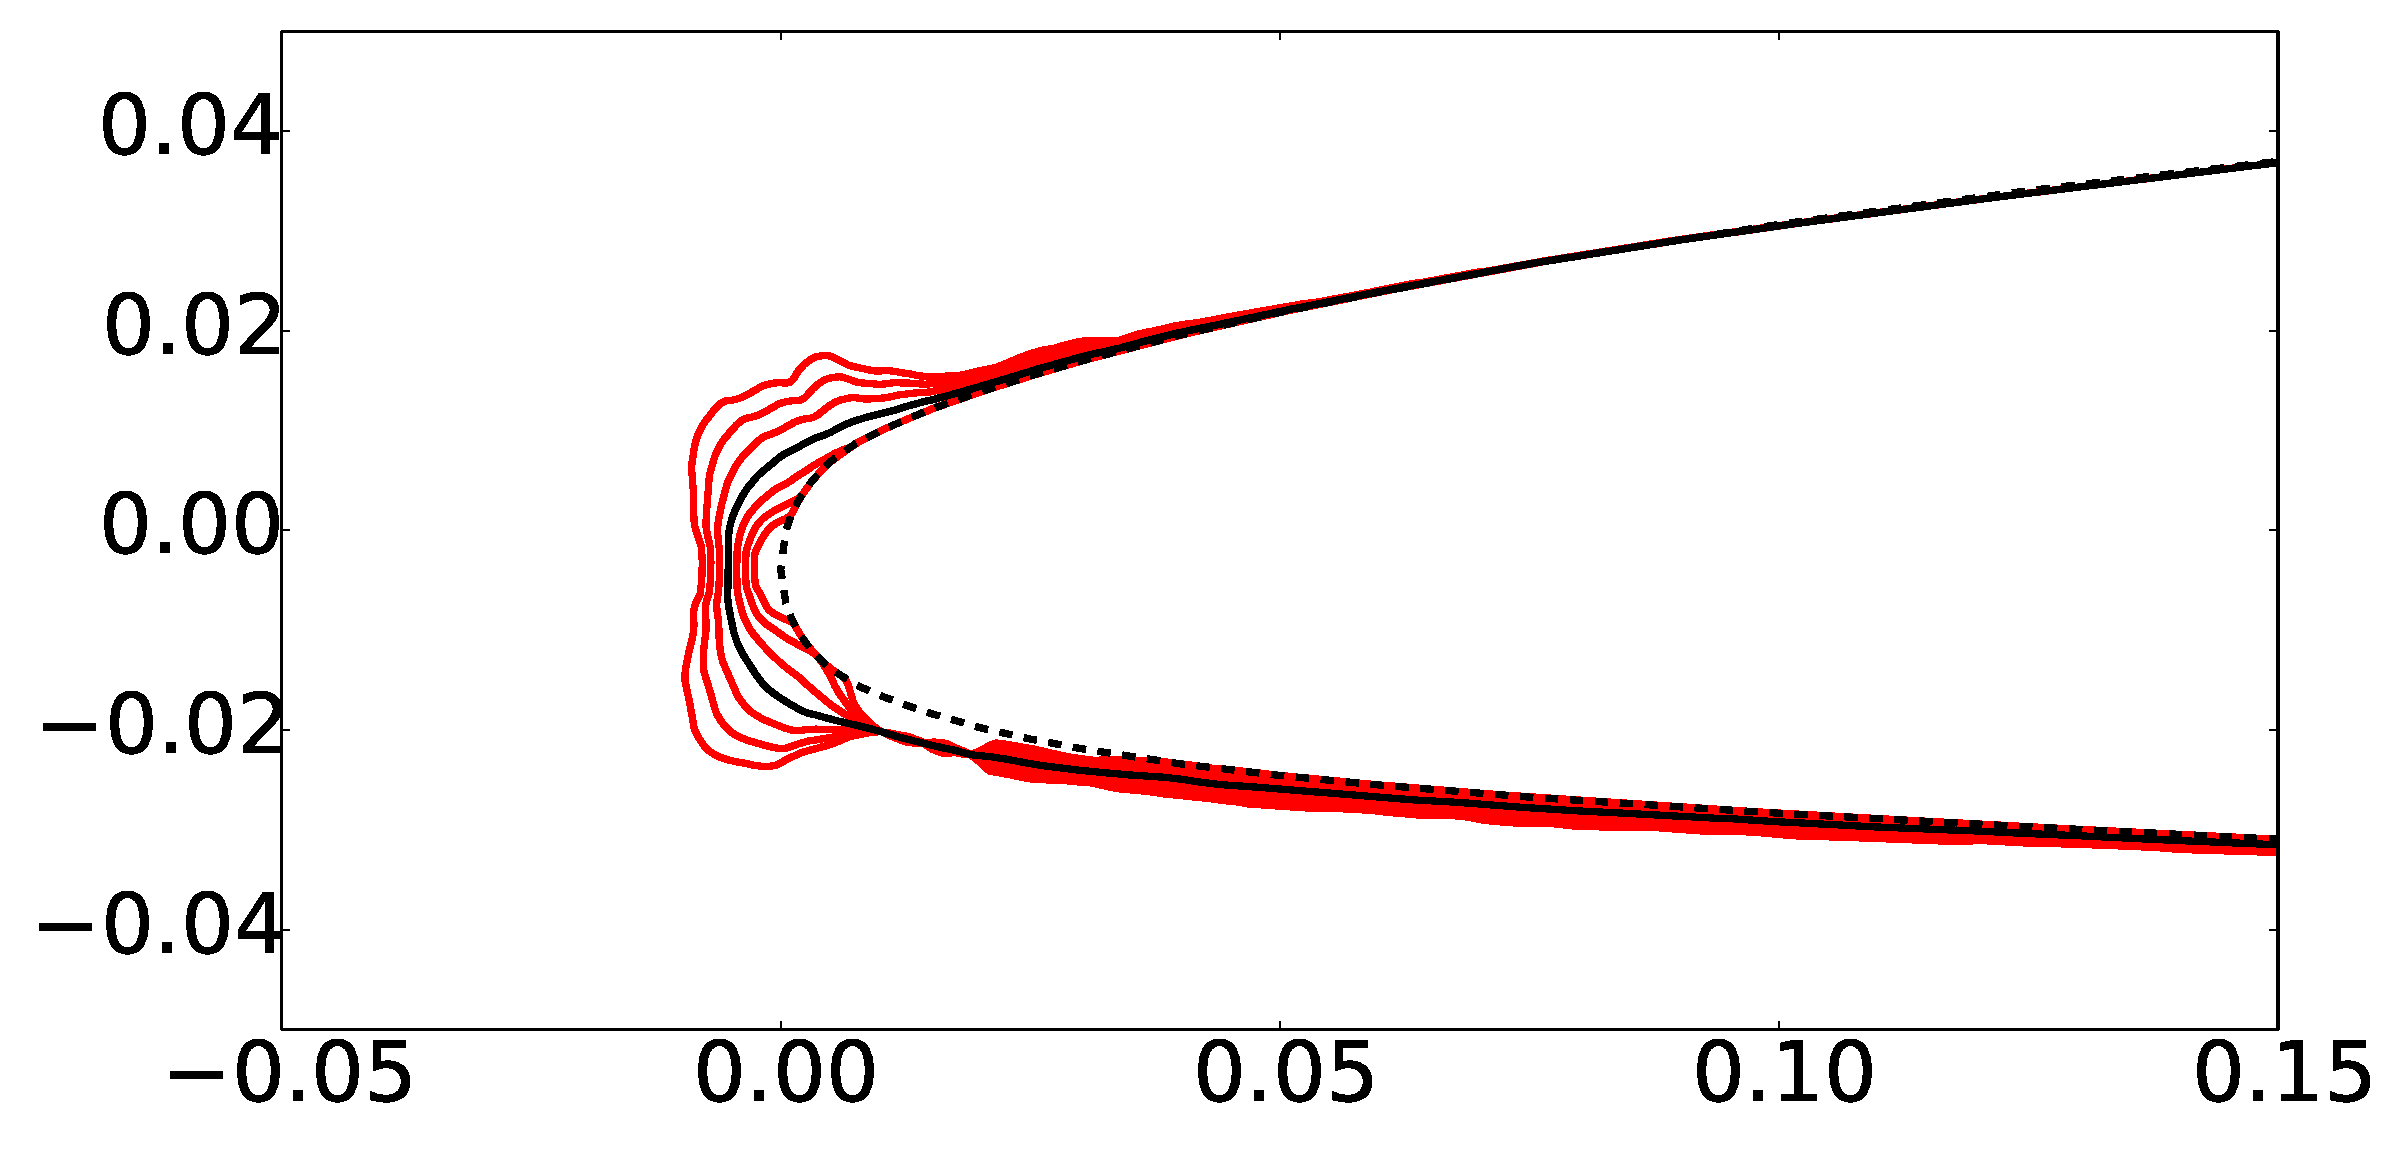
\includegraphics[width=0.3\textwidth]{POD2Shapes3Sig}}
      \subfigure[Mode 3]{\includegraphics[width=0.3\textwidth]{POD3Shapes3Sig}}
      \subfigure[Mode 4]{\includegraphics[width=0.3\textwidth]{POD4Shapes3Sig}}
      \subfigure[Mode 5]{\includegraphics[width=0.3\textwidth]{POD5Shapes3Sig}}
      \caption{Ice model modes}
\end{figure}
Variations shown about dataset mean ($\pm 3 \sigma$)
\end{frame}
\begin{frame}
\frametitle{Parameter Space}
\label{sec-3-17}

\vspace*{-0.0cm}\begin{figure}
      \subfigure[Mode 1]{\includegraphics[width=0.3\textwidth]{Cluster1Coeff1PDF}}
      \subfigure[Mode 2]{\includegraphics[width=0.3\textwidth]{Cluster1Coeff2PDF}}
      \subfigure[Mode 3]{\includegraphics[width=0.3\textwidth]{Cluster1Coeff3PDF}}
      \subfigure[Mode 4]{\includegraphics[width=0.3\textwidth]{Cluster1Coeff4PDF}}
      \subfigure[Mode 5]{\includegraphics[width=0.3\textwidth]{Cluster1Coeff5PDF}}
      \caption{Mode statistics ({\color{blue} data} and {\color{red} fit})}
\end{figure}
\begin{itemize}
\item Fit a normal distribution to dataset statistics
\item 5-dimensional UQ study with all Gaussian variables
\end{itemize}
\end{frame}
\begin{frame}
\frametitle{Output Statistics}
\label{sec-3-18}

\vspace*{-0.0cm}\begin{figure}
      \subfigure[PDF($C_L$)]{\includegraphics[width=0.4\textwidth]{PDFCLTOL1em4}}
      \subfigure[PDF($C_D$)]{\includegraphics[width=0.4\textwidth]{PDFCDTOL1em4}}
      \caption{Output PDFs for lift and drag}
\end{figure}
\begin{itemize}
\item Compute PC surrogate model using anisotropic sparse grid (487 solver
  evaluations)
\item Approximate PDFs for output metrics $C_L$ and $C_D$
\end{itemize}
\end{frame}
\begin{frame}
\frametitle{Global Extrema}
\label{sec-3-19}

\vspace*{-0.0cm}\begin{figure}
      \subfigure[Highest decile of $C_L$]{\includegraphics[width=0.3\textwidth]{BoxplotHighCL}}
      \subfigure[Lowest decile of $C_L$]{\includegraphics[width=0.3\textwidth]{BoxplotLowCL}}
      \subfigure[Means of top and bottom deciles]{\includegraphics[width=0.3\textwidth]{GoodBadAirfoils}}
      \caption{Global extrema visualized}
\end{figure}
\begin{itemize}
\item \textbf{Good:} low accretion, smooth, conforms to airfoil surface
\item \textbf{Bad:} high accretion, horns, protrude out as flow obstacles
\end{itemize}
\end{frame}
\section{Computational UQ}
\label{sec-4}
\begin{frame}
\frametitle{Motivation}
\label{sec-4-1}

\begin{itemize}
\item \textbf{Investigate uncertainty in the physical process of icing}
\begin{itemize}
\item What is the statistical effect of uncertainty in physical parameters?
\begin{itemize}
\item Free-stream temperature
\item Angle of attack
\item Convective heat transfer
\item Droplet diameter distribution
\item Accretion time
\end{itemize}
\end{itemize}
\end{itemize}
\end{frame}
\begin{frame}
\frametitle{Airfoil Icing Code Flowchart}
\label{sec-4-2}

\fontsize{7}\selectfont
% Define the layers to draw the diagram
\pgfdeclarelayer{background}
\pgfdeclarelayer{foreground}
\pgfsetlayers{background,main,foreground}

% Define block styles used later

\tikzstyle{sensor}=[draw, fill=blue!20, text width=5em, 
    text centered, minimum height=2.5em,drop shadow]
\tikzstyle{ann} = [above, text width=5em, text centered]
\tikzstyle{wa} = [sensor, text width=7.5em, fill=blue!20, 
    minimum height=3em, rounded corners, drop shadow]

% Define distances for bordering
\def\blockdist{2.3}
\def\edgedist{2.5}

\begin{tikzpicture}
    \node (CleanAirfoil) [wa]  {Clean Airfoil Geometry};
    \path (CleanAirfoil)+(4,2.5) node (FlowSolver) [wa] {Mesh/Flow Solver};
    \path (FlowSolver)+(0,-1.25) node (Droplet) [wa] {Droplet\\Advection Module};
    \path (Droplet)+(0,-1.25) node (ThermoModule) [wa] {Thermodynamic Module};
    \path (ThermoModule)+(0,-1.25) node (IcedAirfoil) [wa] {Iced Airfoil Geometry};
    \path (CleanAirfoil)+(8,0) node (FinalAirfoil) [wa] {Final Iced Airfoil Geometry};

    \path [draw, ->, thick] (CleanAirfoil.north) |- node [above] {} (FlowSolver.west);
    \path [draw, ->, thick] (FlowSolver.south) -- node [below] {} (Droplet.north);
    \path [draw, ->, thick] (Droplet.south) -- node [below] {} (ThermoModule.north);
    \path [draw, ->, thick] (ThermoModule.south) -- node [below] {} (IcedAirfoil.north);
    \path [draw, ->, thick] (IcedAirfoil.east) -| node [above] {} (FinalAirfoil.south);
    \path [draw, ->, thick] (IcedAirfoil.east) -- ++(0.75,0cm) |- node [above]
                      {} (FlowSolver.east);

    \begin{pgfonlayer}{background}
        \path (FlowSolver.west)+(-1,1) node (a) {};
        \path (IcedAirfoil.east)+(1,-1) node (b) {};
        \path[fill=orange!20,rounded corners, draw=black!50, dashed] (a) rectangle (b);
            
    \end{pgfonlayer}

\end{tikzpicture}
\end{frame}
\begin{frame}
\frametitle{Droplet Advection}
\label{sec-4-3}

\begin{equation*}
  \begin{align}
    \frac{d \bv{x}}{d t} &= \bv{v} \\
    m \frac{d \bv{v}}{d t} &= \frac{1}{2} \rho_g C_D \pi r^2 ||\bv{v_g} - \bv{v}|| (\bv{v_g} - \bv{v}) + m \bv{g}
  \end{align}
\end{equation}

\begin{columns}[c]
  \column{0.5\textwidth}
    \centering
    \includegraphics[width=1\textwidth]{ExampleR10em6} \\
    {\bf R = 10$\mu$m}
  \column{0.5\textwidth}
    \centering
    \includegraphics[width=1\textwidth]{ExampleR100em6} \\
    {\bf R = 100$\mu$m}
\end{columns}
\end{frame}
\begin{frame}
\frametitle{Thermodynamics}
\label{sec-4-4}

\begin{equation*}
  \begin{align}
    \rho_w \left \lbrace \frac{\partial h_f}{\partial t} + \nabla \cdot (\bv{u_f} h_f) \right \rbrace &= \dot{m}_{imp} - \dot{m}_{ice} \\
    \rho_w \left \lbrace \frac{\partial (h_f c_W T)}{\partial t} + \nabla \cdot (\bv{u_f} h_f c_W T) \right \rbrace &= \left [ c_W T_d + \frac{u_d^2}{2} \right ] \dot{m}_{imp} \\
    & +(L_{fus} - c_{ice}T)\dot{m}_{ice} \\
    & + c_H (T_{\infty} - T)
  \end{align}
\end{equation}

\begin{itemize}
\item \textbf{Mass}
\begin{itemize}
\item Enters through impinging droplets
\item Exits via evaporation/sublimation and freezing
\end{itemize}
\item \textbf{Energy}
\begin{itemize}
\item Enters through impinging droplets, freezing of ice
\item Exits via evaporation/sublimation, radiation, convection
\end{itemize}
\item Solved explicitly using finite volume discretization with Roe scheme upwinding
\end{itemize}
\end{frame}
\begin{frame}
\frametitle{Preliminary Intermediate Results: Ice Shapes}
\label{sec-4-5}

    \centering
    \includegraphics[width=0.65\textwidth]{Rime405Example.png}

\begin{itemize}
\item NACA0012, $\alpha = 4^o$, $T_{\infty} = 256 K$, $U_{\infty}$ = 103 m/s, MVD = 20 $\mu m$, LWC = 0.55 g/m$^3$, Re = 4.14 million, $\Delta T$ = 7 min
\item Low temperatures: convective heat transfer high enough to freeze all incoming droplets instantly (rime)
\end{itemize}
\end{frame}
\begin{frame}
\frametitle{Work In-Progress}
\label{sec-4-6}

\begin{itemize}
\item Implement rough-wall extension in Spalart-Almaras turbulence model
\item Implement neglected mass/energy transfer mechanisms
\item Verify icing calculations against published results
\item Perform UQ studies, investigate sensitivity to physical parameters
\begin{itemize}
\item Temperature, convective heat transfer coefficient, Reynolds number, MVD, LWC, angle of attack, etc.
\end{itemize}
\end{itemize}
\end{frame}

\end{document}
